% $Id: Note_ResFit_Main.tex,v 1.3 2010/07/07 09:29:40 mschrode Exp $

% =====  HEADER  ========================================

% ----- Document ----------------------------------------
\documentclass[a4paper]{cmspaper} %USE for CMS machines


% ----- User defined commands ---------------------------
% $ Id: $

% Required pacakges
\usepackage{amsmath}
\usepackage{cancel}
\usepackage{xspace}

% Sectioning
\newcommand{\qsec}[1]{Section~\ref{#1}}
\newcommand{\qfig}[1]{Fig.~\ref{#1}}
\newcommand{\qtab}[1]{Table~\ref{#1}}
\newcommand{\qeq}[1]{\eqref{#1}}

% Units
\newcommand{\tev}{\ensuremath{\;\text{Te}\kern-0.06667em\text{V}}\xspace}
\newcommand{\gev}{\ensuremath{\;\text{Ge}\kern-0.06667em\text{V}}\xspace}
\newcommand{\mev}{\ensuremath{\;\text{Me}\kern-0.06667em\text{V}}\xspace}
\newcommand{\km}{\ensuremath{\;\text{km}}\xspace}
\newcommand{\m}{\ensuremath{\;\text{m}}\xspace}
\newcommand{\cm}{\ensuremath{\;\text{cm}}\xspace}
\newcommand{\mm}{\ensuremath{\;\text{mm}}\xspace}
\newcommand{\second}{\ensuremath{\;\text{s}}\xspace}
\newcommand{\tons}{\ensuremath{\;\text{t}}\xspace}
\newcommand{\tesla}{\ensuremath{\;\text{T}}\xspace}
\newcommand{\kelvin}{\ensuremath{\;\text{K}}\xspace}
\newcommand{\pbinv}{\ensuremath{\;\text{pb}^{-1}}\xspace}

% Quantities
\newcommand{\et}{\ensuremath{E_{\text{T}}}\xspace}
\newcommand{\met}{\ensuremath{\slash\mkern-12mu{E}_{\text{T}}}\xspace}
\newcommand{\mht}{\ensuremath{\slash\mkern-12mu{H}_{\text{T}}}\xspace}
\newcommand{\metvec}{\ensuremath{\slash\mkern-12mu{\vec{E}}_{\text{T}}}\xspace}
\newcommand{\pt}{\ensuremath{p_{\text{T}}}\xspace}
\newcommand{\pti}[1]{\ensuremath{p_{\text{T},#1}}\xspace}
\newcommand{\ptvec}{\ensuremath{\vec{p}_{\text{T}}}\xspace}
\newcommand{\ptsub}[1]{\ensuremath{p_{\text{T},#1}}\xspace}
\newcommand{\ptvecsub}[1]{\ensuremath{\vec{p}_{\text{T},#1}}\xspace}
\newcommand{\ptdijet}{\ensuremath{p^{\text{dijet}}_{\text{T}}}\xspace}
\newcommand{\ptgen}{\ensuremath{p^{\text{gen}}_{\text{T}}}\xspace}
\newcommand{\pthat}{\ensuremath{\hat{p}_{\text{T}}}\xspace}
\newcommand{\pttrue}{\ensuremath{p^{\text{true}}_{\text{T}}}\xspace}
\newcommand{\pttruehigh}[1]{\ensuremath{p^{\text{true,#1}}_{\text{T}}}\xspace}
\newcommand{\ptrel}{\ensuremath{p^{\text{rel}}_{\text{T},3}}\xspace}
\newcommand{\ptmeas}{\ensuremath{p^{\text{meas}}_{\text{T}}}\xspace}
\newcommand{\ptmeasi}[1]{\ensuremath{p^{\text{meas}}_{\text{T},#1}}\xspace}
\newcommand{\ptcalo}{\ensuremath{p^{\text{calo}}_{\text{T}}}\xspace}
\newcommand{\ptcaloi}[1]{\ensuremath{p^{\text{calo}}_{\text{T},#1}}\xspace}
\newcommand{\ptmin}{\ensuremath{\pt^{\text{min}}}\xspace}
\newcommand{\ptmax}{\ensuremath{\pt^{\text{max}}}\xspace}
\newcommand{\ptparticle}{\ensuremath{\pt(\text{particle})}\xspace}
\newcommand{\ptreco}{\ensuremath{\pt(\text{reco})}\xspace}

% Symbols
\newcommand{\dif}[1]{\ensuremath{\text{d}#1}\xspace}
\newcommand{\e}{\,\text{e}}
\newcommand{\nup}[1]{$^{\text{\scriptsize #1}}$}
\newcommand{\dgr}{\ensuremath{\,^{\circ}}}
\newcommand{\mean}[1]{\ensuremath{\langle#1\rangle}}
\newcommand{\gqq}[1]{\ensuremath{\glqq#1\grqq}}
\newcommand{\rarr}{\ensuremath{\rightarrow}\xspace}

% Words and characters
\newcommand{\diagonalsout}[1]{\ensuremath{\cancel{\text{#1}}}}
\newcommand{\genjet}{GenJet\xspace}
\newcommand{\genjets}{GenJets\xspace}
\newcommand{\calojet}{CaloJet\xspace}
\newcommand{\calojets}{CaloJets\xspace}




% ----- Additional packages -----------------------------
\usepackage{subfigure}
\usepackage{booktabs}


% ----- pdflatex setup ----------------------------------
\usepackage[pdftex]{color,graphicx}
\usepackage[pdftex]{hyperref}
\hypersetup{unicode=true}
\hypersetup{bookmarks=true}
\hypersetup{pdftitle={Determination of the Jet Energy Resolution in QCD Dijet Events}}
\hypersetup{pdfauthor={Matthias Schr\"oder}}
\hypersetup{colorlinks=true}



% =====  DOCUMENT  ======================================

\begin{document}


% ----- Title page and TOC ------------------------------
\begin{titlepage}
  \date{\today}
  \title{Determination of the Jet Energy Resolution in QCD Dijet
    Events using an Unbinned Maximum Likelihood Method}
\end{titlepage}
\tableofcontents


% ----- Main part from external files -------------------
% $Id: Note_ResFit_Introduction.tex,v 1.4 2010/06/01 17:24:50 mschrode Exp $


\section{Introduction}

The analysis of jet final states provides an important way to investigate Standard Model and beyond processes and requires a precise knowledge of the jet transverse momentum, \textit{\pt}, resolution.

In this note the jet response, \textit{R}, is defined as the ratio of the measured detector level jet \pt and the underlying particle level jet \pt, \textit{\ptparticle}.
The jet response distribution for a constant \ptparticle follows a Gaussian in good approximation.
Therefore the jet resolution is defined as the standard deviation of the jet response distribution at a given \ptparticle.

\textit{
\begin{itemize}
\item Gaussian core: calorimeter measurement
\item Low tail: punch-through; $\mu$, $\nu$ from heavy flavour jets
\item High tail: non-linearities of calorimeter
\end{itemize}
}

In this note a method is presented to derive the jet transverse momentum, \pt, resolution from QCD dijet events in collider data.
Dijet events have a large cross section e.g. in comparison to $\gamma$-jet events and hence provide a higher \pt reach and an early sensitivity also to non-Gaussian tails of the jet response function.

A likelihood function is constructed with probability densities, \textit{pdf}s, of the \pt imbalance in the dijet event.
The pdfs are a convolution of the particle level jet differential cross section with suitable parameterisations of the jet \pt response functions.
As a consequence, the measured resolution is parametrised as a function of particle level jet \pt.
In addition, a description of selection biases arising from requirements on the measured jet \pt is incorporated.

The method is strictly valid in the ideal case of events with only two jets in the final state, that are balanced in \pt at the particle level, and under the assumption that detector response and resolution effects on both jets are not correlated with each other.
In real QCD events, however, the \pt balance of the two jets is affected by the presence of additional jet activity from e.g. gluon radiation and the measurement has to be corrected for this effect.

In case that other event types are included into the likelihood, such as $\gamma+$jets, suitable probability density functions must be defined.

The studies included in this note are performed on jets that have been reconstructed from calorimeter towers, \textit{\calojets}, although the method is general and may be applied to any type of detector level jet.


% $Id: Note_ResFit_Technique.tex,v 1.3 2010/05/31 13:10:51 mschrode Exp $


\section{Description of the Method}\label{sec:ResFit:Method}

\subsection{Definition of the dijet likelihood}\label{sec:ResFit:Method:Likelihood}

The underlying assumptions of the presented method are
\begin{itemize}
\item an ideal dijet event configuration with exactly two jets that
  are balanced in true transverse momentum, \mbox{$\pttrue\equiv\ptparticle$};
\item measured jet transverse momenta,
  \mbox{$\ptmeasi{i}\equiv\ptcaloi{i}$}, $i\in[1,2]$, result from uncorrelated
  calorimeter measurements.
\end{itemize}
Based on these, the pdf of a measured dijet event configuration is defined as
\begin{equation}
  \label{eq:resFit:DijetPdf}
  g_{\mathbf{\xi}}\left(\ptmeasi{1},\ptmeasi{2}\right) \propto \int^{\infty}_{0}\dif{\pttrue}\,f\left(\pttrue\right)
  \cdot r_{\mathbf{\xi}}\left(\ptmeasi{1}|\pttrue\right)
  \cdot r_{\mathbf{\xi}}\left(\ptmeasi{2}|\pttrue\right).
\end{equation}
Here,
\begin{itemize}
\item $f(\pttrue)$ denotes the pdf of the true jet \pt
  i.e. the particle level differential dijet cross section.
  In the following it is assumed to be known
  and taken from the Monte Carlo simulation
  (comp. e.g. Fig.~\ref{fig:resFit:qcd:dijetspectrum:subA}).
  Uncertainties on the simulated cross section have to be propagated to
  the measured resolution and added as a systematic uncertainty of the
  method, which is in fact small as shown in Section~\ref{};
\item $r_{\mathbf{\xi}}(\ptmeasi{i}|\pttrue)$ denotes the pdf of the measured \pt
  of the $i$-th jet.
  It is parametrised with a suitable function depending on the set of
  parameters $\mathbf{\xi}$, e.g. a Gauss or Crystal Ball function.
\end{itemize}
It is important to note that
$g_{\mathbf{\xi}}(\ptmeasi{1},\ptmeasi{2})$ does not depend on \pttrue
as this is the integration variable.

If $f(\pttrue)$ and $r_{\mathbf{\xi}}(\ptmeasi{i}|\pttrue)$ are properly normalised in the considered interval \mbox{$\pttruehigh{min} < \pttrue < \pttruehigh{max}$} such that
\begin{eqnarray*}
  1 & = & \int^{\pttruehigh{max}}_{\pttruehigh{max}}\dif{\pttrue}\,f\left(\pttrue\right) \\
  1 & = & \int^{\infty}_{0}\dif{\ptmeasi{i}}\,r_{\mathbf{\xi}}\left(\ptmeasi{i}|\pttrue\right)
\end{eqnarray*}
then also the dijet pdf is properly normalised to
\begin{equation*}
  1 = \int^{\infty}_{0}\dif{\ptmeasi{1}}\,\int^{\infty}_{0}\dif{\ptmeasi{2}}\, g_{\mathbf{\xi}}\left(\ptmeasi{1},\ptmeasi{2}\right),
\end{equation*}
provided the integration order of $\ptmeasi{i}$ and $\pttrue$ can be interchanged.

For a sample of $N$ dijet events, a likelihood is defined as
\begin{equation}
  \label{eq:ResFit:Likelihood}
  \mathcal{L}\left(\mathbf{\xi}\right) = \prod^{N}_{k=1} g_{\mathbf{\xi},k}\left(\ptmeasi{1},\ptmeasi{2}\right).
\end{equation}
Maximisation of $\mathcal{L}(\mathbf{\xi})$ then results in an
estimate of the optimal values of $\mathbf{\xi}$ for the chosen
function $r_{\mathbf{\xi}}(\ptmeasi{i}|\pttrue)$.
Note that $r_{\mathbf{\xi}}(\ptmeasi{i}|\pttrue)$ is defined as the
pdf of the measured jet \pt.
The pdf of the jet \pt response \mbox{$R_{i}\equiv\ptmeasi{i} / \pttrue$} is obtained by parameter transformation
\begin{equation*}
  r_{\mathbf{\xi}}\left(R_{i}|\pttrue\right) =
  r_{\mathbf{\xi}}\left(\ptmeasi{i}\left(R_{i}\right)|\pttrue\right)\cdot\left|\frac{\dif{\ptmeasi{i}}}{\dif{R_{i}}}\right|.
\end{equation*}



\subsection{Description of selection biases in a data driven event selection}\label{sec:ResFit:Method:Biases}

\textit{To be copied from RA2 note}

% $Id: Note_ResFit_ToyMC.tex,v 1.1 2010/05/30 19:43:08 mschrode Exp $


\section{Study with a Toy Monte Carlo Simulation}\label{sec:ResFit:ToyMC}

The method presented in the previous Section~\ref{sec:ResFit:Method}
is studied using a simple simulation, \textit{Toy Monte Carlo}.
First, the basic likelihood fit described in
Section~\ref{sec:ResFit:Method:Likelihood} is performed (Section~\ref{sec:ResFit:ToyMC:PtGenCuts}),
whereby events have been selected using Monte Carlo truth information.
Second, a data driven event selection has been applied and the
modified likelihood, described in
Section~\ref{sec:ResFit:Method:Biases}, is maximised (Section~\ref{sec:ResFit:ToyMC:PtCaloCuts}).


\subsection{Generated sample}\label{sec:ResFit:ToyMC:Sample}

A sample of $30\,000$ ideal dijet events has been generated assuming a
s imple exponential particle level jet \pt spectrum
\begin{equation}
  \label{eq:ResFit:ToyMC:Spectrum}
  f\left(\pttrue\right) \propto \exp\left(-\pttrue / \tau\right),
  \qquad \tau = 80.
\end{equation}
ranging from \mbox{$50 < \pttrue < 1000\gev$} (comp. Fig.~\ref{fig:ResFit:ToyMC:Sample:Spectrum}).
Two independent measurements of the jet \pt have been simulated by
weighting \pttrue with random numbers drawn from a Gaussian response
\begin{equation}
  \label{eq:ResFit:ToyMC:Response}
  r_{\mathbf{\xi}}\left(\ptmeas|\pttrue\right) = 
  \frac{1}{\sqrt{2\pi}\sigma}\exp\left[-\frac{1}{2}\left(\frac{\ptmeas - \pttrue}{\sigma}\right)^{2}\right]
\end{equation}
(Here and in the following the jet index $i$ has been omitted.)
The standard deviation, i.e. the jet resolution, $\sigma$ has been parameterised as a function of \pttrue and
the parameters $\xi_{i}$, \mbox{$i\in [0,2]$}, as
\begin{equation}
  \label{eq:ResFit:ToyMC:Sigma}
  \sigma = \xi_{0}\gev
  \oplus \xi_{1}\,\sqrt{\pt\gev}\oplus \xi_{2}\pt.
\end{equation}
The values of the parameters $\mathbf{\xi}$ are listed in
Tab.~\ref{tab:ResFit:ToyMC:PtGenCuts:FitResult}.
An example of a simulated response distribution is shown in Fig. ~\ref{fig:ResFit:ToyMC:PtGenCuts:Response}.

\begin{figure}[ht]
  \begin{center}
     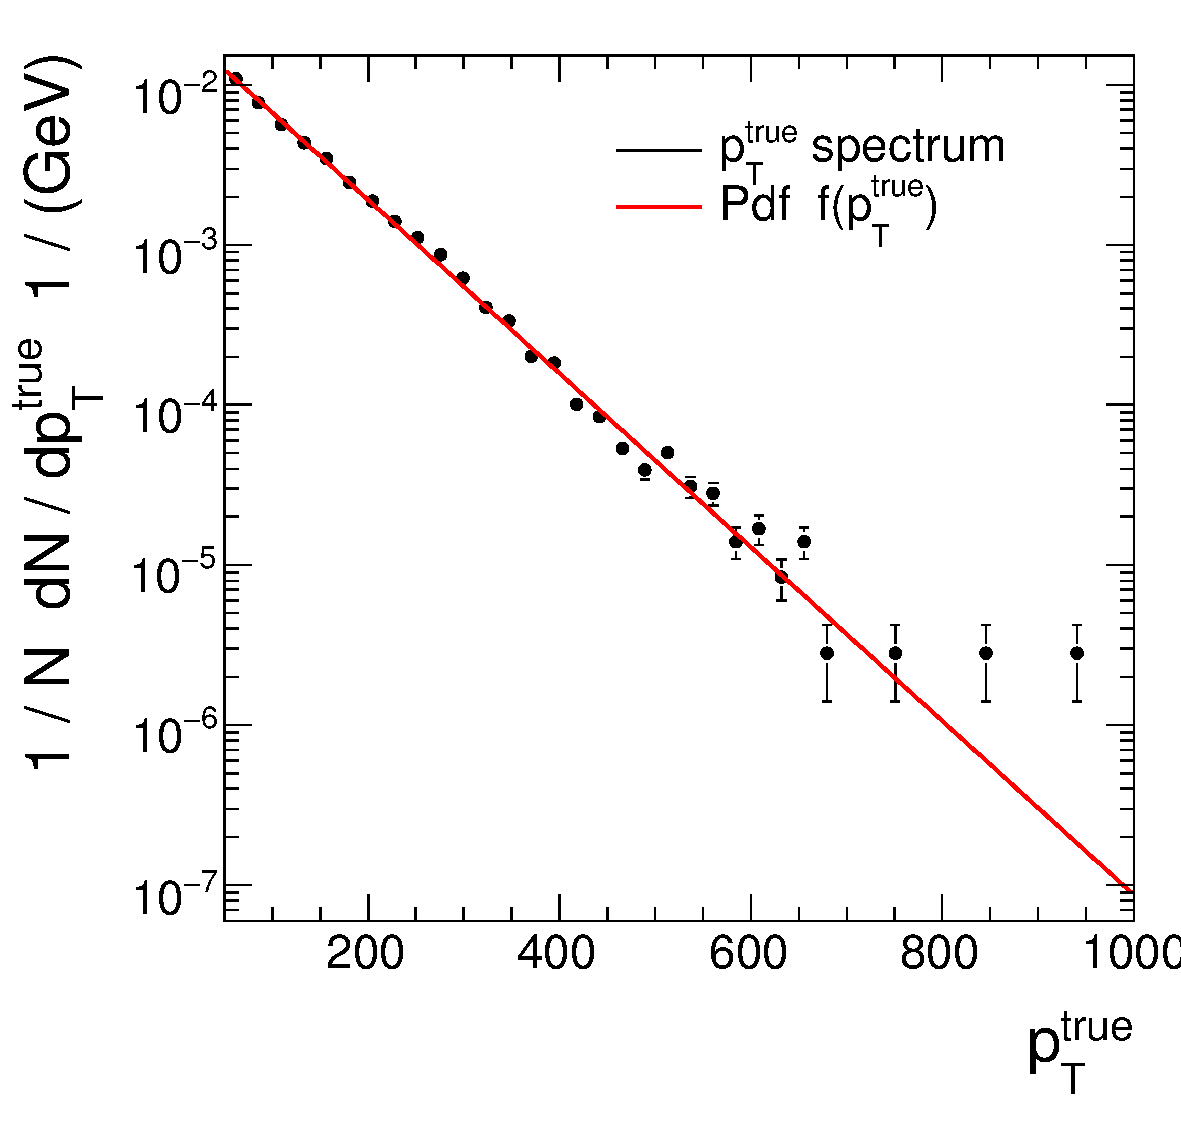
\includegraphics[width=0.45\textwidth]{figures/resFit_ToyMC_PtGenCuts_SpectrumLog}
   \end{center}
   \caption{Toy Monte Carlo simulation of a sample of ideal dijet events.
     Generated \pttrue spectrum (circular markers) and the underlying pdf (solid line).}
   \label{fig:ResFit:ToyMC:Sample:Spectrum}
\end{figure}


\subsection{Measurement of the resolution with a truth information based event selection}\label{sec:ResFit:ToyMC:PtGenCuts}

The jet energy resolution of the dijet sample is to be measured as described in Section~\ref{sec:ResFit:Method:Likelihood}.
Dijet events are have been selected from the sample described above by
requiring \mbox{$\ptmin < \pttrue < \ptmax$}.
The jet \pt spectrum is taken directly from the
simulation~\eqref{eq:ResFit:ToyMC:Spectrum}, while the jet \pt
response is assumed to be Gaussian and the resolution $\sigma$ to
depend on \pttrue and the parameters $\mathbf{\xi}$ as
in~\eqref{eq:ResFit:ToyMC:Sigma}.

\begin{figure}[ht]
  \begin{center}
    \begin{tabular}{cc}
      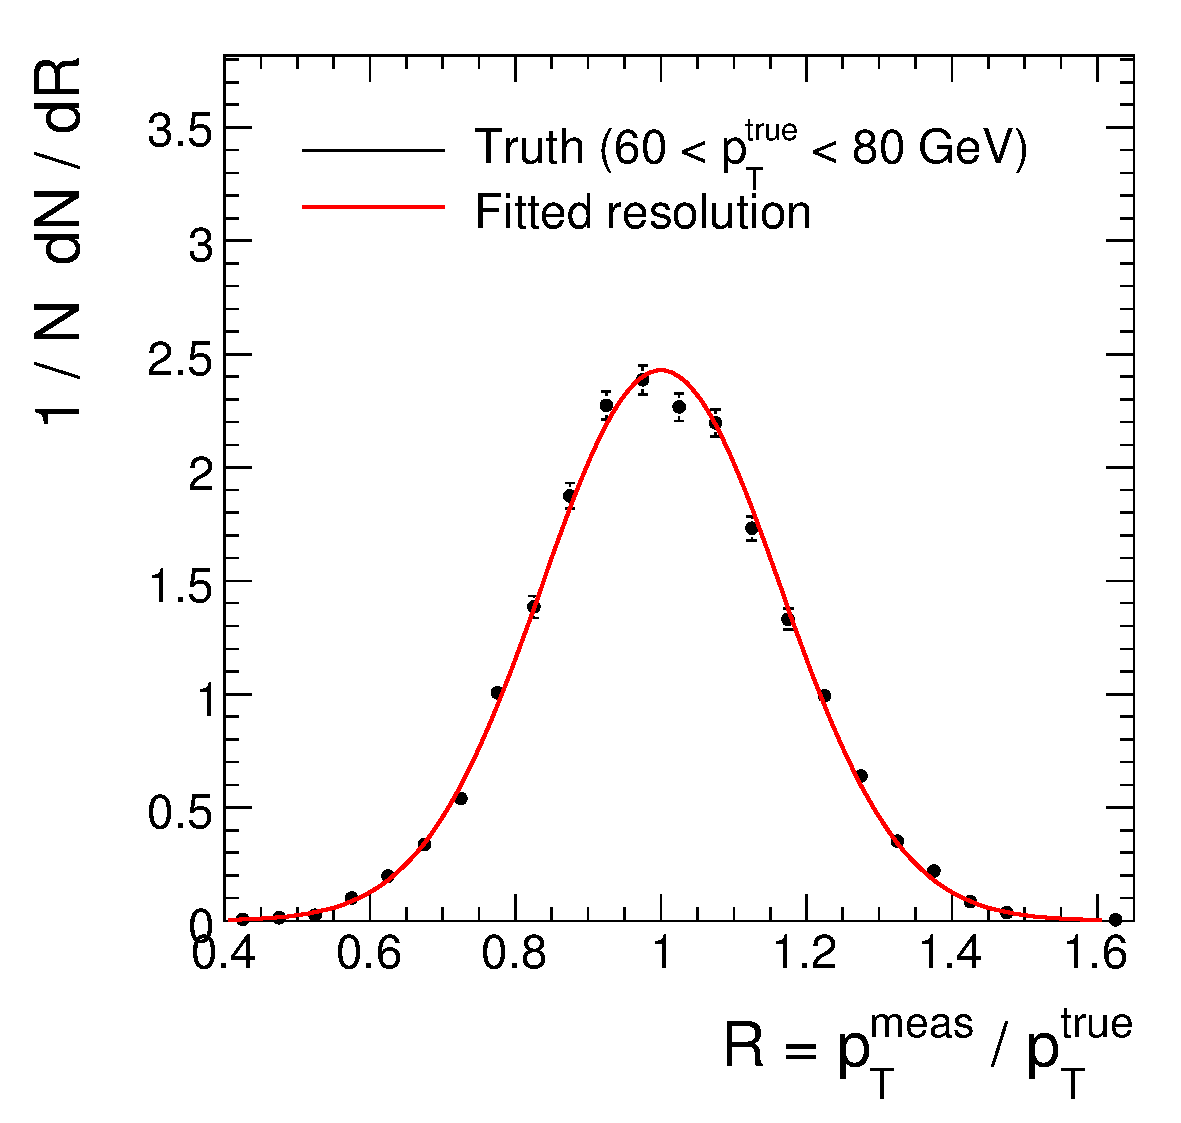
\includegraphics[width=0.45\textwidth]{figures/resFit_ToyMC_PtGenCuts_ResolutionBin1} &
      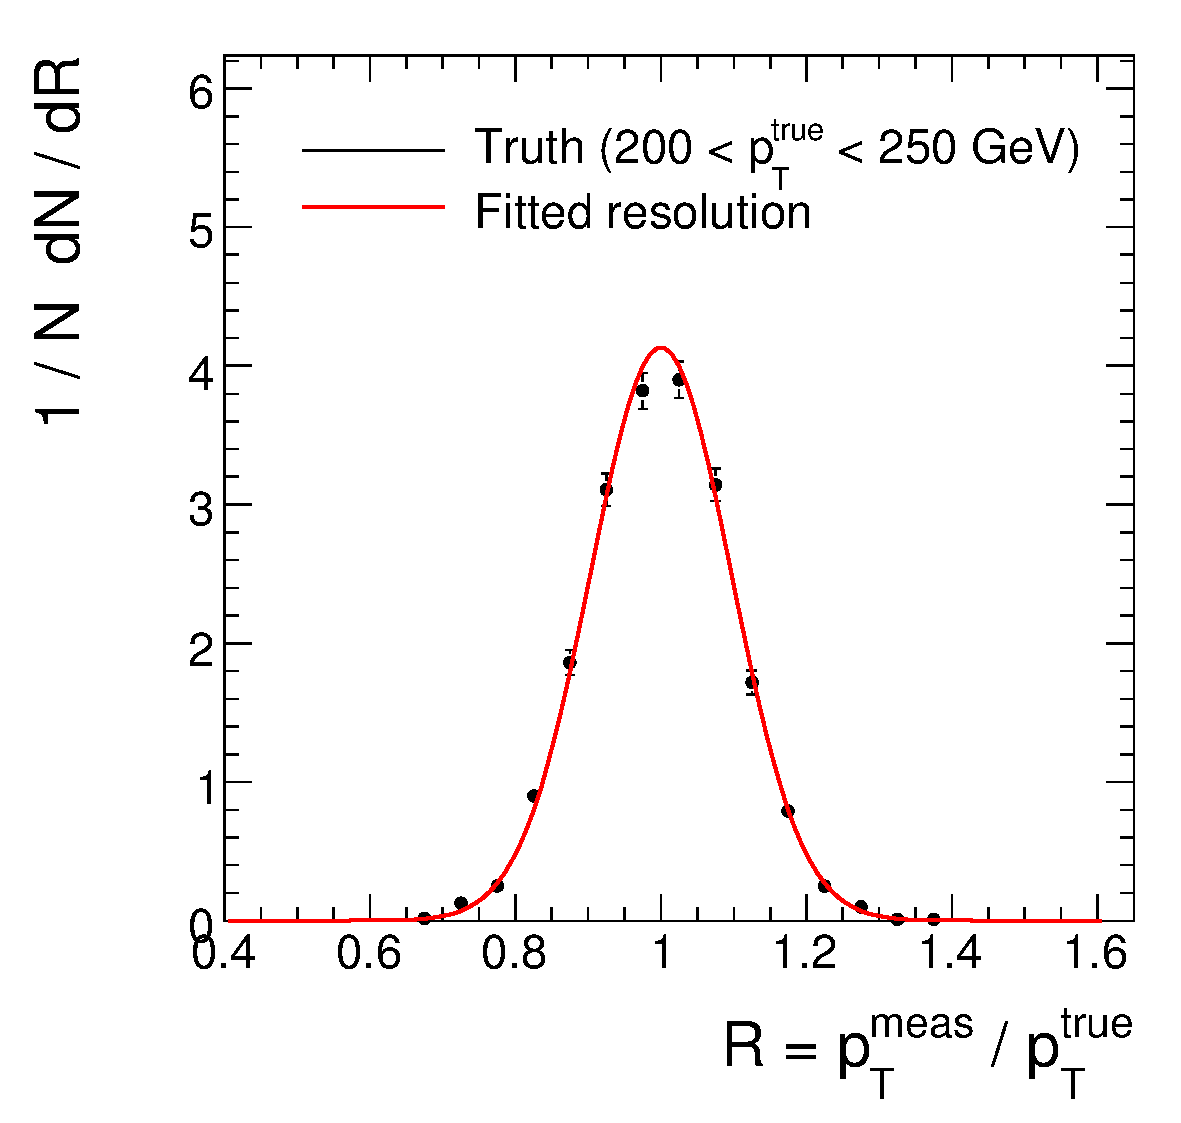
\includegraphics[width=0.45\textwidth]{figures/resFit_ToyMC_PtGenCuts_ResolutionBin7} \\      
    \end{tabular}
  \end{center}
  \caption{Simple simulation of a sample of ideal dijet events.
    Generated true response \mbox{$\ptmeas / \pttrue$} (histogram) and
    the response (solid line) from the maximum likelihood fit in two
    different \pttrue bins.
    The latter has been evaluated for the mean \pttrue in these bins.
    Note, here ``fit'' does not refer to a fit to the shown histogram but the maximisation of the likelihood~\eqref{eq:ResFit:Likelihood}.
  }
  \label{fig:ResFit:ToyMC:PtGenCuts:Response}
\end{figure}


\begin{table}[ht]
  \caption{Parameter values of the Gaussian jet \pt resolution
    $\sigma$.
    Listed are the true values used for the generation and
    the fitted values.
    The uncertainties assigned to the fitted values
    are the statistical uncertainties from the fit.
    The parameter correlations are shown in Fig.~\ref{fig:ResFit:ToyMC:PtGenCuts:ParCorr}.}
  \begin{center}
    \begin{tabular}[ht]{lccc}
      \toprule
      $\xi_{i}$ & $0$ & $1$ & $2$ \\
      \midrule
      True value & $4$           & $1.2$           & $0.05$ \\
      Fit result & $4.5 \pm 0.7$ & $1.18 \pm 0.05$ & $0.051 \pm 0.004$ \\
      \bottomrule
    \end{tabular}
  \end{center}
 \label{tab:ResFit:ToyMC:PtGenCuts:FitResult}
\end{table}


\begin{figure}[ht]
  \centering
  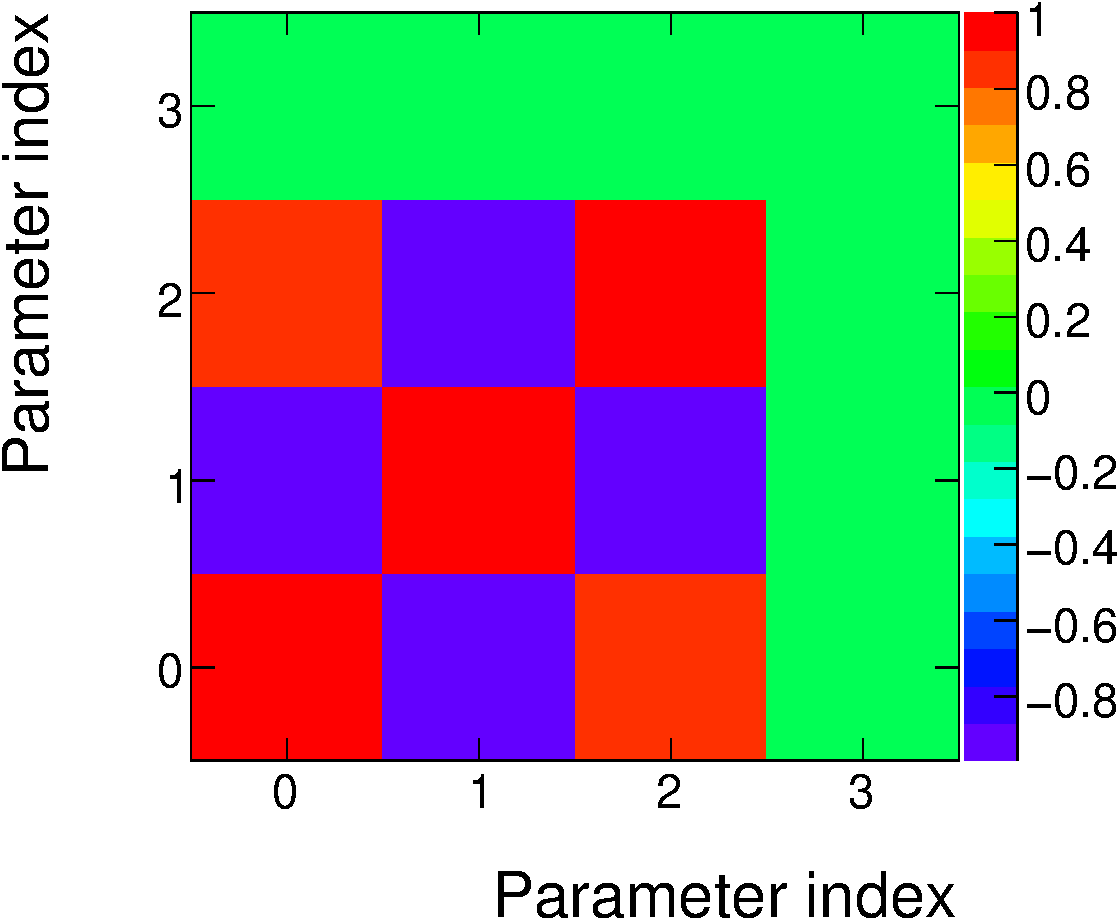
\includegraphics[width=0.45\textwidth]{figures/resFit_ToyMC_PtGenCuts_Correlations}
  \caption{Correlation coefficients of the fitted parameter values
    $\mathbf{\xi}$ of the Gaussian jet \pt resolution $\sigma$. 
    Parameter $3$ corresponds to the slope $\tau$ of the
    spectrum, which is fixed during the fit, and is to be ignored.}
  \label{fig:ResFit:ToyMC:PtGenCuts:ParCorr}
\end{figure}

The fitted parameter values $\mathbf{\xi}$ are listed in Tab.~\ref{tab:ResFit:ToyMC:PtGenCuts:FitResult};
they agree with the true values within the statistical uncertainties.

The parameters are strongly (anti-) correlated (comp. Fig.~\ref{fig:ResFit:ToyMC:PtGenCuts:ParCorr}).
In the present \pttrue interval from \mbox{$\ptmin = 50\gev$} to \mbox{$\ptmax = 1000\gev$}, the used parameterisation of the Gaussian resolution $\sigma$ is over-determined.
The $\xi_{0}$ term in~\eqref{eq:ResFit:ToyMC:Sigma} is most important at very low \pt while the $\xi_{2}$ term dominats at very large \pt.
Hence, omitting either the terms with $\xi_{0}$ and $\xi_{2}$ or the
term with $\xi_{1}$ would have been sufficient to describe the measured events.

\begin{figure}[ht]
  \begin{center}
    \begin{tabular}{cc}
     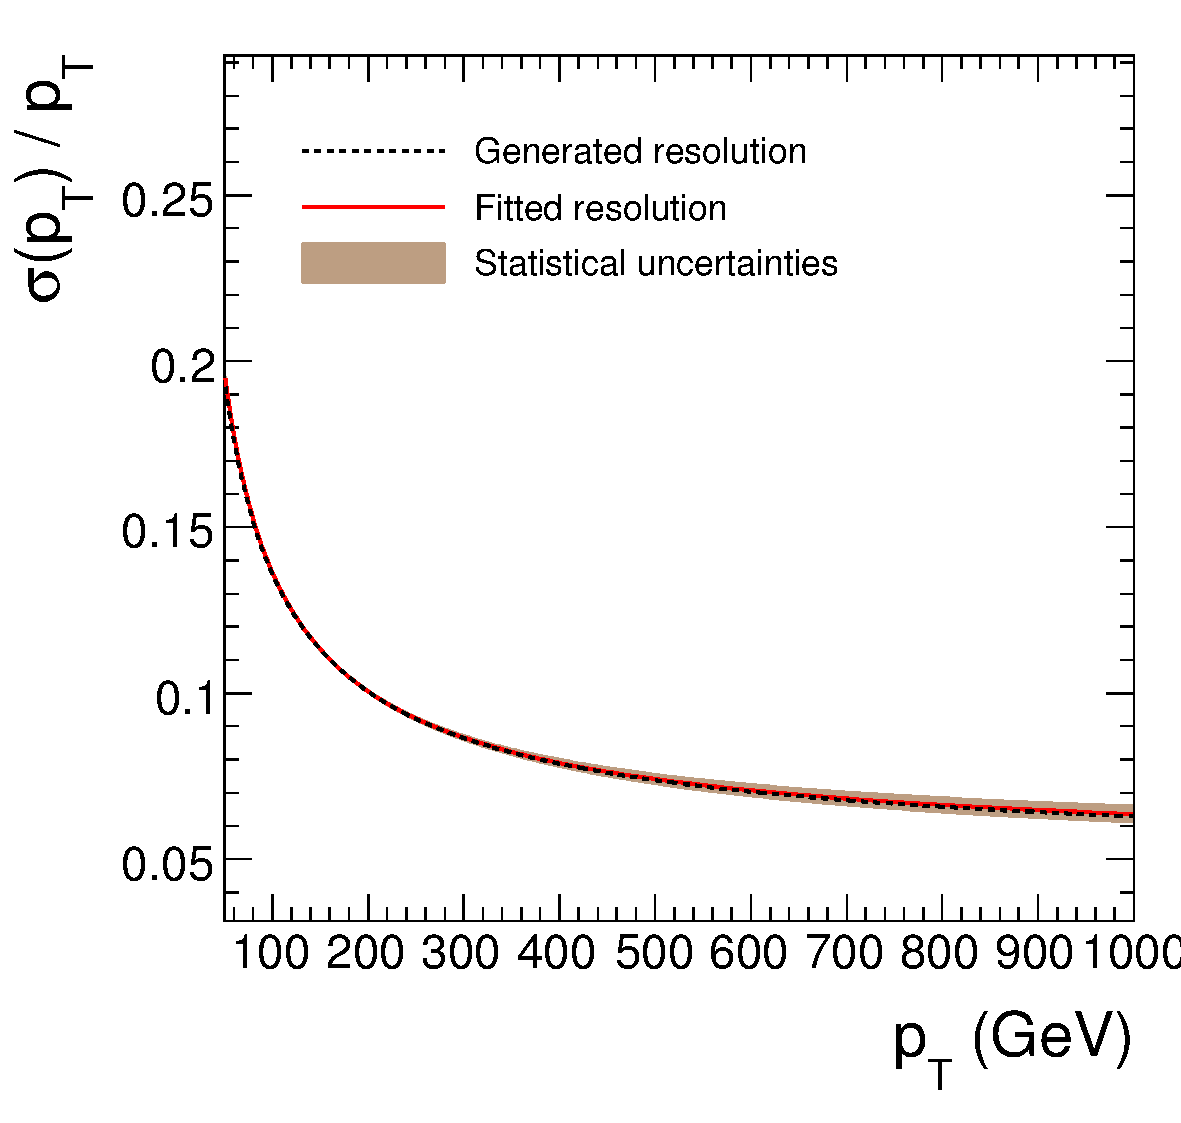
\includegraphics[width=0.45\textwidth]{figures/resFit_ToyMC_PtGenCuts_Sigma} &
     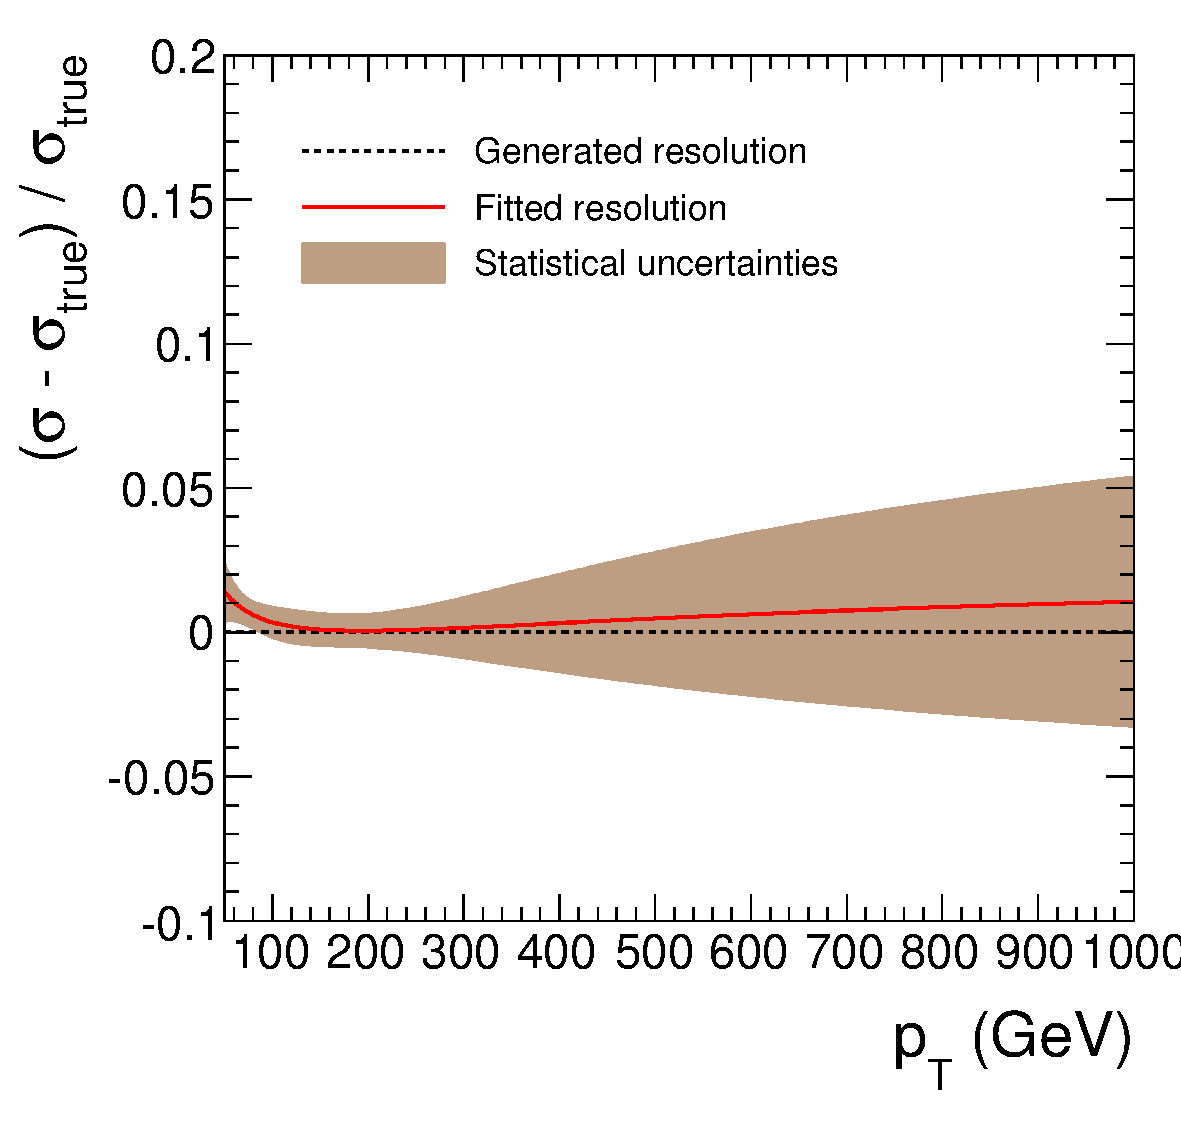
\includegraphics[width=0.45\textwidth]{figures/resFit_ToyMC_PtGenCuts_SigmaRelDifference} \\
   \end{tabular}
 \end{center}
  \caption{(\textit{Left}) Relative Gaussian resolution $\sigma(\pt)/\pt$ evaluated with the fitted
    parameter values (solid line) in comparison to the true resolution
    (dashed line) and (\textit{right}) the relative difference
    $\sigma_{\text{fit}} / \sigma_{\text{true}}$.
    The shaded areas represent the propagated statistical
    uncertainty on the fitted parameter values, taking into account the
    parameter correlations.}
  \label{fig:ResFit:ToyMC:PtGenCuts:FittedSigma}
\end{figure}

The Gaussian resolution $\sigma(\pt)/\pt$ evaluated with the fitted
parameter values is shown in Fig.~\ref{fig:ResFit:ToyMC:PtGenCuts:FittedSigma}
in comparison to the true width at generation.
There is good agreement between the fitted and the true resolution.
The uncertainties are about $1\%$ at low \pt rising to
about $3\%$ at $\pt \approx 600\gev$ where there is sufficient statistics in
the generated sample (comp. Fig~\ref{fig:ResFit:ToyMC:Sample:Spectrum}).
For larger \pt the uncertainties rise up to $4.5\%$.

An example of the resulting response distribution in comparison to the true
distribution is shown in Fig.~\ref{fig:ResFit:ToyMC:PtGenCuts:Response} for
two different \pttrue bins.


\subsection{Measurement of the resolution with a data driven event
  selection}\label{sec:ResFit:ToyMC:PtCaloCuts}

The modification of the maximum likelihood method for a data driven
event selection discussed in Section~\ref{sec:ResFit:Method:Biases} is
tested using the Toy Monte Carlo simulation.
Events are selected by requiring the measured \pt of the
first\footnote{This is that one jet of the two leading jets the
  selection requirement is placed on, i.e. not necessarily the leading
  jet (comp. Section~\ref{sec:ResFit:Method:Biases}).} jet to
meet \mbox{$\ptmin = 80 < \ptmeasi{1} < \ptmax = 800\gev$} (comp. Fig.~\ref{fig:ResFit:ToyMC:PtCuts:Spectrum}).

\begin{figure}[ht]
  \begin{center}
    \begin{tabular}{cc}
     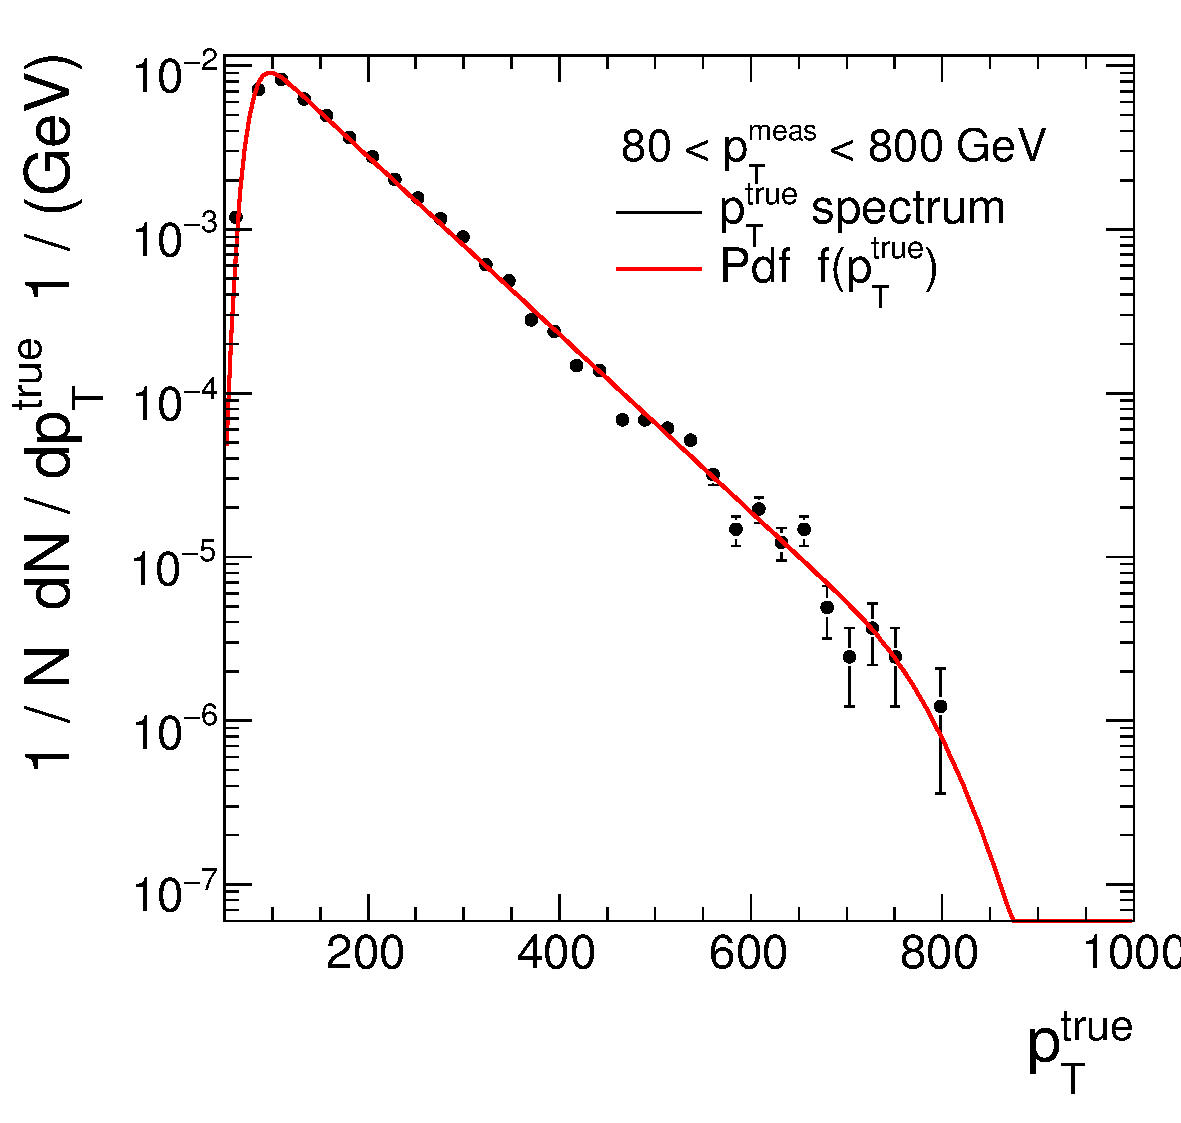
\includegraphics[width=0.45\textwidth]{figures/resFit_ToyMC_PtCuts_SpectrumLog} &
     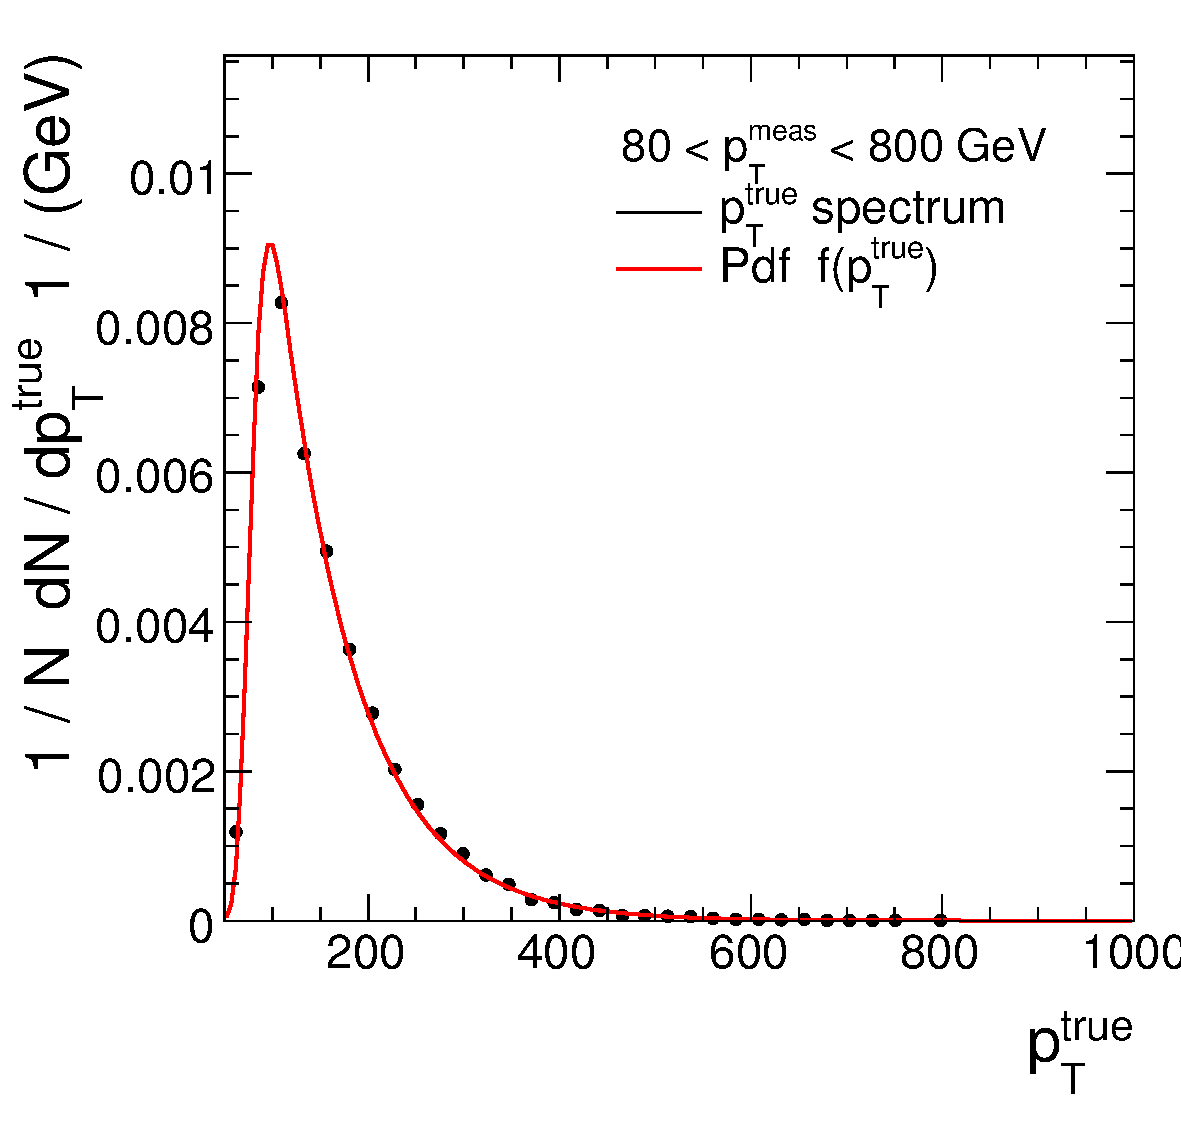
\includegraphics[width=0.45\textwidth]{figures/resFit_ToyMC_PtCuts_SpectrumLinear} \\
   \end{tabular}
 \end{center}
  \caption{Demonstration of the migration effects caused by a data
    driven event selection.
    Shown is the \pttrue spectrum (circular markers) after
    requiring \mbox{$80 < \ptmeas < 800\gev$}, in linear scale
    (\textit{left}) and logarithmic scale scale (\textit{right}).
    The spectrum is well described by the modified pdf
    $\tilde{f}(\pttrue)$.
    (Compare the underlying spectrum Fig.~\ref{fig:ResFit:ToyMC:Sample:Spectrum}.)
  }
  \label{fig:ResFit:ToyMC:PtCuts:Spectrum}
\end{figure}


\begin{figure}[ht]
  \begin{center}
    \begin{tabular}{cc}
     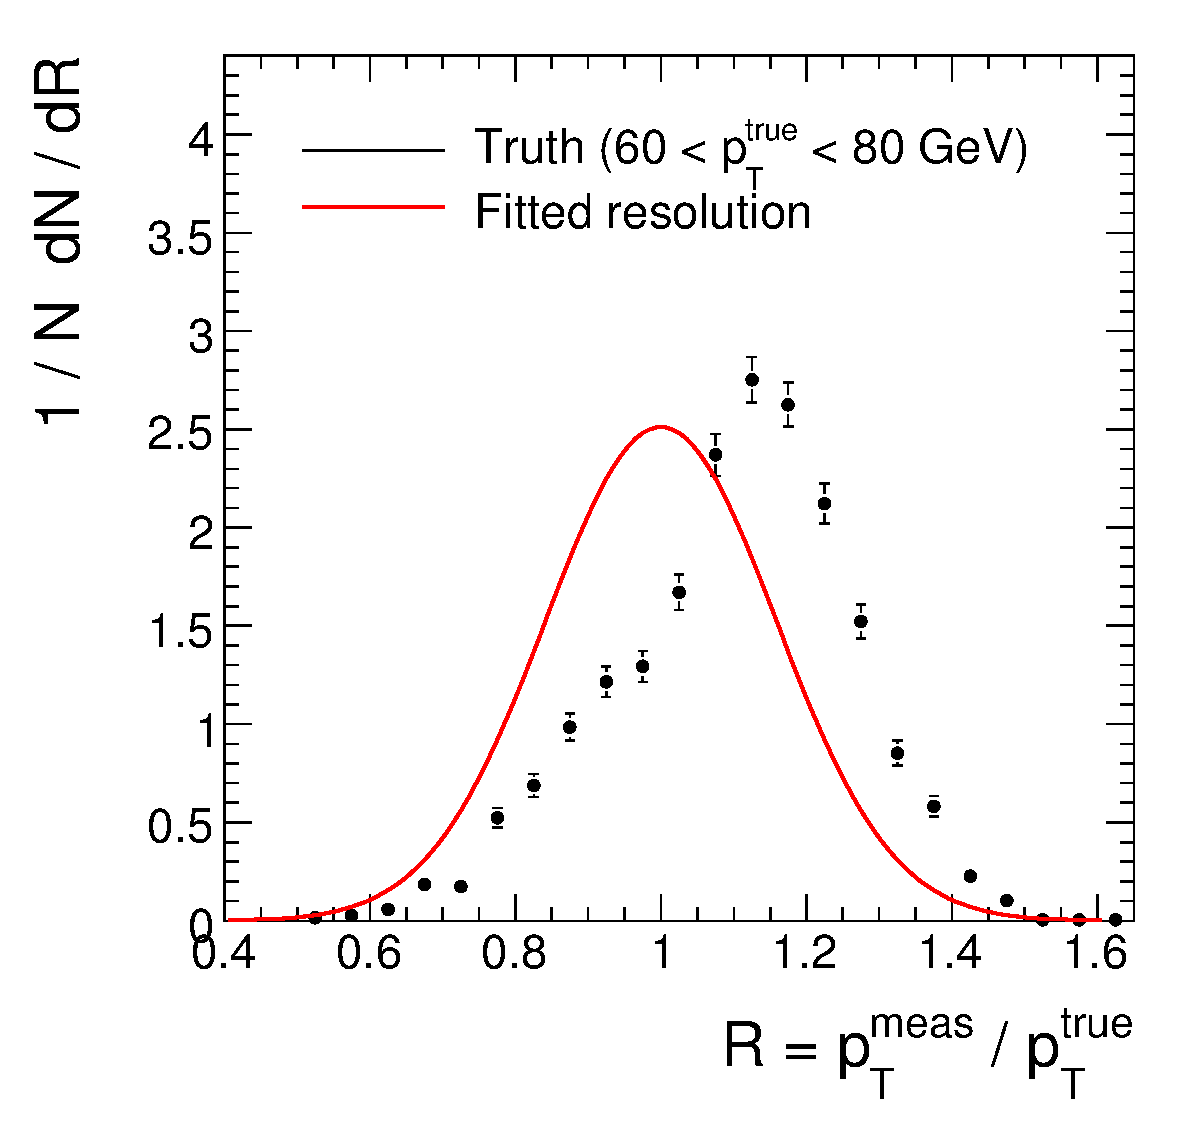
\includegraphics[width=0.45\textwidth]{figures/resFit_ToyMC_PtCuts_ResolutionBin1} &
     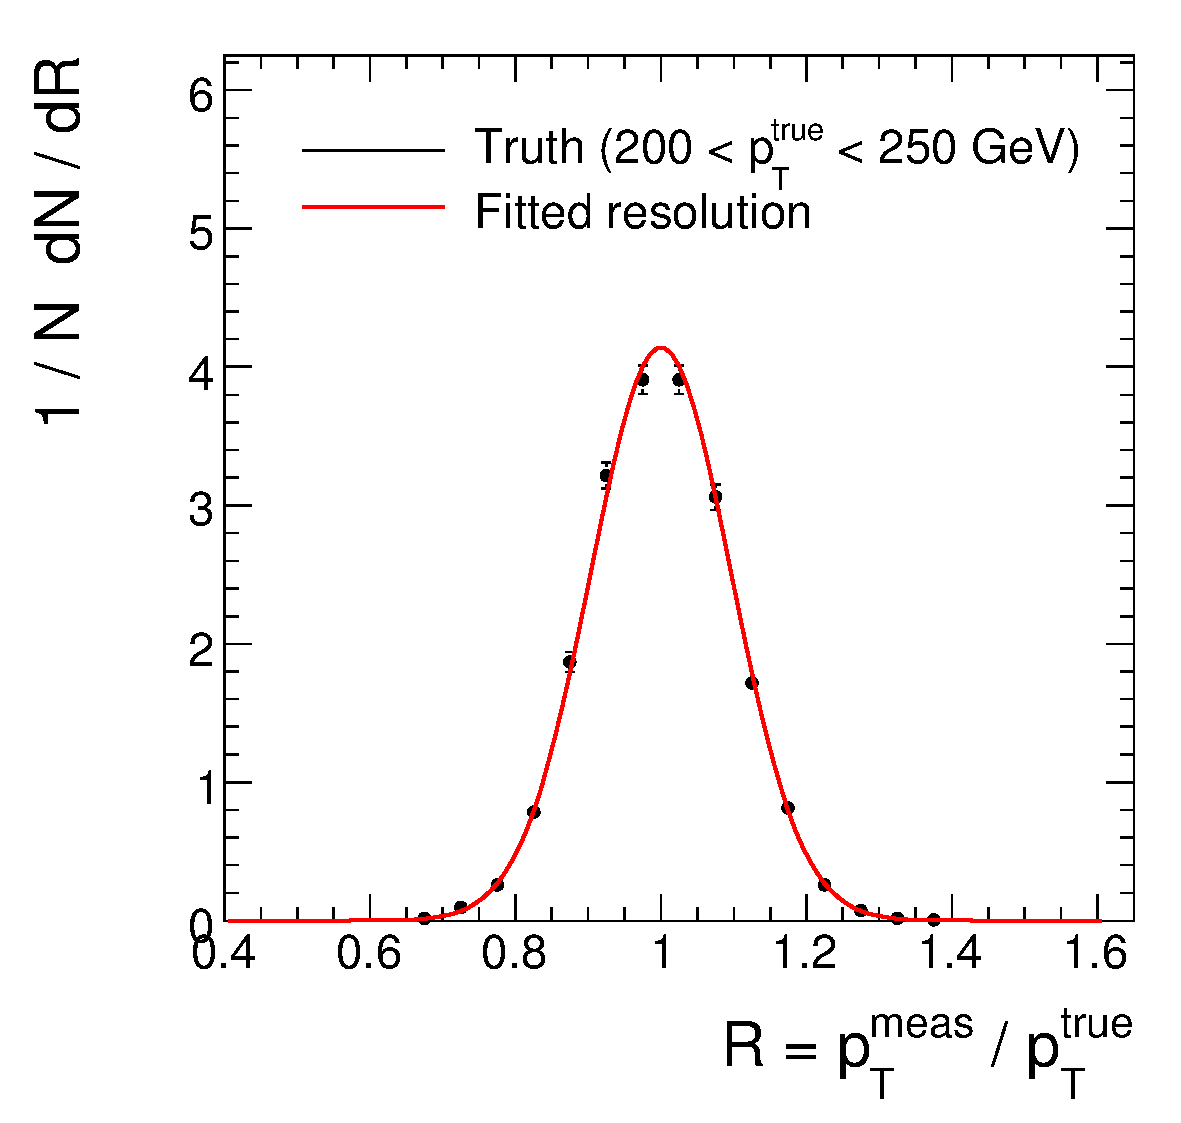
\includegraphics[width=0.45\textwidth]{figures/resFit_ToyMC_PtCuts_ResolutionBin7} \\
   \end{tabular}
 \end{center}
  \caption{Generated Gaussian response \mbox{$\ptmeas / \pttrue$}
    (circular markers) and the fitted
    response (solid line) in two different \pttrue bins after
    requiring \mbox{$80 < \ptmeas < 800\gev$}.
    Note the migration effects (\textit{left}): the narrow peak at the
    right side is populated by the first jets in each event, i.e. that have been cut on, and hence these are jets fluctuating upwards into the \pt bin.
    The wider peak centered around 1 is populated by the unconstrained
    second jet.
    (There is more upward than downward fluctuation due to the falling
    \pttrue spectrum.)
  }
  \label{fig:ResFit:ToyMC:PtCuts:Response}
\end{figure}

\begin{figure}[ht]
  \begin{center}
    \begin{tabular}{cc}
     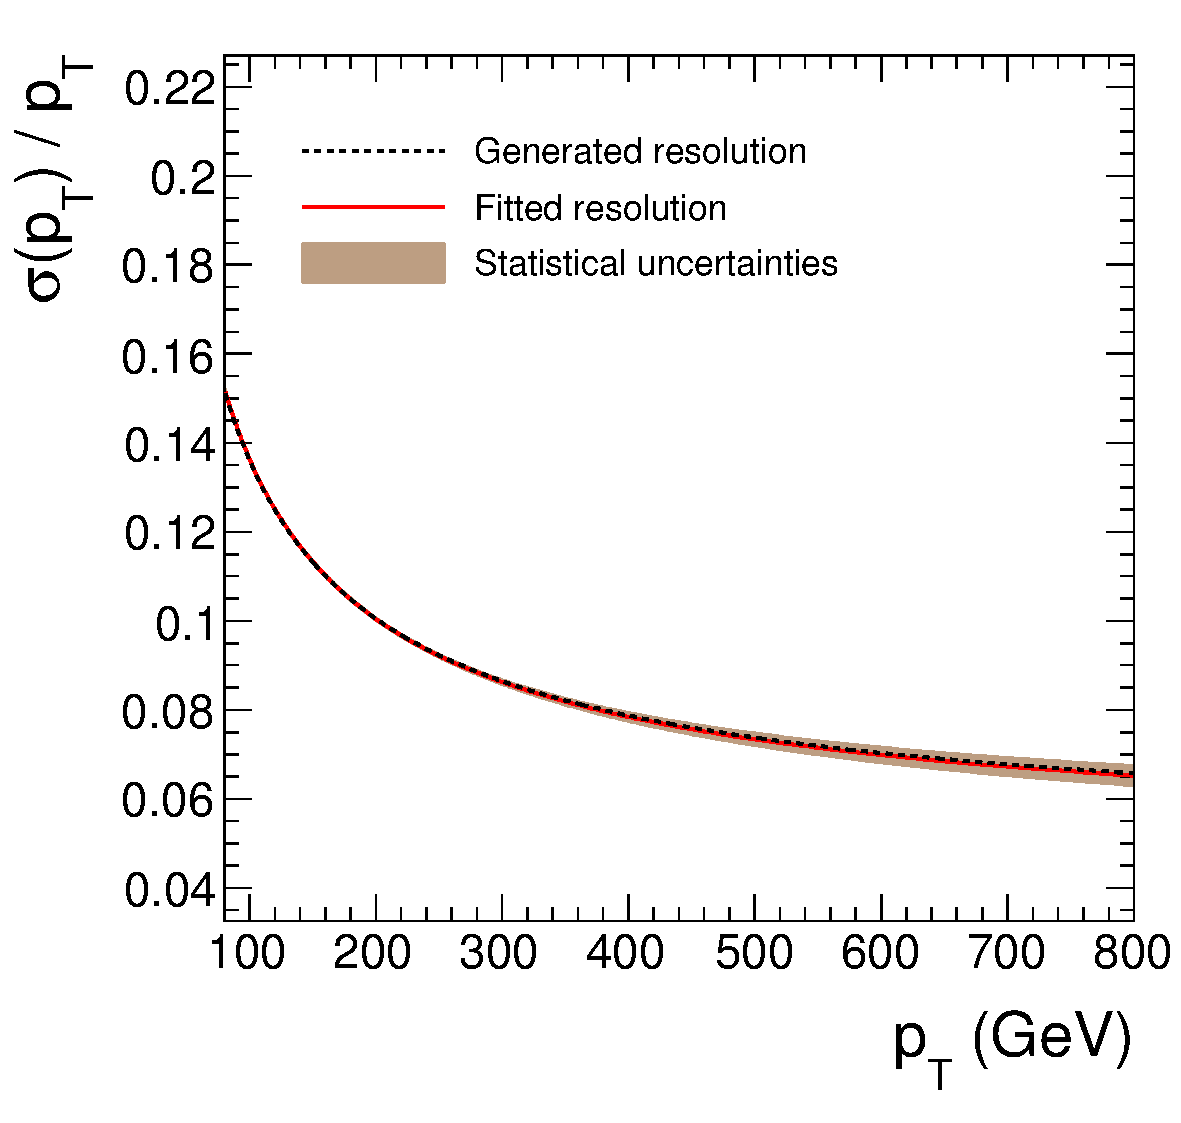
\includegraphics[width=0.45\textwidth]{figures/resFit_ToyMC_PtCuts_Sigma} &
     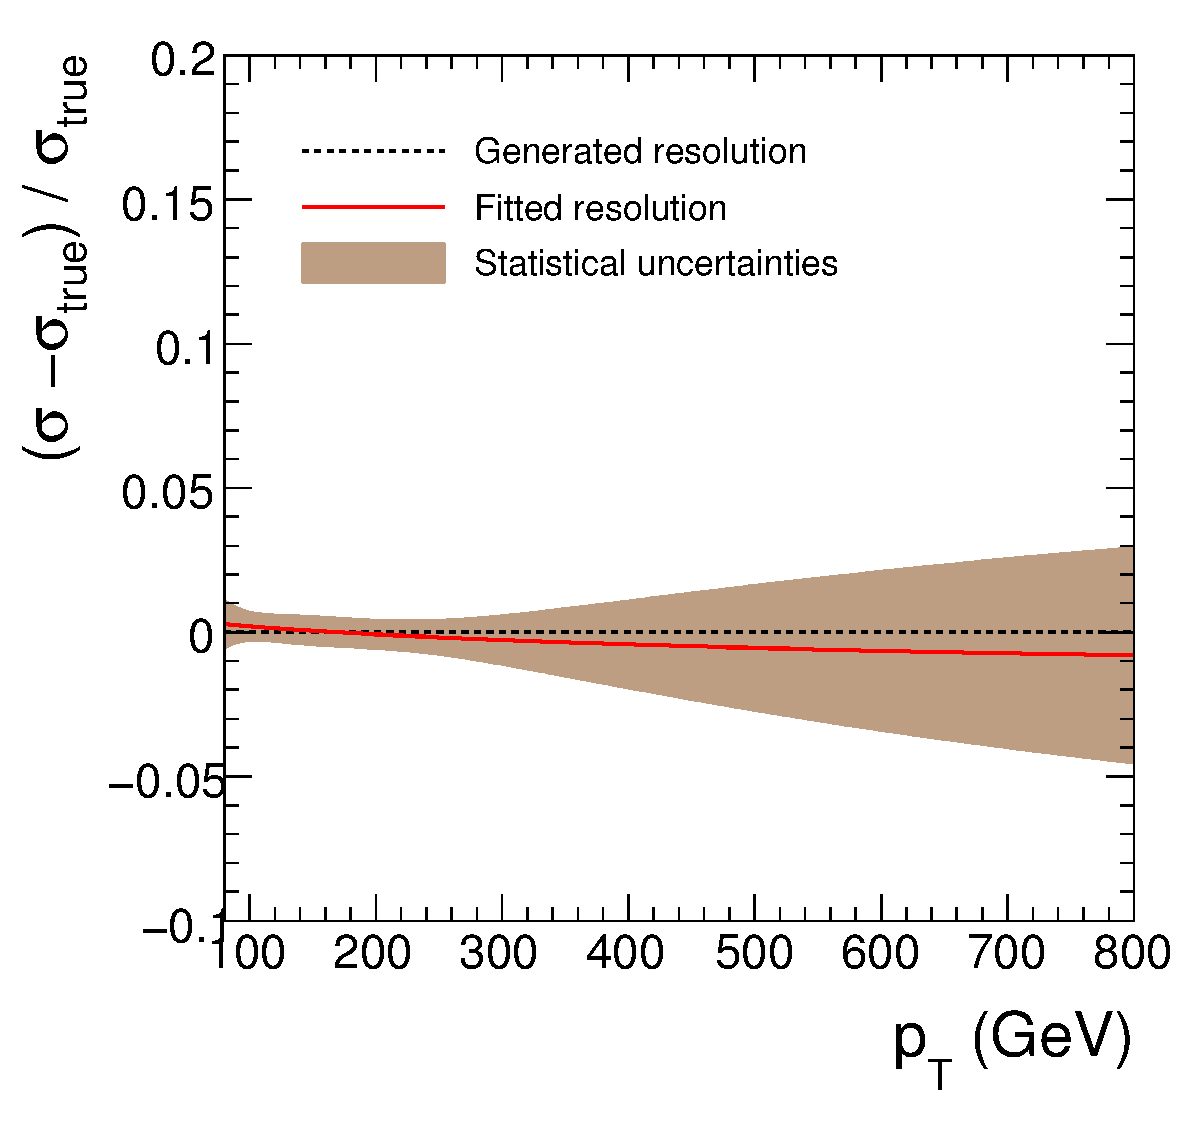
\includegraphics[width=0.45\textwidth]{figures/resFit_ToyMC_PtCuts_SigmaRelDifference} \\
   \end{tabular}
 \end{center}
  \caption{(\textit{Left}) Relative Gaussian resolution $\sigma(\pt)/\pt$ evaluated with the fitted
    parameter values (solid line) in comparison to the true resolution
    (dashed line) and (\textit{right}) the relative difference
    $\sigma_{\text{fit}} / \sigma_{\text{true}}$.
    The shaded areas represent the propagated statistical
    uncertainty on the fitted parameter values, taking into account the
    parameter correlations.
    The fit has been performed with dijet events selected by requiring \mbox{$80 < \ptmeas < 800\gev$}.}
  \label{fig:ResFit:ToyMC:PtCuts:FittedSigma}
\end{figure}


\begin{table}[ht]
  \caption{Parameter values of the Gaussian jet \pt resolution
    $\sigma$.
    Listed are the true values used for the generation and
    the fitted values.
    The uncertainties assigned to the fitted values
    are the statistical uncertainties from the fit.
    The fit has been performed with dijet events selected by requiring \mbox{$80 < \ptmeas < 800\gev$}.}
  \begin{center}
    \begin{tabular}[ht]{lccc}
      \toprule
      $b_{i}$ & $0$ & $1$ & $2$ \\
      \midrule
      True value & $4$           & $1.2$                   & $0.05$ \\
      Fit result   & $4 \pm 1$ & $1.20 \pm 0.07$ & $0.049 \pm 0.005$ \\
      \bottomrule
   \end{tabular}
  \end{center}
 \label{tab:ResFit:ToyMC:PtCuts:FitResult}
\end{table}


The fitted parameter values $\mathbf{\xi}$ of the Gaussian resolution $\sigma$ are listed in Tab.~\ref{tab:ResFit:ToyMC:PtCuts:FitResult}.
They agree with the true values within the statistical uncertainties.
As expected, they feature the same correlation pattern as in the
fitted parameters in Section~\ref{sec:ResFit:ToyMC:PtGenCuts}.

The relative Gaussian resolution $\sigma(\pt)/\pt$ evaluated with the fitted parameter values is shown in Fig.~\ref{sec:ResFit:ToyMC:PtGenCuts} in comparison to the true resolution at generation.
There is good agreement within the statistical uncertainties.
As before, the uncertainties are about $1\%$ at low \pt rising to about $3\%$ at $\pt \approx 600\gev$ and up to $4.5\%$ at very large \pt.
An example of the resulting response distributions is shown in
Fig.~\ref{fig:ResFit:ToyMC:PtCuts:Response} for two \pttrue bins.

From the results presented in this section, it is concluded that the
maximum likelihood method is suited to measure the jet \pt resolution
of dijets that are perfectly balanced in \pttrue.
% $Id: Note_ResFit_QCDMC.tex,v 1.1 2010/05/30 19:43:08 mschrode Exp $


\section{Study with a QCD Monte Carlo Simulation}\label{sec:ResFit:QCDMC}

The method is also tested on a sample of simulated QCD multijet events in $pp$ collisions at 7\tev center-of-mass energy.
They have been generated with PYTHIA and processed through the full CMS detector simulation application based on GEANT4\footnote{The used dataset is \texttt{/QCDFlat\_Pt15to3000/Spring10-START3X\_V26\_S09-v1/GEN-SIM-RECO}}.
The events are weighted corresponding to an integrated luminosity of 50\pbinv.


\subsection{Event selection}\label{sec:ResFit:QCDMC:EvtSel}

Jets are reconstructed from calorimeter towers using the anti-$k_{T}$ jet clustering algorithm~\cite{bib:akj} with parameter size $d=0.5$.
Jet energy corrections~\cite{bib:cmspas:jec} are applied to remove the $\eta$ and \pt dependence of the jet energy scale.
Dijet events are selected in the following way:
\begin{enumerate}
\item The third jet is required to have small \pt compared to the leading two jets by imposing \mbox{$\ptrel < x$}, with \mbox{$\ptrel = \frac{2\pti{3}}{\pti{1} + \pti{2}}$}, in order to ensure a dijet topology.
  The value of $x$ is varied in course of the analysis as discussed in Section~\ref{sec:ResFit:QCDMC:AddJetAct}.
\item Both leading jets are required to be in the same pseudorapidity bin, which are defined in Table~\ref{tab:ResFit:QCDMC:EtaBinning}.
  This accounts for the dependence of the jet \pt response on $\eta$ due to
  \begin{itemize}
  \item different calorimeter geometries and material budgets in front of the calorimeters in different pseudorapidity regions;
  \item the fact that the intrinsic calorimeter resolution is energy rather than \pt dependent.
  \end{itemize}
\item In order to reject jets clustered from noise in the hadronic calorimeter component, the fraction $f_{\text{em}}$ of energy deposited in the electromagnetic component is required to be \mbox{$f_{\text{em}} > 0.01$} for both leading jets~\cite{bib:cmspas:jetid}.
\end{enumerate}


\subsection{Gaussian resolution from Monte Carlo truth information}\label{sec:ResFit:QCDMC:MCTruthReso}

The jet \pt resolution is determined from Monte Carlo truth information, first, as a reference to compare the measured resolution to, and second, as an input $r_{0}$ in~\eqref{eq:ResFit:Method:ModifiedSpectrum} to incorporate the the selection bias into the dijet likelihood (comp. Section~\ref{sec:ResFit:Method:Biases}).
\begin{figure}[ht]
  \begin{center}
     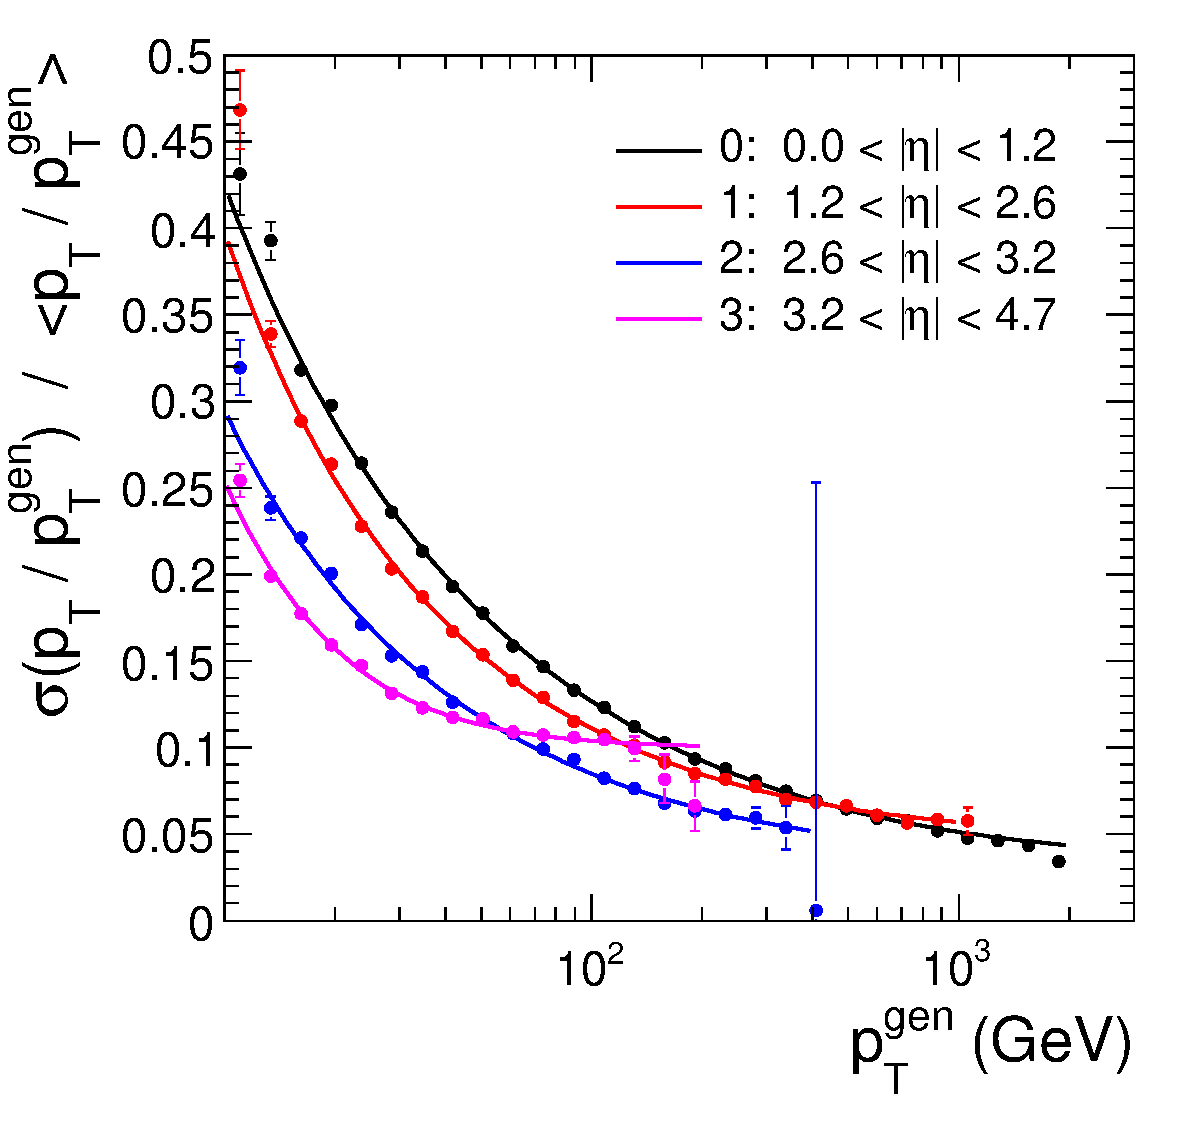
\includegraphics[width=0.45\textwidth]{figures/resFit_QCD_MCTruthResolution}
   \end{center}
   \caption{Relative Gaussian jet \pt resolution $\sigma/\pt$ derived from Monte Carlo truth as a function of \pt in different $\eta$ bins.}
   \label{fig:ResFit:ToyMC:Sample:Spectrum}
\end{figure}
The determination follows closely~\cite{}:
In each event, the two jets with highest particle level jet \pt, \ptparticle, are selected and the response distributions \mbox{$\ptmeas / \ptparticle$} are recorded in different bins of \ptparticle and $\eta$ (the $\eta$ binning is listed in Table~\ref{tab:ResFit:QCDMC:EtaBinning}).
The central part of each distribution --- defined by the interval of 1.5 standard deviations around the mean --- is fitted with a Gaussian.
In each $\eta$ bin, the fitted Gaussian widths $\sigma$ are interpolated for different \pt by the usual parametrisation function~\eqref{eq:ResFit:ToyMC:Sigma}; the fitted parameter values are listed in Table~\ref{tab:ResFit:QCDMC:MCTruthReso}.
\begin{table}[ht]
  \caption{Parameters of the MC truth resolution $\sigma$.}
  \begin{center}
    \begin{tabular}[h]{cccccc}
      \toprule
      & $|\eta_{\text{min}}|$ & $|\eta_{\text{max}}|$ & $\xi_{0}\,(\text{Ge}\kern-0.06667em\text{V})$ & $\xi_{1}\,(\sqrt{\text{Ge}\kern-0.06667em\text{V}})$ & $\xi_{2}$ \\
      \midrule
      $0$ & $0$ & $1.2$ & $1.9\pm0.2$ & $1.205\pm0.006$  & $0.0342\pm0.0007$ \\
      $1$ & $1.2$ & $2.6$ & $2.51\pm0.09$ & $0.968\pm0.009$  & $0.0483\pm0.0009$ \\
      $2$ & $2.6$ & $3.2$ & $1.7\pm0.18$ & $0.76\pm0.02$  & $0.035\pm0.004$ \\
      $3$ & $3.2$ & $4.7$ & $2.2\pm0.1$ & $0.2\pm0.1$  & $0.099\pm0.003$ \\
      \bottomrule
    \end{tabular}
  \end{center}
  \label{tab:ResFit:QCDMC:MCTruthReso}
\end{table}




\subsection{Effects from additional jet activity}\label{sec:ResFit:QCDMC:AddJetAct}

% Resolutions are derived from Gaussian fits to the simulated distributions~\eqref{eq:qcd:resolMaxlike:toyMCRes}.
% Figure.~\ref{fig:qcd:resolMaxlike:qcd:ptDependentSigma} illustrates on the lack of closure due to the presence of a third jet. 

% \begin{figure}[ht]
%   \begin{center}
%     \subfigure[]{
%       \includegraphics[width=0.45\textwidth]{figures/figures_QCD_resol_maxlike/resFit_PtDependentSigma}
%     } \subfigure[]{
%       \includegraphics[width=0.45\textwidth]{figures/figures_QCD_resol_maxlike/resFit_QCD_3rdJetInfluence}
%     }
%   \end{center}
%   \caption{(a) Gaussian jet \pt resolution in realistic jet
% events generated with PYTHIA and processed through the CMS full simulation
% application based on GEANT.
% $\sigma$ from fitted parameter values (red line) is compared to the MC truth prediction (blue line).
% (This is the result of a study on the \texttt{/QCDFlat\_Pt15to3000/Summer09-MC\_31X\_V9\_7TeV-v1/GEN-SIM-RECO} dataset. It will be updated to the Spring10 simulation but the differences are expected to be negligible.)
% (b) Illustration using a toy simulation of the effect of three jet events on the fitted 
% $\sigma$.}
%       \label{fig:qcd:resolMaxlike:qcd:ptDependentSigma}
% \end{figure}


% \begin{figure}[ht]
%   \centering
%   \includegraphics[width=0.45\textwidth]{figures/resFit_PtDependentSigma}
%   \caption{Width $\sigma$ of a Gaussian resolution in QCD dijet events. Shown is $\sigma$ from fitted parameter values (red line) in comparison to the truth from the MC simulation (blue line).}
%   \label{fig:resFit:qcd:ptDependentSigma}
% \end{figure}

% The determination of a Gaussian resolution~\eqref{eq:resFit:toyMCRes} with a \pt dependent width $\sigma$ as in~\eqref{eq:resFit:toyMCSigma} has been performed as for the ideal sample above.
% The results are not satisfying (comp. Fig.~\ref{fig:resFit:qcd:ptDependentSigma}).

% Various test have been performed and the method appears to work fine for a moderately falling \pt spectrum.
% In case of a realistic QCD spectrum (comp. Fig.~\ref{fig:resFit:qcd:dijetspectrum:subA}), however, the
% determined resolution does not describe the true resolution at large \pt anymore.
% The failure of the method is assumed to be due to the non-ideal topology of the selected dijet events, namely the presence of a third jet.
% These effects and an extension of the presented method are under study.
% Meanwhile a modified strategy to determine the resolution is investigated and presented in the following sections.

% $Id: Note_ResFit_QCDMC_Extrapolation.tex,v 1.2 2010/07/07 16:57:14 mschrode Exp $


\subsection{Extrapolation to the Two Jet Final State Topology}\label{sec:ResFit:QCDMC:Extrapolation}

As discussed in the previous Section~\ref{sec:ResFit:QCDMC:AddJetAct},
the presence of additional jets in the dijet event biases the
measurement towards larger resolutions and thus has to be corrected
for.
The size of the particle level jet \pt imbalance is correlated with the
measured relative \pt of the third jet as illustrated in Fig.~\ref{}.
Hence, in order to compensate for the bias in a data driven manner, different dijet samples with different maximal values $x$ of \ptrel (comp. step~1 of the event selection, Section~\ref{sec:ResFit:QCDMC:EvtSel}) are selected and the maximum likelihood fit is performed each time.
Then, the resulting resolution is extrapolated to the case of a two jet only event i.e. \mbox{$\ptrel\rightarrow0$}.

The approach chosen in the following is to define sufficiently small bins of jet \pt and measure the w.r.t. \pt average response in each bin for different limits \mbox{$\ptrel<x$}.
This is motivated by the fact that in case of a Gaussian response parametrisation (Section~\ref{sec:ResFit:QCDMC:Gauss}) there is then only one parameter $\bar{\sigma}$, which can be extrapolated relatively straight forward.
The chosen \pt and $\eta$ binning is listed in Table~\ref{tab:ResFit:QCDMC:Extrapolation:Binning}.
\begin{table}[ht]
  \caption{Definition of \pt bins for the fit of the mean Gaussian resolution.}
  \centering
  \begin{tabular}{cl|ccccccccc}
    \toprule
    \multicolumn{2}{c}{$|\eta|$ bin} & \multicolumn{9}{c}{\pt bin edges $(\text{Ge}\kern-0.06667em\text{V})$} \\
    \midrule
    \multirow{2}{*}{$0$} & \multirow{2}{*}{$(0 - 1.2)$} & 80 & 100 & 120 & 140 & 170 & 200 & 250 & 300 & 350 \\
    && 400 & 500 & 600 & 800 & 1000 \\
    $1$ & $(1.2 - 2.6)$ & 60 & 80 & 100 & 120 & 150 & 200 & 300 &  500 & 700 \\
    $2$ & $(2.6 - 3.2)$ & 80 & 100 & 150 &&&&&&\\
    \bottomrule
  \end{tabular}
  \label{tab:ResFit:QCDMC:Extrapolation:Binning}
\end{table}

Was the Gaussian parametrised with a \pt dependent $\sigma$ as e.g. in~\eqref{eq:ResFit:ToyMC:Sigma}, the correlation of the parameter $\xi_{i}$ of $\sigma$ would have to be taken into account in contrast.
Note that this is exactly the case for the Crystal Ball response parametrisation (Section~\ref{sec:ResFit:QCDMC:CrystalBall}), and additional work is forseen to uncorrelate the parameters $\sigma$, $\alpha$, and $n$.

In the following, the particle level differential dijet cross section is taken from the interpolated \ptparticle distribution Fig.~\ref{fig:ResFit:QCDMC:Extrapolation:Gauss:ExBin:SpectrumAndExtrapolation} (\textit{left}) that has been obtained from the Monte Carlo truth information. 



\subsubsection{Measurement of the Gaussian response function}\label{sec:ResFit:QCDMC:Gauss}

A sample of dijet events is selected for each $\eta$, \pt bin listed in Table~\ref{tab:ResFit:QCDMC:Extrapolation:Binning}.
The selection bias (Section~\ref{sec:ResFit:Method:Biases}) is incorporated in the probability densitity function as before, comp. Fig.~\ref{fig:ResFit:QCDMC:Extrapolation:Gauss:ExBin:SpectrumAndExtrapolation} (\textit{left}).

\begin{figure}[ht]
  \centering
  \begin{tabular}{cc}
    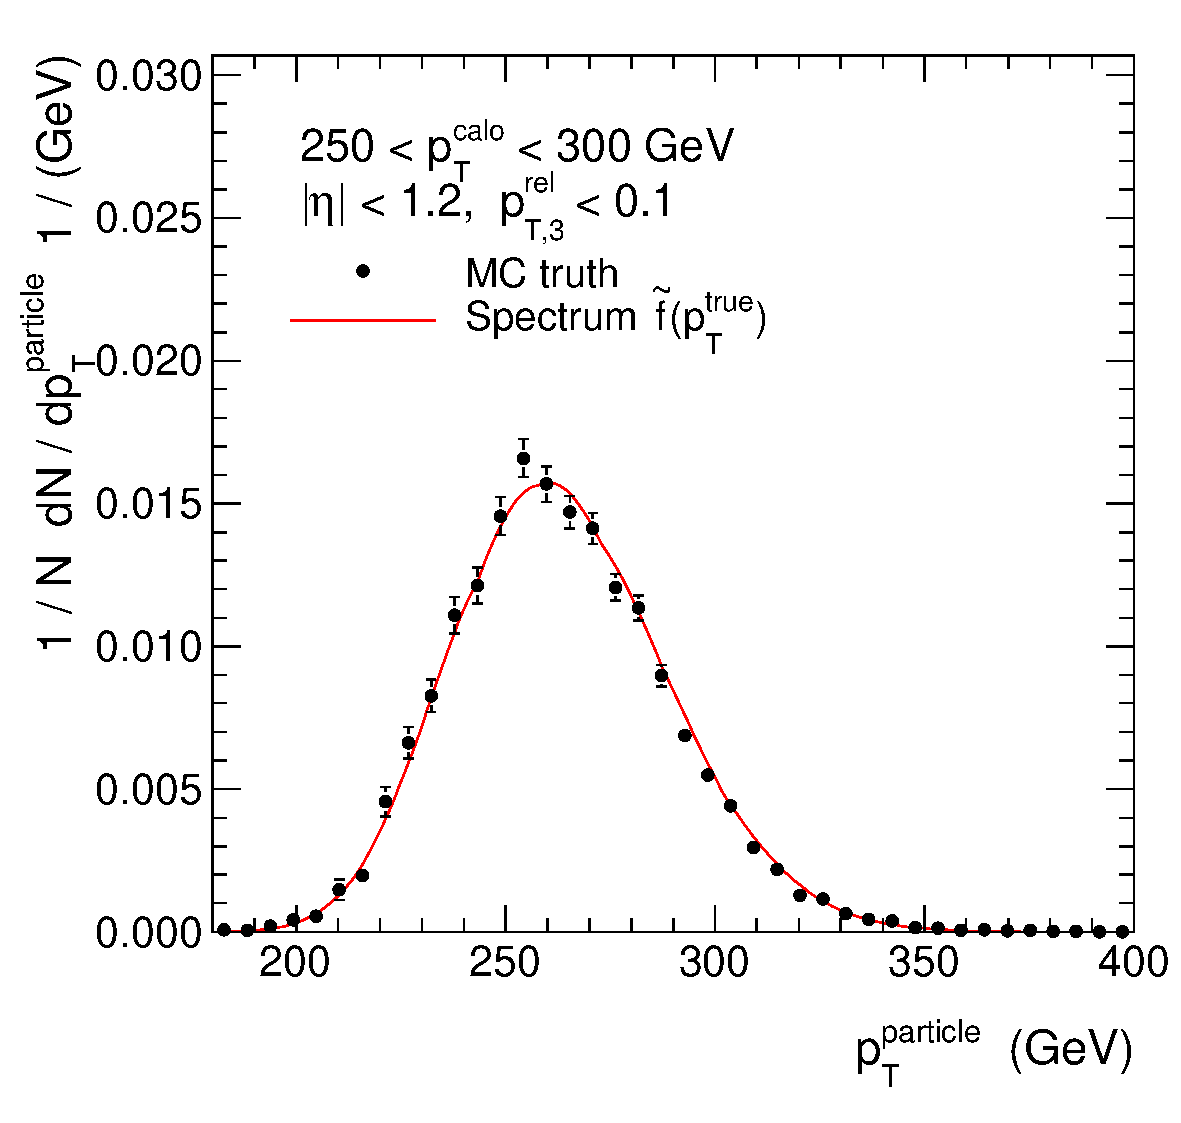
\includegraphics[width=0.45\textwidth]{figures/ResFit_Spring10QCDFlat_Gauss_Eta0_Spectrum_PtBin6} &
    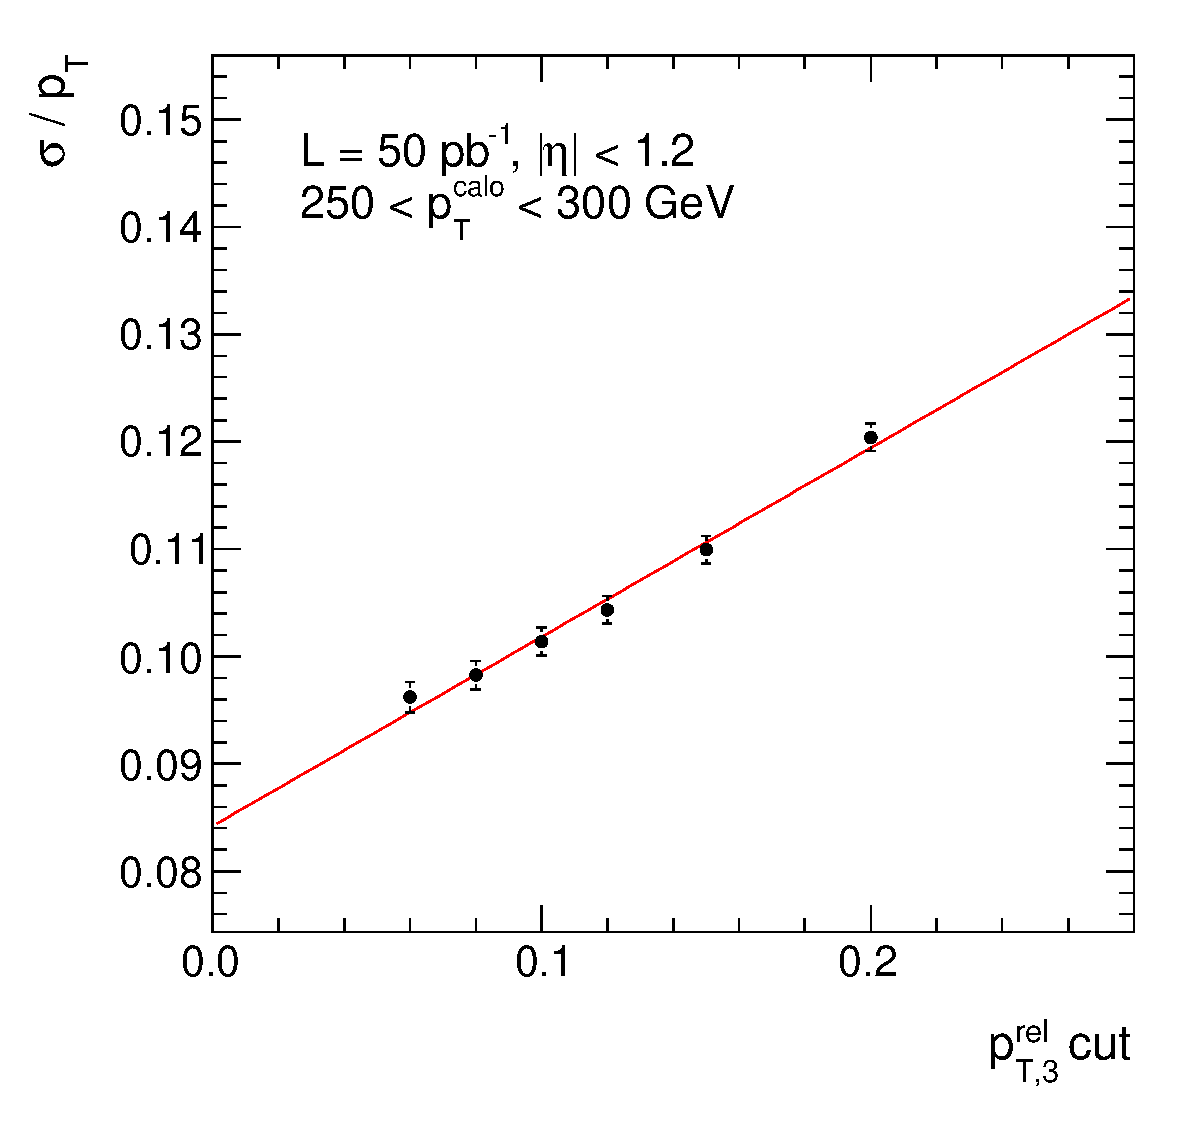
\includegraphics[width=0.45\textwidth]{figures/ResFit_Spring10QCDFlat_Gauss_Eta0_ExtrapolatedPar0_PtBin6}
  \end{tabular}
\caption{(\textit{Left}) The parameterisation of the realistic particle jet \pt spectrum in one \pt bin as used in the dijet likelihood (solid line) in comparison to the prediction from Monte Carlo truth (full circles). 
  (\textit{Right}) $\bar{\sigma}/\pt$ from Gaussian fits for different limits on \ptrel in the same \pt bin.
  The solid line is a linear fit to extrapolate $\bar{\sigma}/\pt$ to the ideal case of only two jets in the
  final state.}
\label{fig:ResFit:QCDMC:Extrapolation:Gauss:ExBin:SpectrumAndExtrapolation}
\end{figure}

The mean Gaussian response
\begin{equation*}
  r_{\mathbf{\bar{\sigma}}}\left(\ptmeas|\pttrue\right) = 
  \frac{1}{\sqrt{2\pi}\bar{\sigma}}\exp\left[-\frac{1}{2}\left(\frac{\ptmeas - \pttrue}{\bar{\sigma}}\right)^{2}\right]
\end{equation*}
is measured in each bin by maximising the likelihood~\eqref{eq:ResFit:Likelihood} w.r.t.~$\bar{\sigma}$.
The fitted relative Gaussian widths $\bar{\sigma}/\pt$ in one \pt bin are shown in Fig.~\ref{fig:ResFit:QCDMC:Extrapolation:Gauss:ExBin:SpectrumAndExtrapolation} (\textit{right}) for different limits on \ptrel.
Here, \pt is the mean value of the asssumed spectrum~$\tilde{f}(\pttrue)$ in that bin, shown Fig.~\ref{fig:ResFit:QCDMC:Extrapolation:Gauss:ExBin:SpectrumAndExtrapolation} (\textit{left}).
In order to extrapolate the measurements to the case of a two jet only event, the $\bar{\sigma}/\pt$ are fitted with a linear function --- shown as a solid line --- and the $y$ axis intercept is taken as the corrected jet \pt resolution.

The jet \pt spectra, fitted Gaussian resolutions $\bar{\sigma}/\pt$ versus \ptrel, and the extrapolation are shown in Appendix~\ref{sec:ResFit:App:Gauss:AllResults} for all \pt and $\eta$ bins.

\begin{figure}[ht]
  \centering
  \begin{tabular}{cc}
    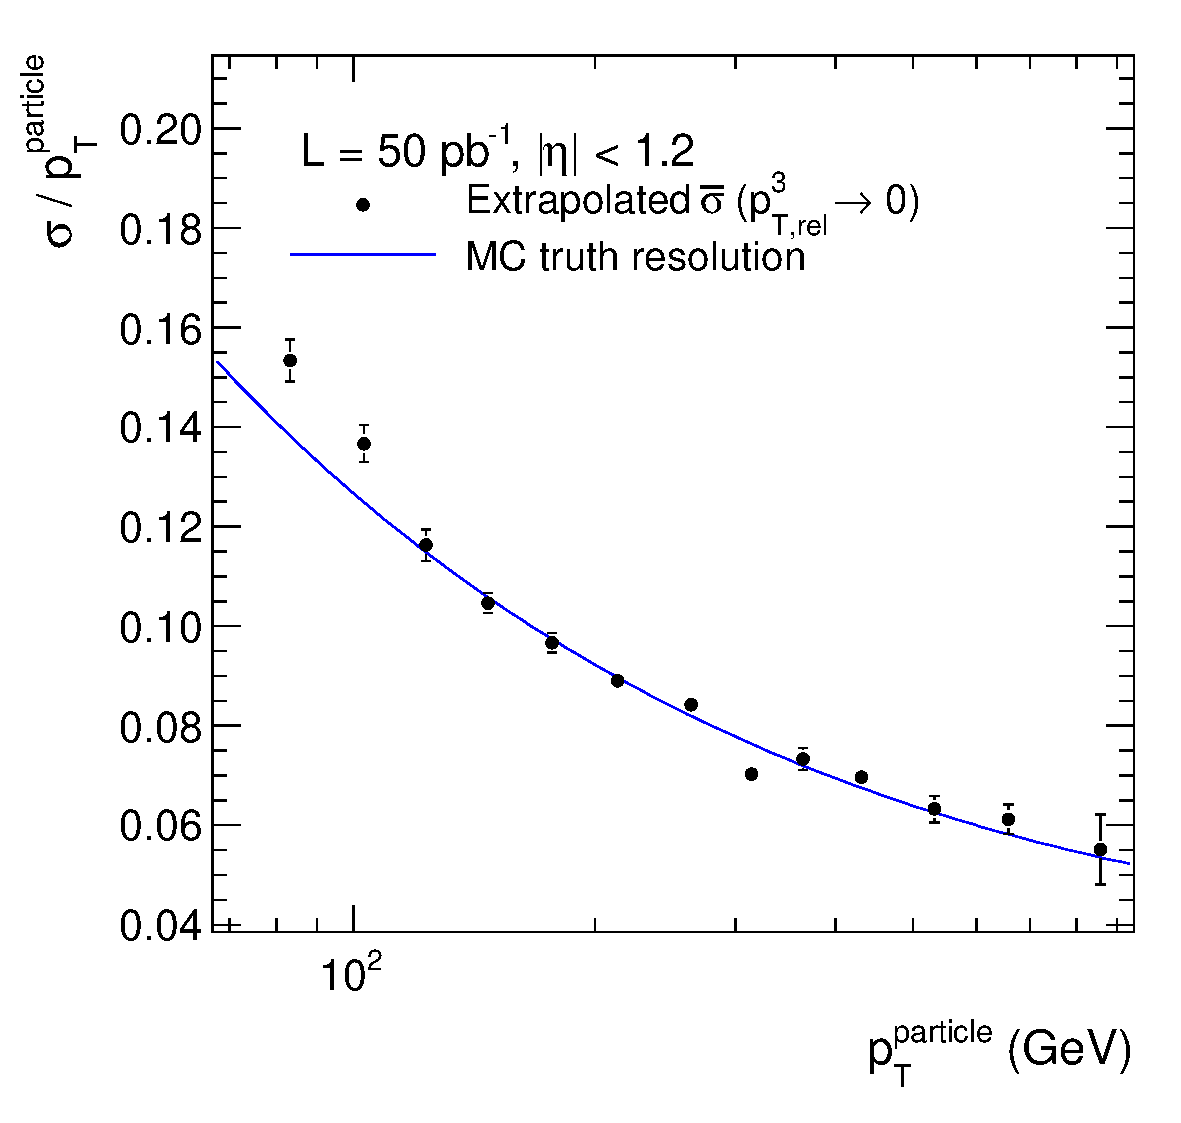
\includegraphics[width=0.45\textwidth]{figures/ResFit_Spring10QCDFlat_Gauss_Eta0_ExtrapolatedResolution} &
    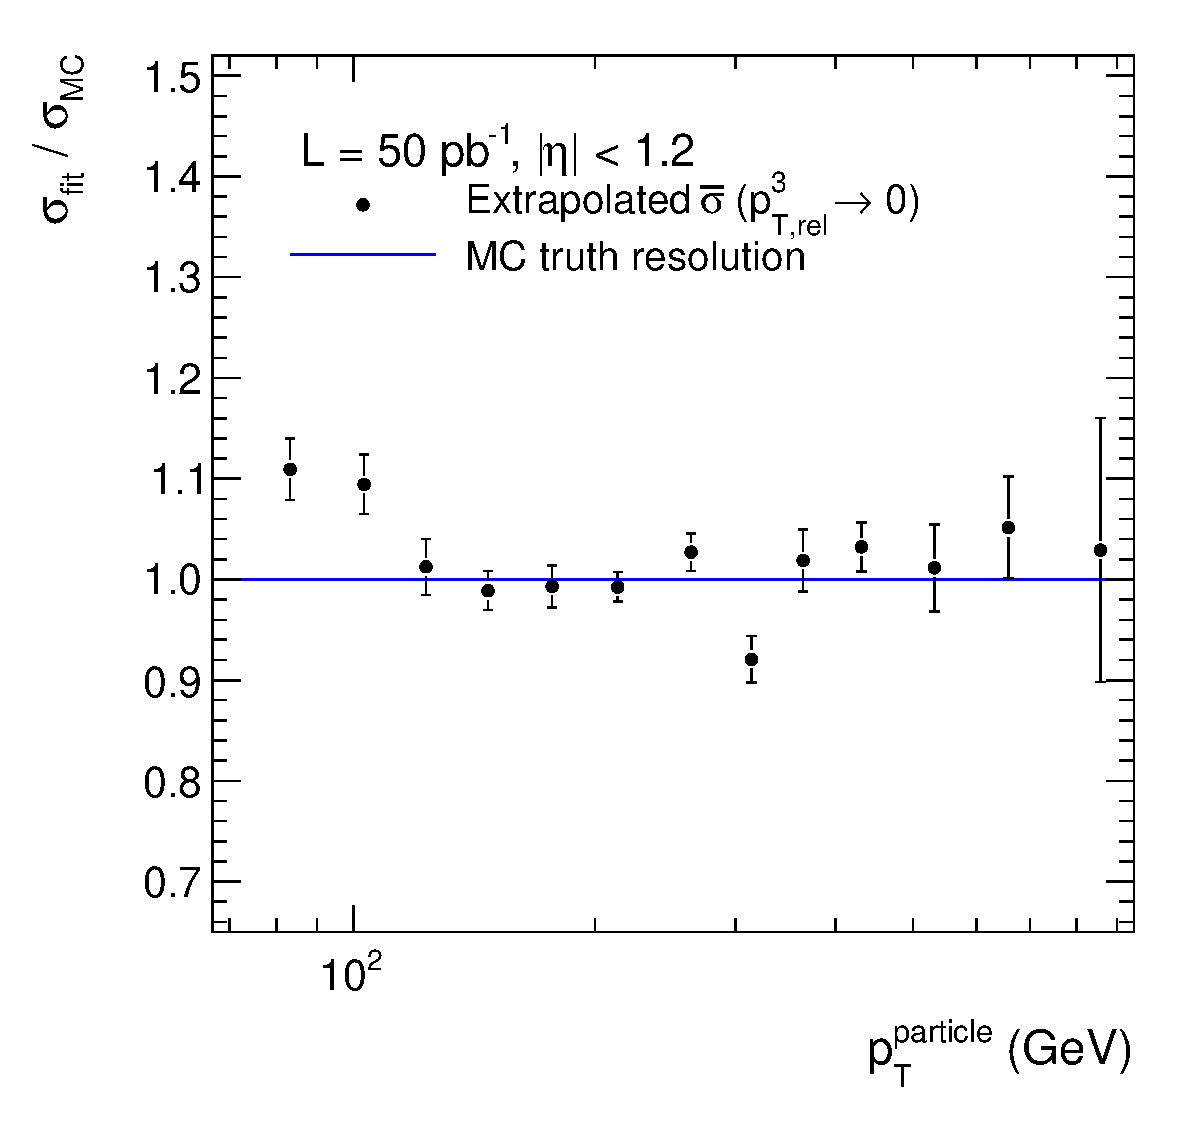
\includegraphics[width=0.45\textwidth]{figures/ResFit_Spring10QCDFlat_Gauss_Eta0_ExtrapolatedResolutionRatio}
  \end{tabular}
\caption{(\textit{Left}) Fitted Gaussian jet \pt resolutions, $\bar{\sigma}/\pt$, from extrapolations for \mbox{$\ptrel\rightarrow0$} in different \pt bins.
  The \pt are the mean values of $\tilde{f}(\pttrue)$ in each bin.
  The error bars indicate the combined statistical uncertainties from the extrapolation and the Monte Carlo statistics.
  The dashed line shows the Monte Calro truth resolution for comparison.
  (\textit{Right}) Ratio of fitted and Monte Carlo truth resolution.}
\label{fig:ResFit:QCDMC:Extrapolation:Gauss:ResoVsPt}
\end{figure}

The jet \pt resolution $\bar{\sigma}/\pt$ measurements, corrected for the effect of additional jet activity, are shown for different \pt bins in Fig.~\ref{fig:ResFit:QCDMC:Extrapolation:Gauss:ResoVsPt}.
(Again, the \pt are the mean values of the asssumed spectrum~$\tilde{f}(\pttrue)$ in each bin.)
The fitted values are in good agreement with the Monte Carlo truth prediction, shown as a dash line.
The larger deviation in the two low \pt bins is assumed to be caused by the increasing influence of incorrect jet ordering due to the greater resolution on the extrapolation procedure\footnote{This effect is seen when using the dijet asymmetry method to measure jet \pt resolutions~\cite{bib:cmspas:dijetasymm}.}.

The error bars shown in Fig.~\ref{fig:ResFit:QCDMC:Extrapolation:Gauss:ResoVsPt} represent the combined statistical uncertainties of the fit and due to the Monte Carlo sample size:
\begin{enumerate}
\item The first contribution is the statistical uncertainty on the parameter of $y$ axis intercept in the linear extrapolation (Fig.~\ref{fig:ResFit:QCDMC:Extrapolation:Gauss:ExBin:SpectrumAndExtrapolation} (\textit{left})).
\item The second contribution arises from the uncertainty due to the limited Monte Carlo sample size.
 As the event weights are large for small \pt, statistical fluctations become significant.
 In order to roughly evaluate this uncertainty, the same fits have been performed again without event weights (for the used sample this corresponds to a flattened QCD spectrum).
 The statistical uncertainties obtained in this case on the $y$ axis intercept are added in quadrature to the ones in 1.
 This procedure has to be improved to obtain a statistically correct description of the uncertainty.
\end{enumerate}

Due to the selection requirement \mbox{$\ptrel < x$}, all events selected for a particular value of $x$ in Fig.~\ref{fig:ResFit:QCDMC:Extrapolation:Gauss:ExBin:SpectrumAndExtrapolation} (\textit{right}) are also included in the samples selected with larger values of $x$.
Hence, the measured widths $\bar{\sigma}/\pt$ in one \pt are strongly correlated.
This correlation is not considered in the qouted uncertainties.
The planned treatment is to either include the correlations explicitly or performe the measurements in exclusive bins of \ptrel.

\begin{figure}[ht]
  \centering
    \begin{tabular}{ccc}
      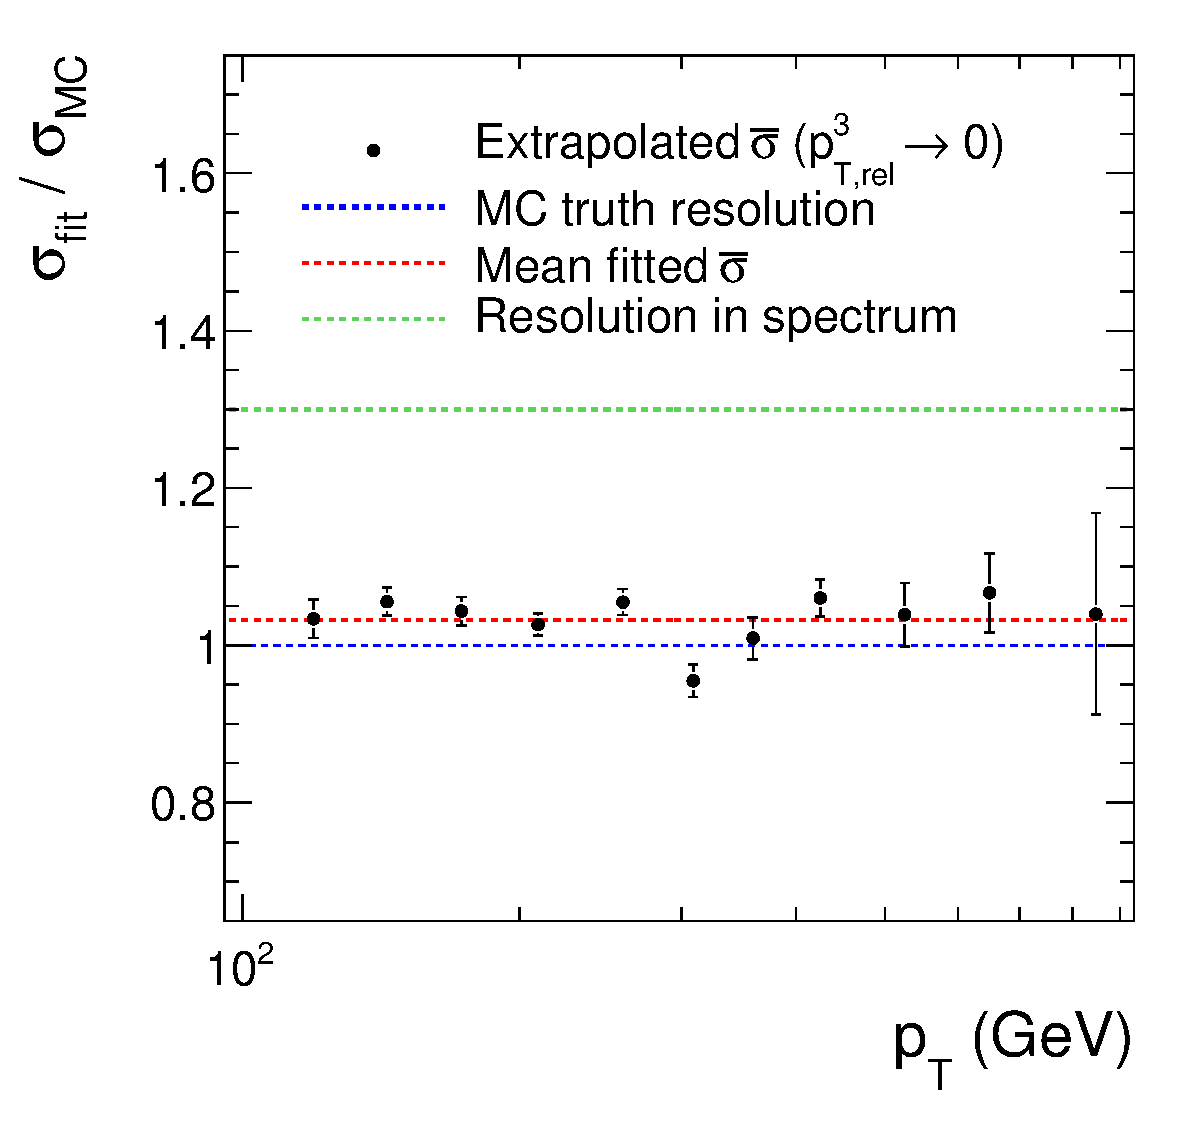
\includegraphics[width=0.3\textwidth]{figures/ResFit_Spring10QCDFlat_GaussUp30It0_Eta0_ExtrapolatedResolutionRatio} &
      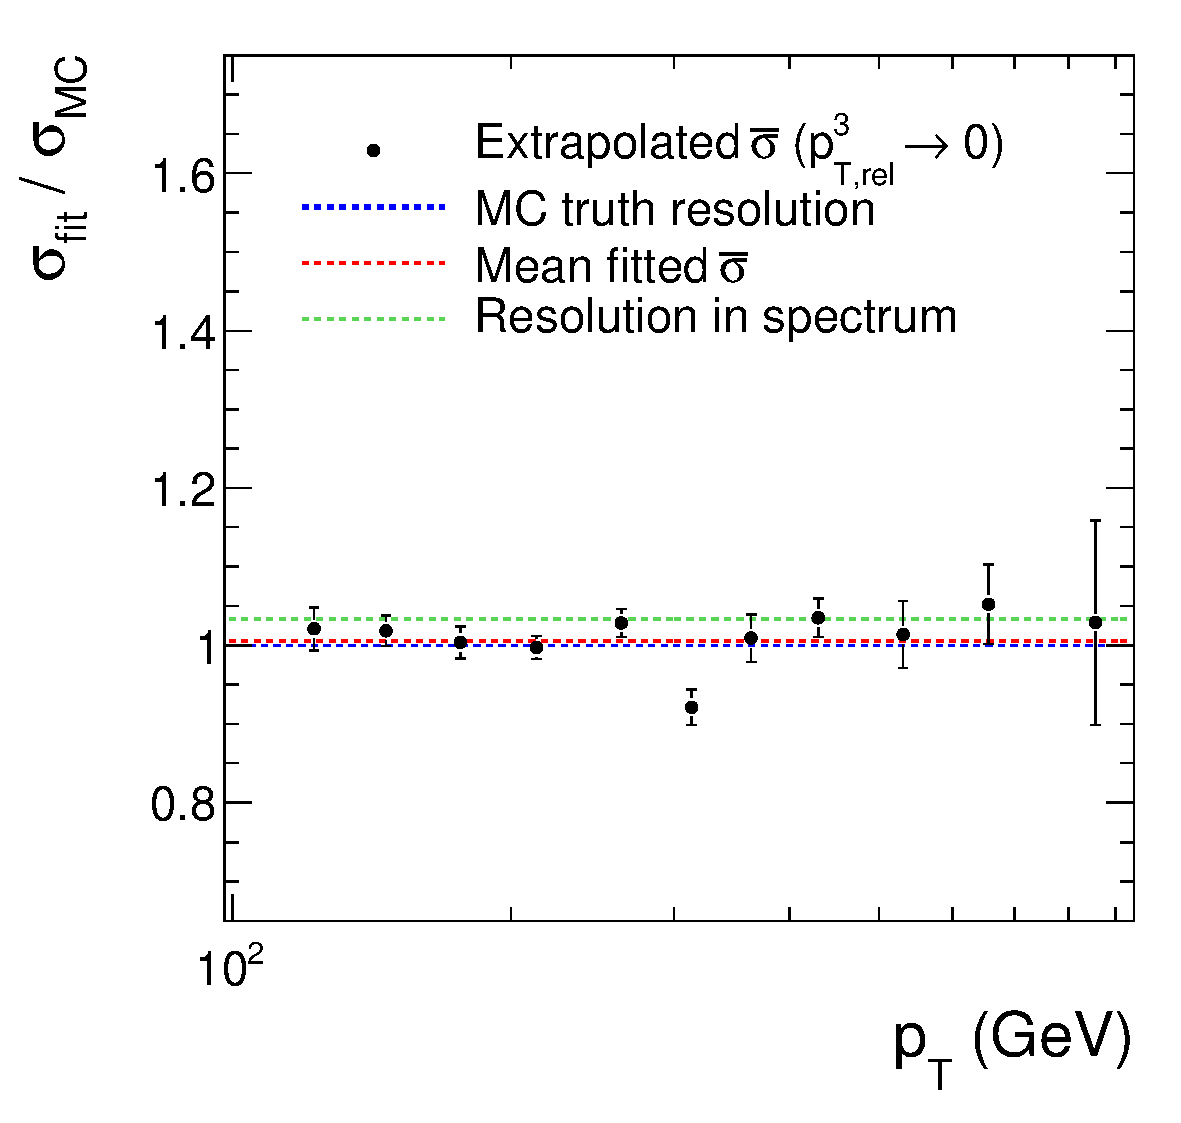
\includegraphics[width=0.3\textwidth]{figures/ResFit_Spring10QCDFlat_GaussUp30It1_Eta0_ExtrapolatedResolutionRatio} &
      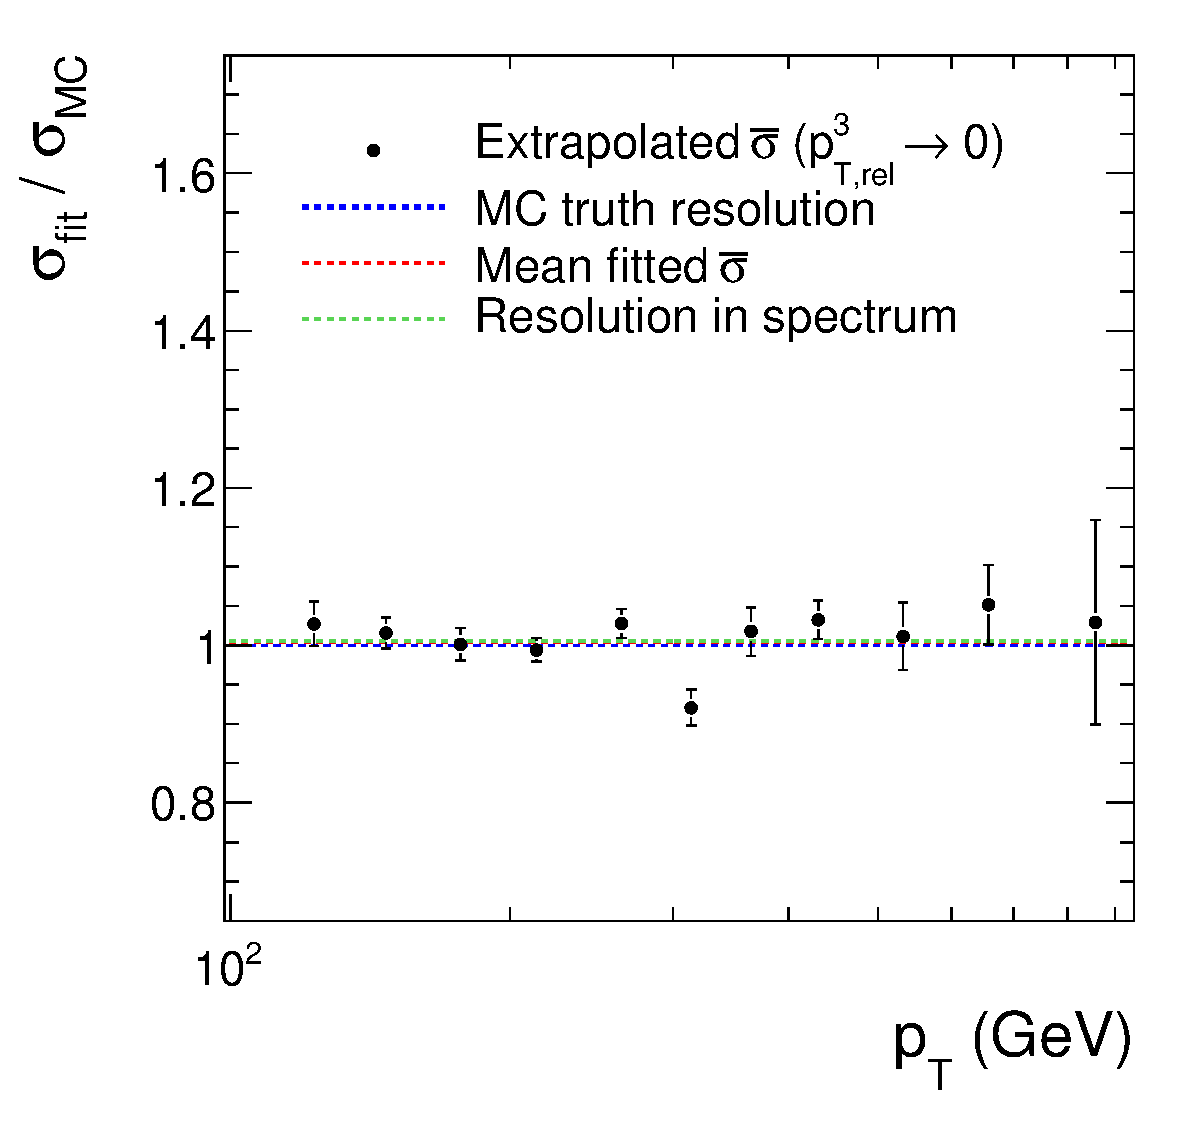
\includegraphics[width=0.3\textwidth]{figures/ResFit_Spring10QCDFlat_GaussUp30It2_Eta0_ExtrapolatedResolutionRatio}
    \end{tabular}
  \caption{The solid black markers show the measured Gaussian jet \pt resolutions in different \pt bins.
  The dashed green line is the assumed resolution to describe the selection bias during the fit.
  The dashed red line corresponds to the average measured resolution.
  Actually shown is the ratio to the Monte Carlo truth resolution in all cases.
  (\textit{Left}) The assumed resolution deviates by $30\%$ from the truth, the measured resolution by only $3.3\%$.
  (\textit{Centre}), (\textit{right}) The measured resolution from the previous iteration is taken as assumed resolution during the fit.
  The plots demonstrate the stability of an iterative procedure.}
  \label{fig:ResFig:QCD:Extrapolation:Gauss:Iterations}
\end{figure}

A description of the selection bias has been incorporated into the dijet probability density by assuming a jet \pt response $r_{0}(x|\pttrue)$ (Section~\ref{sec:ResFit:Method:Biases}).
In order to evaluate the influence of $r_{0}$ on the measured resolution, the fit has been performed with $r_{0}$ varied by $+30\%$ i.e. $\sigma_{0}\rightarrow 1.3\sigma_{0}$ (Fig.~\ref{fig:ResFig:QCD:Extrapolation:Gauss:Iterations}~\textit{left}).
The measured resolution deviates by $+(3.3 \pm 0.7)\%$ on average, demonstrating the weak influence of $r_{0}$ on the result.
A second and a third measurement have been performed, each time with the result of the previous as input for $r_{0}$, leading to decreasing average deviations (comp. Fig~\ref{fig:ResFig:QCD:Extrapolation:Gauss:Iterations} \textit{centre}, \textit{right}).
Hence, an iterative procedure is applicable. 



\subsubsection{Measurement of the full response function}\label{sec:ResFit:QCDMC:CrystalBall}

% $Id: Note_ResFit_Todo.tex,v 1.3 2010/07/08 14:32:36 mschrode Exp $


\section{Todo\ldots}

\subsection{Analysis}
\begin{itemize}
\item Extrapolation of (correlated!) Crystal Ball parameters ok?
\item Difference $\pt^{\text{parton}} \leftrightarrow \pt^{\text{particleJet}}$
\end{itemize}


\subsection{Note}

\subsubsection{Content}
\begin{itemize}
\item Advantage of an unbinned fit: works for less events
  \begin{itemize}
  \item Higher \pt reach
  \item Sensitivity to tails (paragraph on why tails are important)
  \end{itemize}
\item Advantage of a \pt dependent $\sigma$
  \begin{itemize}
  \item Fitted $\sigma$ also in spectrum (resolutin bias description)
  \end{itemize}
\item Motivate parametrisation of resolution in \pt
\item Closure plots
  \begin{itemize}
  \item MC truth response distributions
  \item Dijet asymmetry distributions
  \item Parameter scan plots
  \end{itemize}
\end{itemize}

\subsubsection{Style}
\begin{itemize}
\item Define consequently all quantities, in particular: $\pt^{\text{particle}}$ is particle jet \pt
\end{itemize}



% ----- This should all go to external files ------------
% \section{Determination of a Gaussian resolution}
% \subsection{Conceptual studies using a simple simulation}
% The method presented in the previous section has been studied using a
% simple simulation.

% \begin{figure}[ht]
%   \begin{center}
%      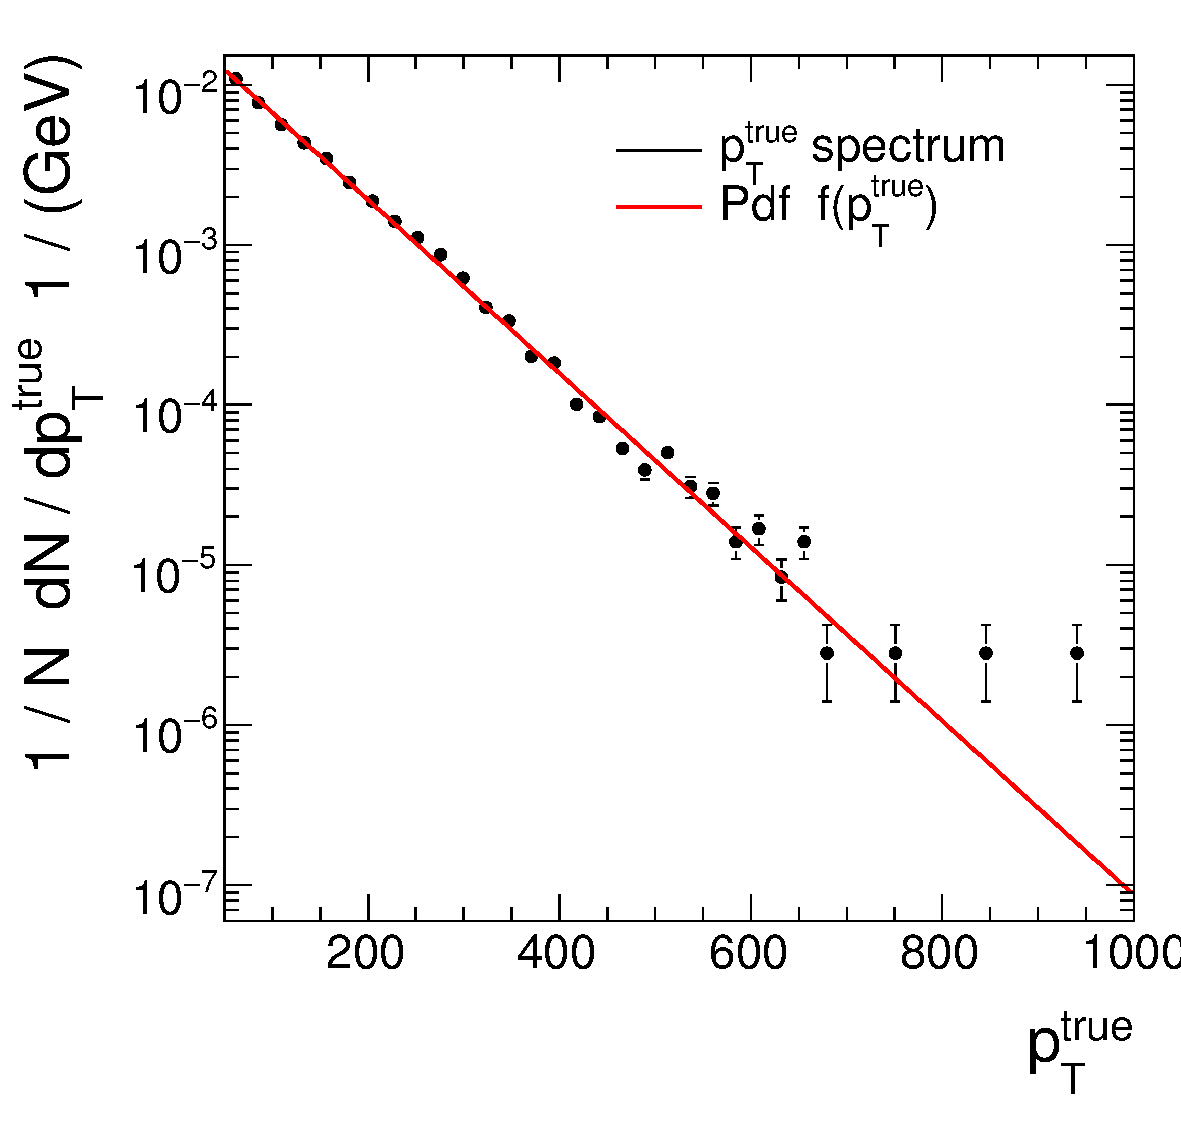
\includegraphics[width=0.45\textwidth]{figures/resFit_ToyMC_PtGenCuts_SpectrumLog}
%    \end{center}
%    \caption{Simple simulation of a sample of ideal dijet events.
%      Generated \pttrue spectrum (histogram) and the underlying pdf (solid line).}
%    \label{fig:resFit:toyMC:ptGenCuts:spectrum}
% \end{figure}

% \begin{figure}[ht]
%   \begin{center}
%     \subfigure[]{
%       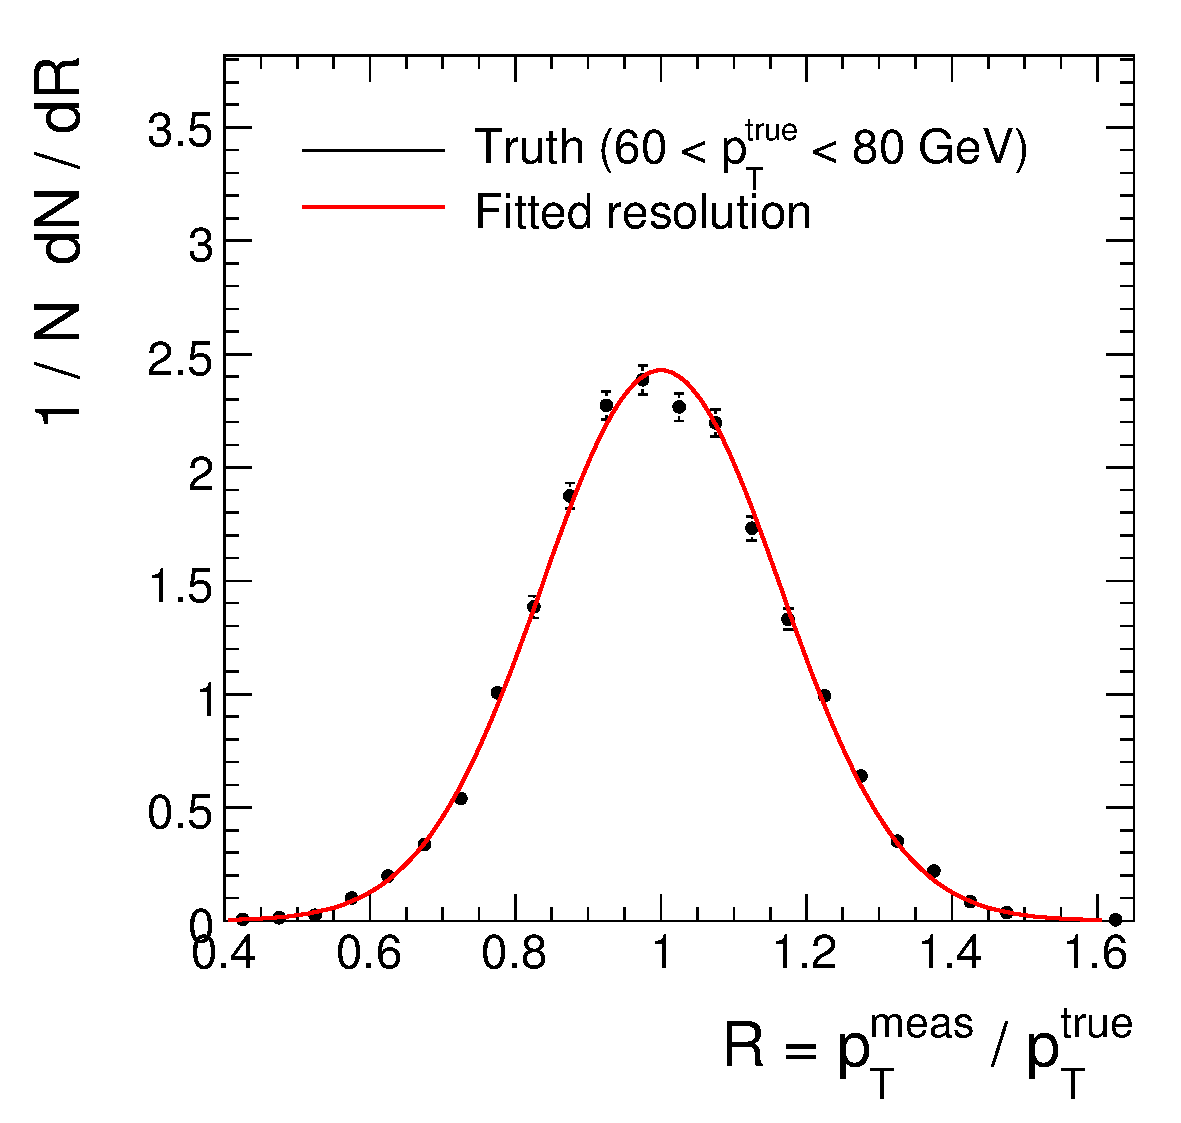
\includegraphics[width=0.45\textwidth]{figures/resFit_ToyMC_PtGenCuts_ResolutionBin1}
%    } \subfigure[]{
%       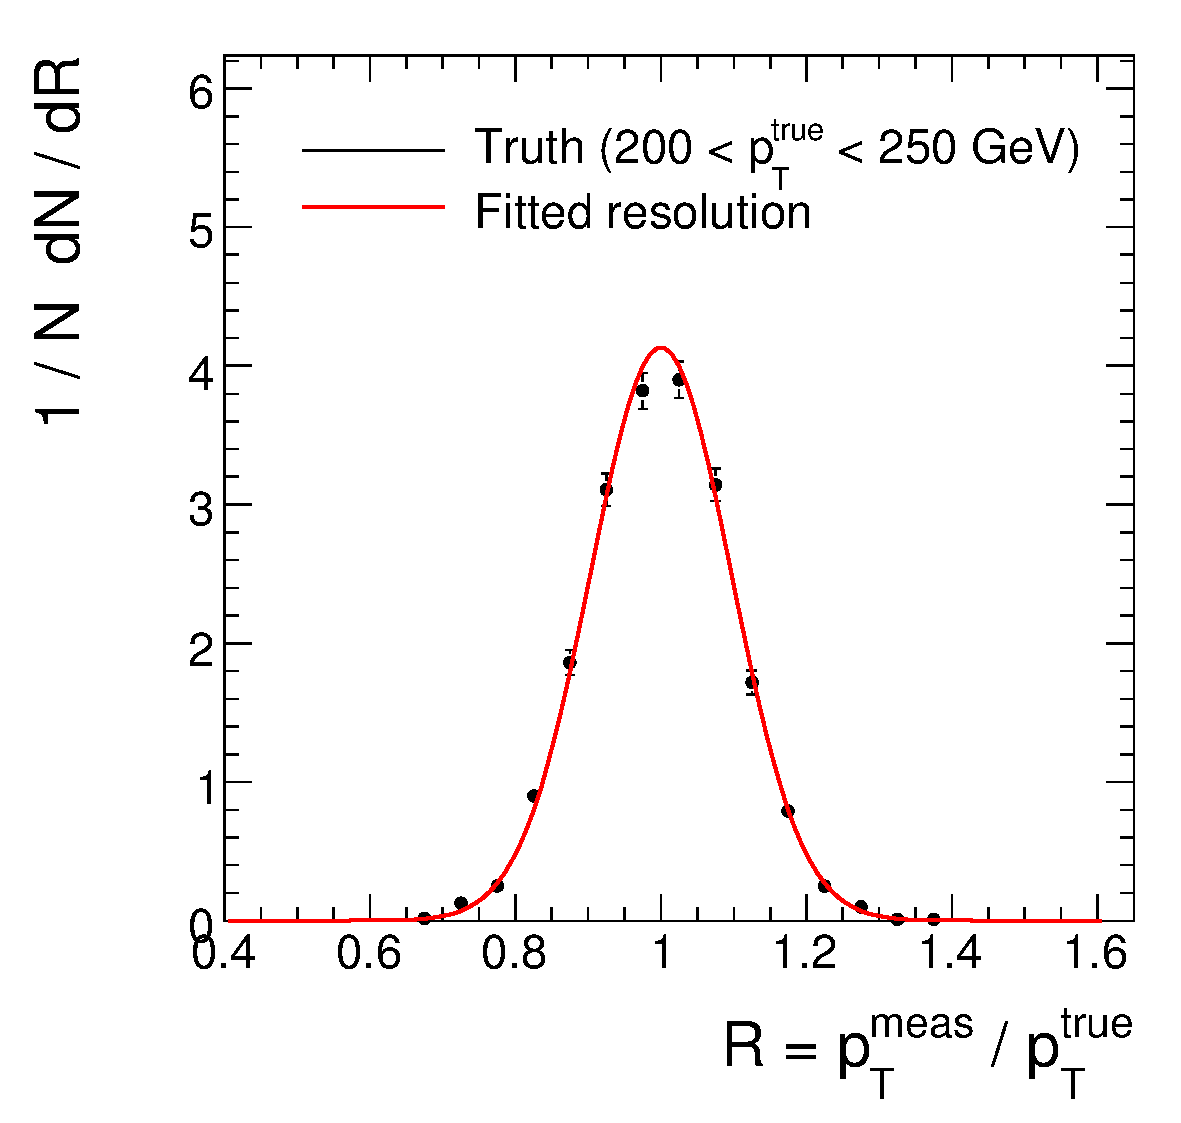
\includegraphics[width=0.45\textwidth]{figures/resFit_ToyMC_PtGenCuts_ResolutionBin7}
%    }
%   \end{center}
%   \caption{Simple simulation of a sample of ideal dijet events.
%     Generated true resolution \mbox{$\ptmeas / \pttrue$} (histogram) and the resolution (solid line) from the maximum likelihood fit in two different \pttrue bins.
%     Note, here ``fit'' does not refer to a fit to the shown histogram but the maximisation of the likelihood~\eqref{eq:resFit:likelihood}.
%   }
%   \label{fig:resFit:toyMC:ptGenCuts:reso}
% \end{figure}

% A sample of 30000 ideal dijet events has been generated with an
% exponentially falling spectrum
% \begin{equation}
%   \label{eq:resFit:toyMCSpec}
%   f\left(\pttrue\right) \propto \exp\left(-\pttrue / \tau\right),
%   \qquad \tau = 80.
% \end{equation}
% ranging from \mbox{$50 < \pttrue < 1000\gev$} (comp. Fig.~\ref{fig:resFit:toyMC:ptGenCuts:spectrum}).
% Two independent measurements of the jet \pt have been simulated
% from a Gaussian resolution
% \begin{equation}
%   \label{eq:resFit:toyMCRes}
%   f_{\vec{b}}\left(\ptmeas|\pttrue\right) = 
%   \frac{1}{\sqrt{2\pi}\sigma}\exp\left[-\frac{1}{2}\left(\frac{\ptmeas - \pttrue}{\sigma}\right)^{2}\right]
% \end{equation}
% (Here and in the following the jet index $i$ has been omitted.)
% The width $\sigma$ has been parameterised as a function of \pttrue and
% the parameters $b_{i}$, \mbox{$i\in\left\{0,2\right\}$}, as
% \begin{equation}
%   \label{eq:resFit:toyMCSigma}
%   \sigma = b_{0}\gev
%   \oplus b_{1}\,\sqrt{\pt\gev}\oplus b_{2}\pt.
% \end{equation}
% The parameter values of the parameters $\vec{b}$ are listed in
% Tab.~\ref{tab:resFit:toyMC:ptGenCuts:fitResult}.
% An example of the simulated resolution is shown in Fig. ~\ref{fig:resFit:toyMC:ptGenCuts:reso}.

% \begin{table}[ht]
%   \centering
%   \begin{tabular}[ht]{lccc}
%     \hline \hline
%     $b_{i}$ & $0$ & $1$ & $2$ \\
%     \hline
%     True value & $4$           & $1.2$           & $0.05$ \\
%     Fit result & $4.5 \pm 0.7$ & $1.18 \pm 0.05$ & $0.051 \pm 0.004$ \\
%     \hline \hline
%   \end{tabular}
%   \caption{Parameter values of the width $\sigma(\pt)$ of the Gaussian
%     resolution. Listed are the true values used for the generation and
%     the fitted values. The uncertainties assigned to the fitted values
%     are the statistical uncertainties from the fit. The parameter
%     correlations are shown in Fig.~\ref{fig:resFit:toyMC:ptGenCuts:parCorr}.}
%   \label{tab:resFit:toyMC:ptGenCuts:fitResult}
% \end{table}

% The jet energy resolution of this dijet sample is to be fitted using the method described above.
% In order to evaluate the dijet pdf~\eqref{eq:resFit:dijetPdf}, the spectrum $f(\pttrue)$ has to be known and the resolution $f_{\vec{b}}(\ptmeasi{i}|\pttrue)$ has to be parameterised appropriately.
% The spectrum is taken directly from the simulation~\eqref{eq:resFit:toyMCSpec}.
% If the same strategy is applied in data, influences of the uncertainty on the simulated spectrum on the fitted resolution have to be considered.
% These are small as shown in Section~\ref{sec:resFit:toyMC:uncert}.
% The resolution is parameterised with a Gaussian, where the width $\sigma$ depends on \pttrue and the parameters $\vec{b}$ as in~\eqref{eq:resFit:toyMCSigma}.
% The dijet pdf is normalised to the \pttrue range of the simulation i.e. $t_{0} = 50\gev$ and $t_{1} = 1000\gev$.
% This setup corresponds to cuts on \pttrue; a more data driven approach is discussed in Section~\ref{sec:resFit:dataDrivenExt}.

% \begin{figure}[ht]
%   \centering
%   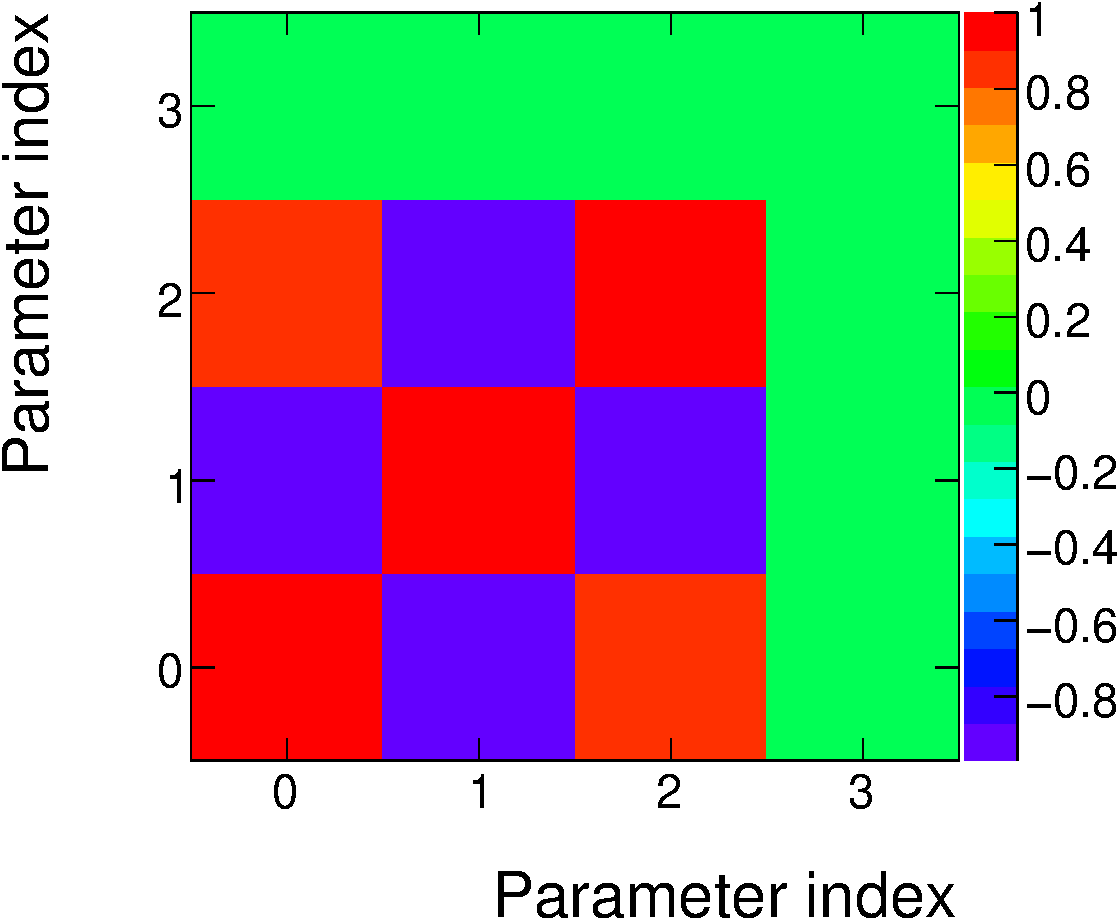
\includegraphics[width=0.45\textwidth]{figures/resFit_ToyMC_PtGenCuts_Correlations}
%   \caption{Correlation coefficients of the fitted parameter values
%     $\vec{b}$ of the width $\sigma$ of the Gaussian
%     resolution. Parameter $3$ corresponds to the slope $\tau$ of the
%     spectrum, which is fixed during the fit, and is to be ignored.}
%   \label{fig:resFit:toyMC:ptGenCuts:parCorr}
% \end{figure}

% The fitted parameter values $\vec{b}$ are listed in Tab.~\ref{tab:resFit:toyMC:ptGenCuts:fitResult}.
% They agree with the true values within the statistical uncertainties.

% The parameters are strongly (anti-) correlated (comp. Fig.~\ref{fig:resFit:toyMC:ptGenCuts:parCorr}).
% In the present \pttrue interval from \mbox{$t_{0} = 50\gev$} to \mbox{$t_{1} = 1000\gev$}, the used parameterisation of the Gaussian width $\sigma$ is over-determined.
% The $b_{0}$ term in~\eqref{eq:resFit:toyMCSigma} is most important at very low \pt while the $b_{2}$ term dominats at very large \pt.
% Hence, omitting either the terms with $b_{0}$ and $b_{2}$ or the term with $b_{1}$ in~\eqref{eq:resFit:toyMCSigma} would have been sufficient to describe the measured events.

% \begin{figure}[ht]
%   \begin{center}
%     \subfigure[]{
%       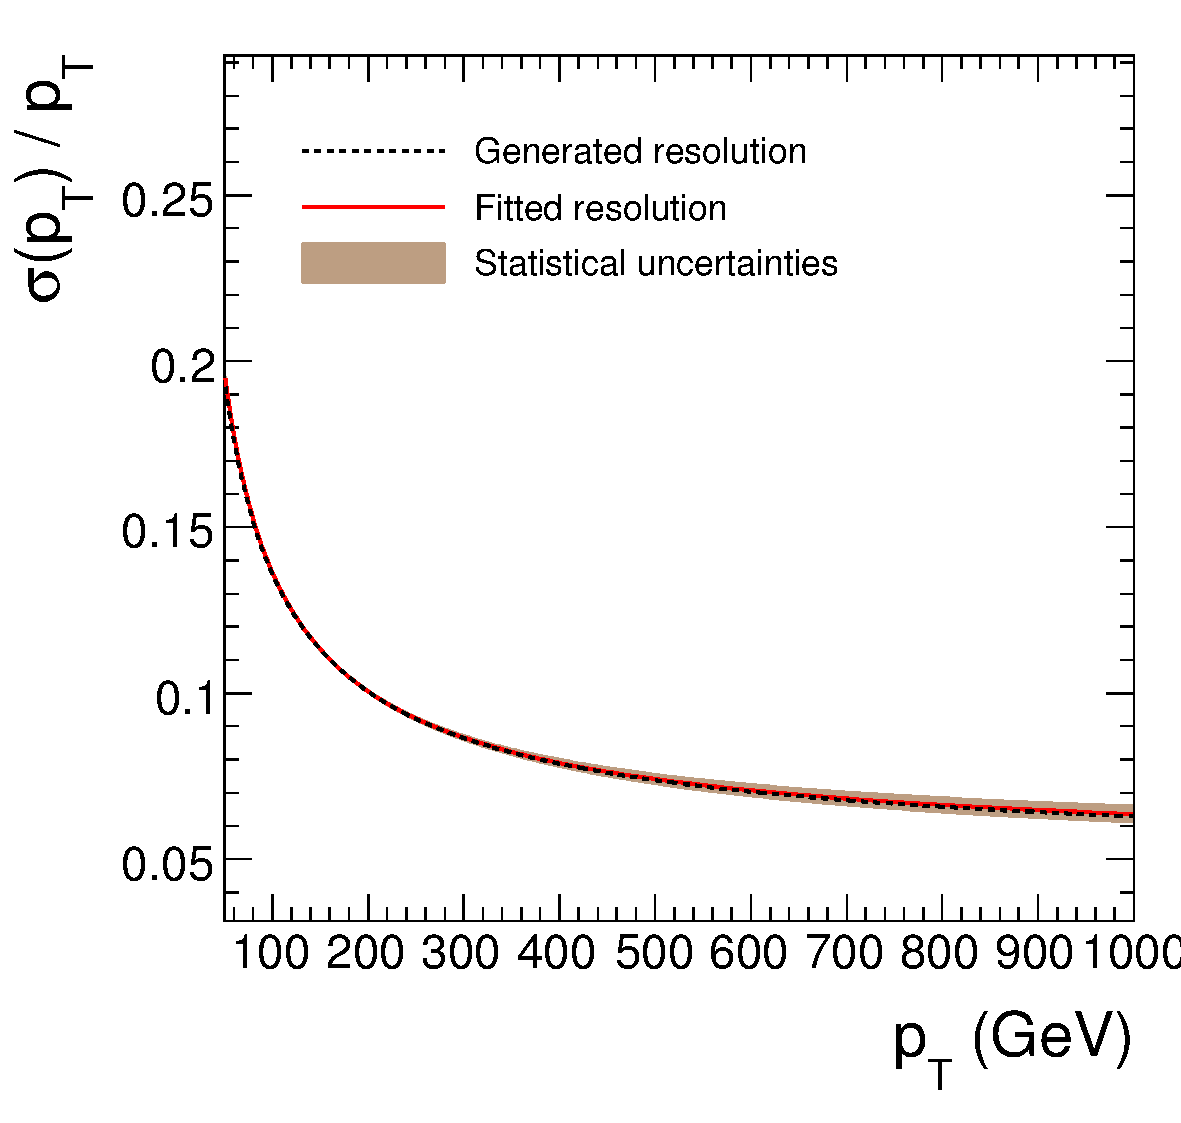
\includegraphics[width=0.45\textwidth]{figures/resFit_ToyMC_PtGenCuts_Sigma}
%   } \subfigure[]{
%       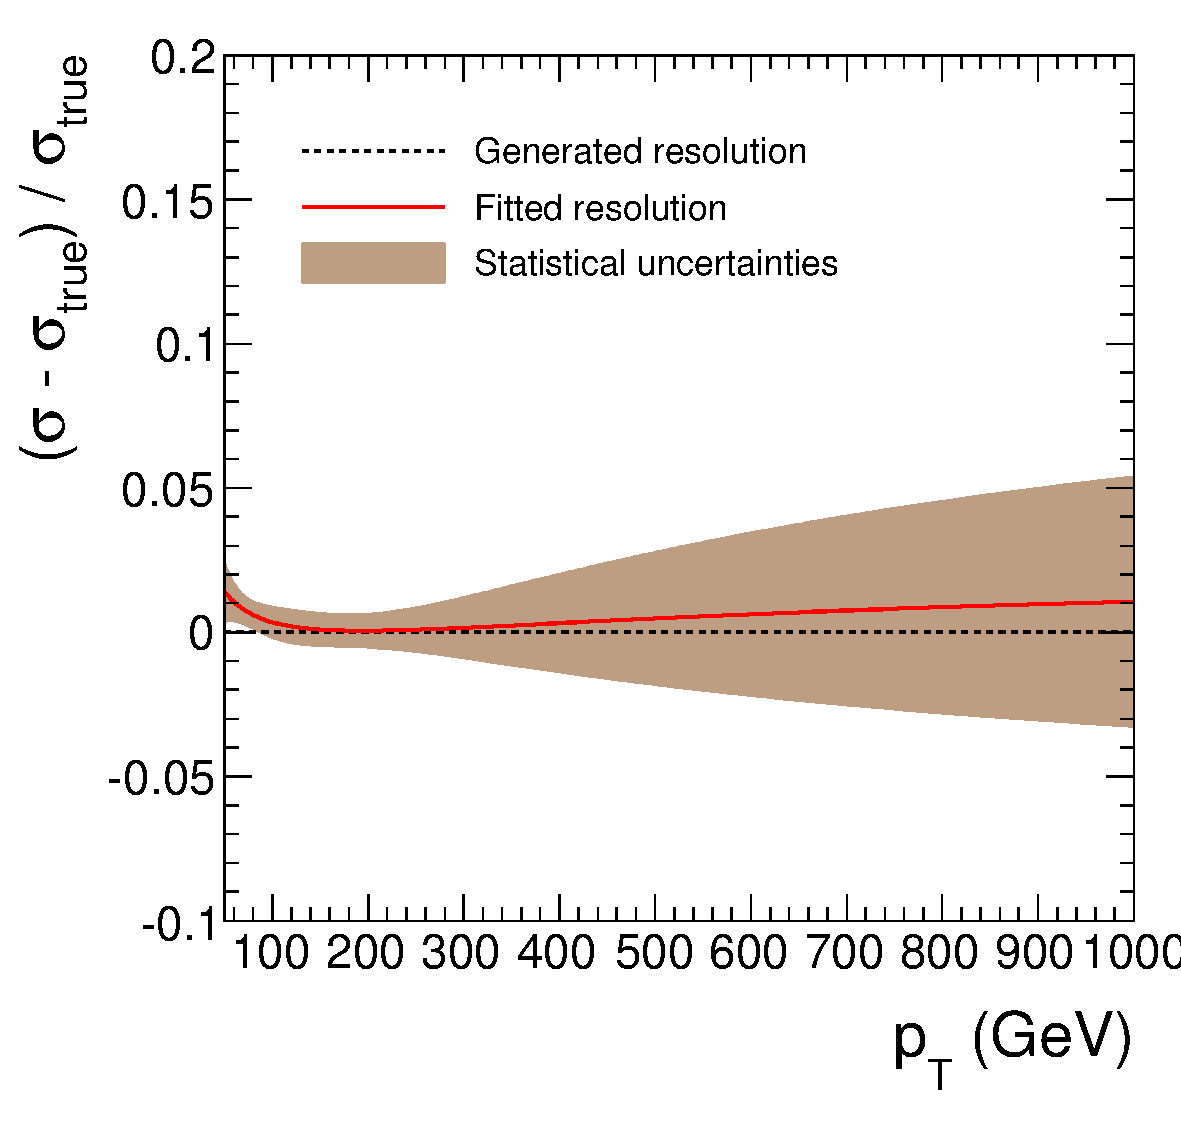
\includegraphics[width=0.45\textwidth]{figures/resFit_ToyMC_PtGenCuts_SigmaRelDifference}
%   }
%   \end{center}
%   \caption{(a) Relative Gaussian width $\sigma(\pt)/\pt$ evaluated with the fitted
%     parameter values (solid line) in comparison to the generated width
%     (dashed line).  (b) shows
%     the relative difference of the two curves. The shaded area represents the propagated statistical
%     uncertainty on the fitted parameter values, taking into account the
%     parameter correlations.}
%   \label{fig:resFit:toyMC:ptGenCuts:sigma}
% \end{figure}

% The relative Gaussian width $\sigma(\pt)/\pt$ evaluated with the fitted
% parameter values is shown in Fig.~\ref{fig:resFit:toyMC:ptGenCuts:sigma}
% in comparison to the true width at generation.
% There is good agreement between the fitted and the true resolution
% within the statistical uncertainties.
% The uncertainties are about $1\%$ at low \pt rising to
% about $3\%$ at $\pt \approx 600\gev$ where there is sufficient statistics in
% the generated sample (comp. Fig~\ref{fig:resFit:toyMC:ptGenCuts:spectrum}).
% For larger \pt the uncertainties rise up to $4.5\%$.

% An example of the resulting resolution in comparison to the true
% resolution is shown in Fig.~\ref{fig:resFit:toyMC:ptGenCuts:reso} for
% one \pttrue bin.


% \subsection{Extension to a data driven event selection}\label{sec:resFit:dataDrivenExt}

% So far, events have been selected by cuts on the true jet \pt.
% In a more data driven approach the selection is to be applied to the measured jet \pt.
% Events are selected, if for one of the two jets
% \begin{equation*}
%   \ptmin < \ptmeas < \ptmax.
% \end{equation*}
% Each event is considered twice; once for a \pt cut on the first and once for a \pt cut on the second jet.
% In this way any bias in the selection arising e.g. from always selecting the first and thus the jet fluctuated upwards is avoided and the available statistics is doubled.
% Since the \pt of the other jet can fluctuate arbitrarily, sensitivity to the resolution and in particular the non-Gaussian tails is assured; this is not the case when cutting e.g. on \mbox{$\ptdijet = \frac{1}{2}(\pt^{1}+pt^{2})$}, the average dijet \pt, as demonstrated in Fig.~\ref{fig:resFit:ptBinning}.

% \begin{figure}[ht]
%   \centering
%   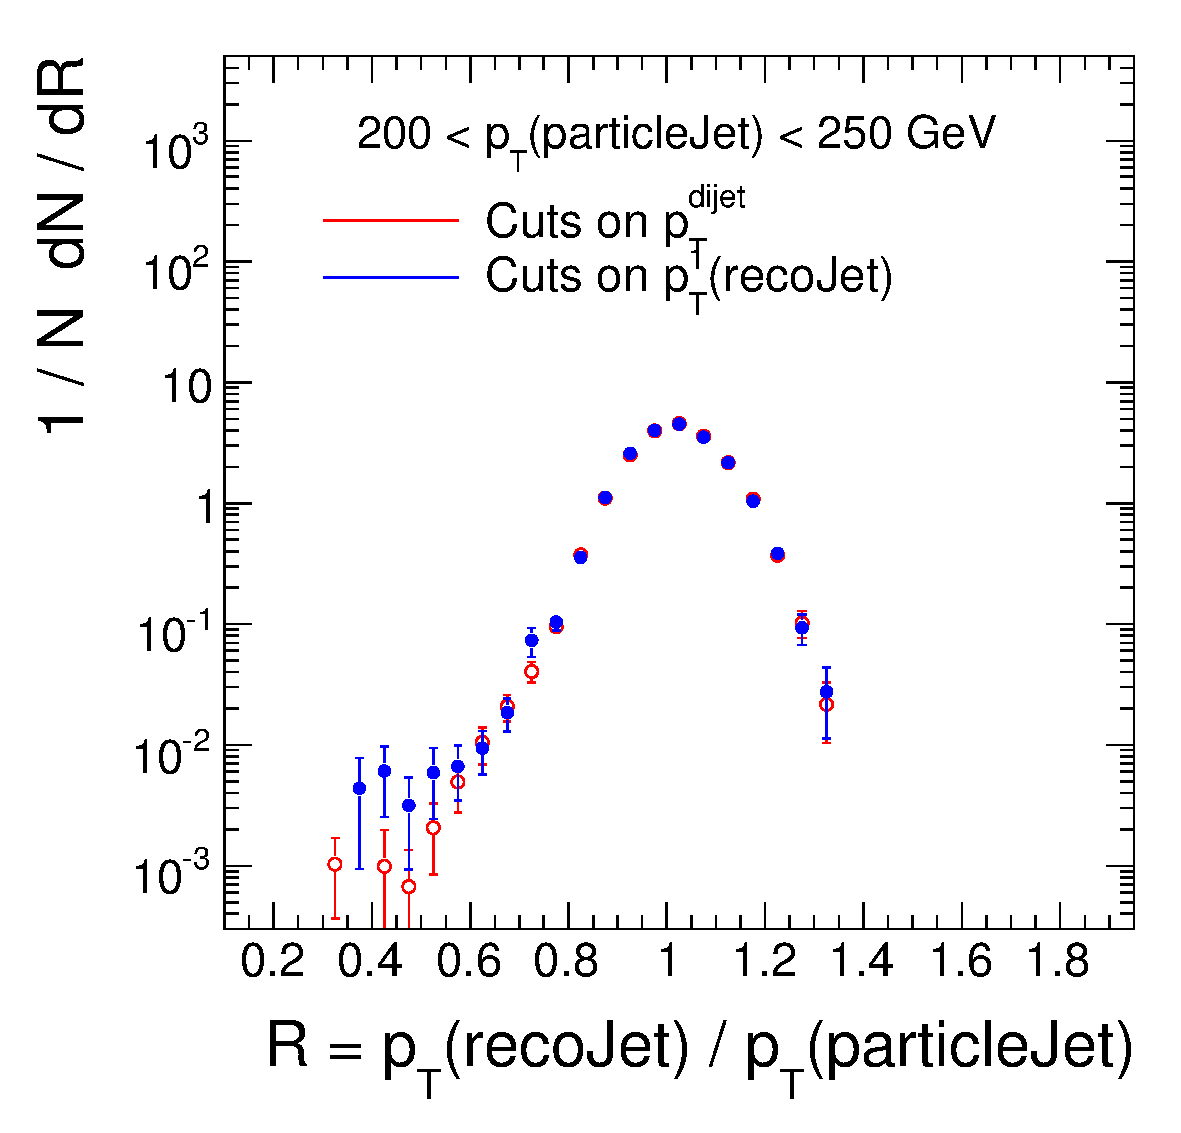
\includegraphics[width=0.45\textwidth]{figures/resFit_QCD_PtBinningComp}
%   \caption{Dependence of the true resolution on the definition of the quantity the cuts are applied to.
%     Cuts are applied either to \mbox{$\ptdijet = \frac{1}{2}(\pt^{1}+pt^{2})$} (open markers) or to the \pt of one of the jets while the other fluctuates arbitrarily (solid markers).
%     The non-Gaussian tails are surpressed when cutting on \ptdijet.}
%   \label{fig:resFit:ptBinning}
% \end{figure}

% Cutting on the measured \pt leads to migration effects at the edges of the selected \pt range due to the finite jet resolution.
% Considering the lower limit \ptmin, in an event with \mbox{$\pttrue < \ptmin$} the actually measured jet \pt might fluctuate upwards resulting in \mbox{$\ptmeas > \ptmin$} and thus false acceptance of the event.
% Similarly, events might be falsely rejected due to downward fluctuations.
% Since the dijet cross section is steeply falling with \pt, the described migration is asymmetric i.e. there is more upward than downward migration and more events are falsely accepted.
% (Analogue considerations hold true for the upper limit.)
% The described migration effects are demonstrated in Fig.~\ref{fig:resFit:toyMC:ptCuts:spectrum}.

% \begin{figure}[ht]
%   \begin{center}
%     \subfigure[]{
%       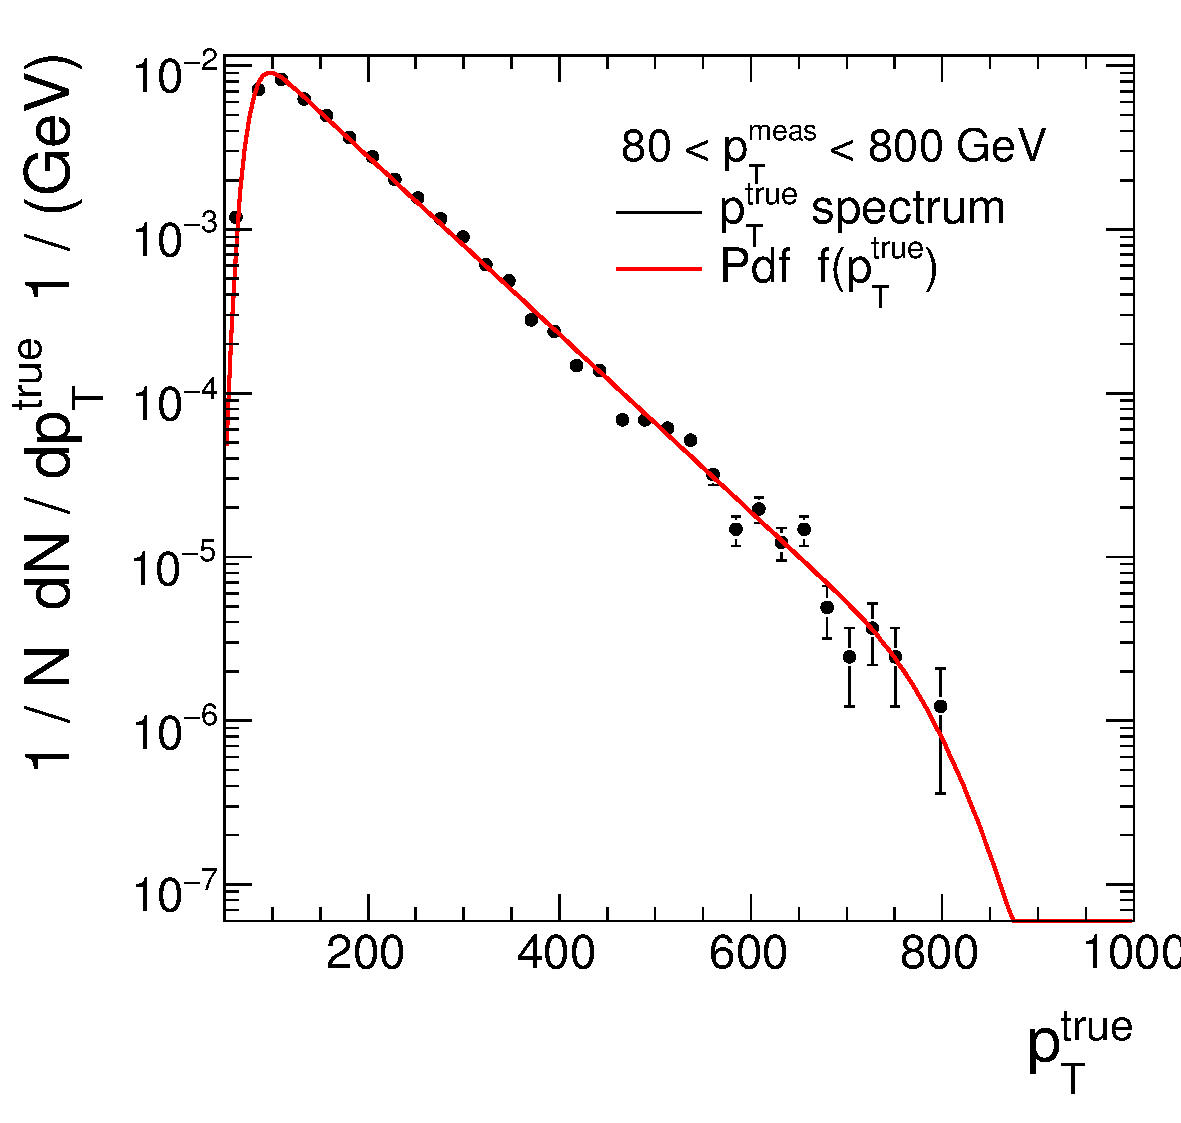
\includegraphics[width=0.45\textwidth]{figures/resFit_ToyMC_PtCuts_SpectrumLog}
%     } \subfigure[]{
%       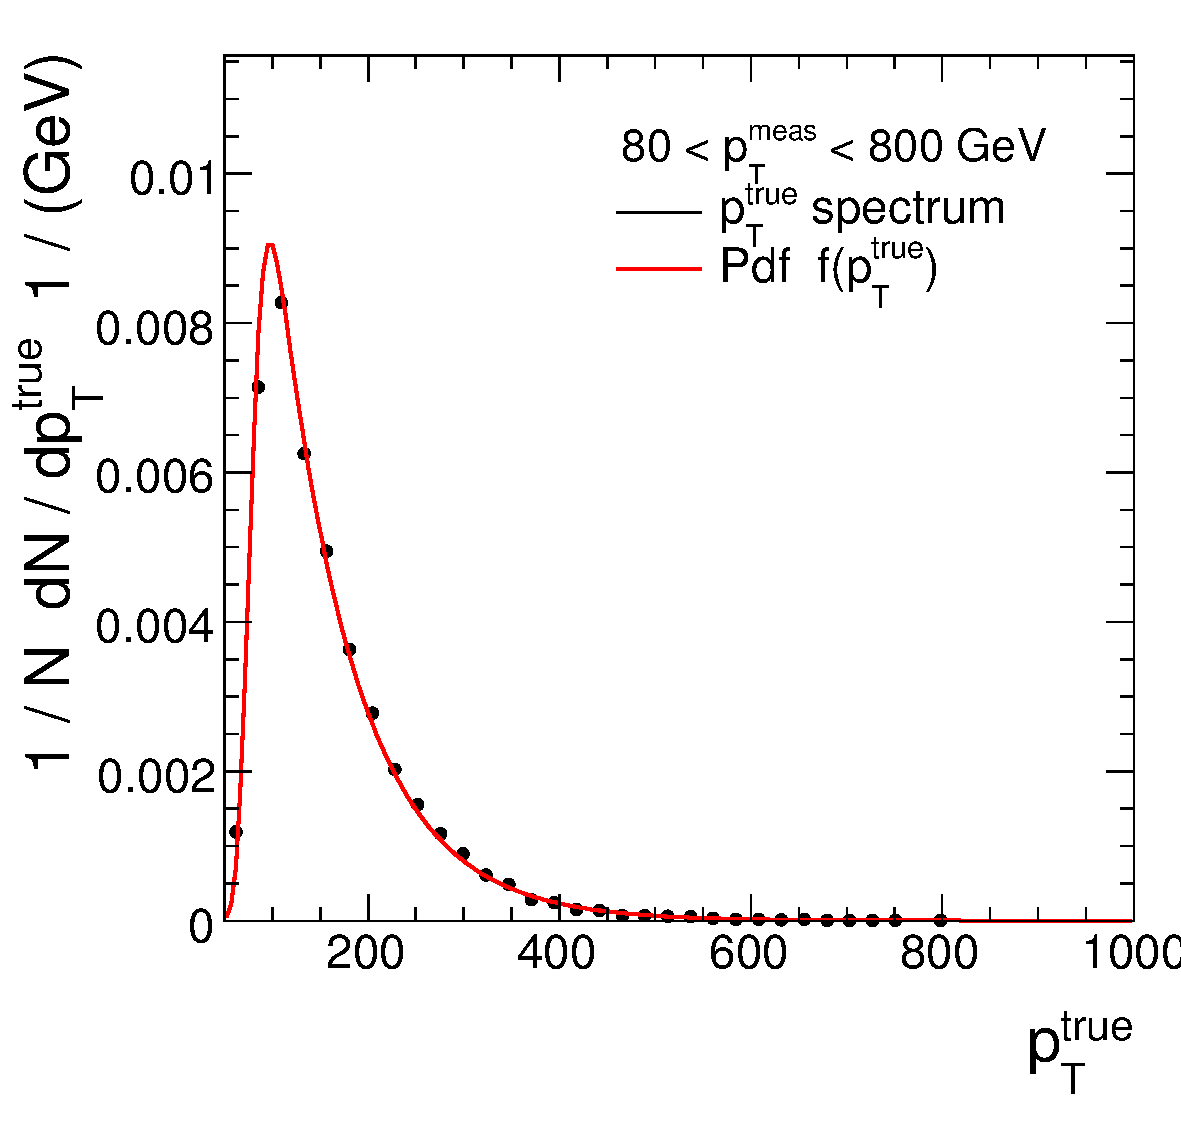
\includegraphics[width=0.45\textwidth]{figures/resFit_ToyMC_PtCuts_SpectrumLinear}
%     }
%   \end{center}
%   \caption{Simple simulation of a sample of ideal dijet
%     events. Generated \pttrue spectrum (histogram) and the underlying pdf (solid
%     line) after cuts on measured \pt. The spectrum is shown (a) in log
%     scale and (b) in linear scale.}
%   \label{fig:resFit:toyMC:ptCuts:spectrum}
% \end{figure}

% \begin{figure}[ht]
%   \begin{center}
%     \subfigure[]{
%       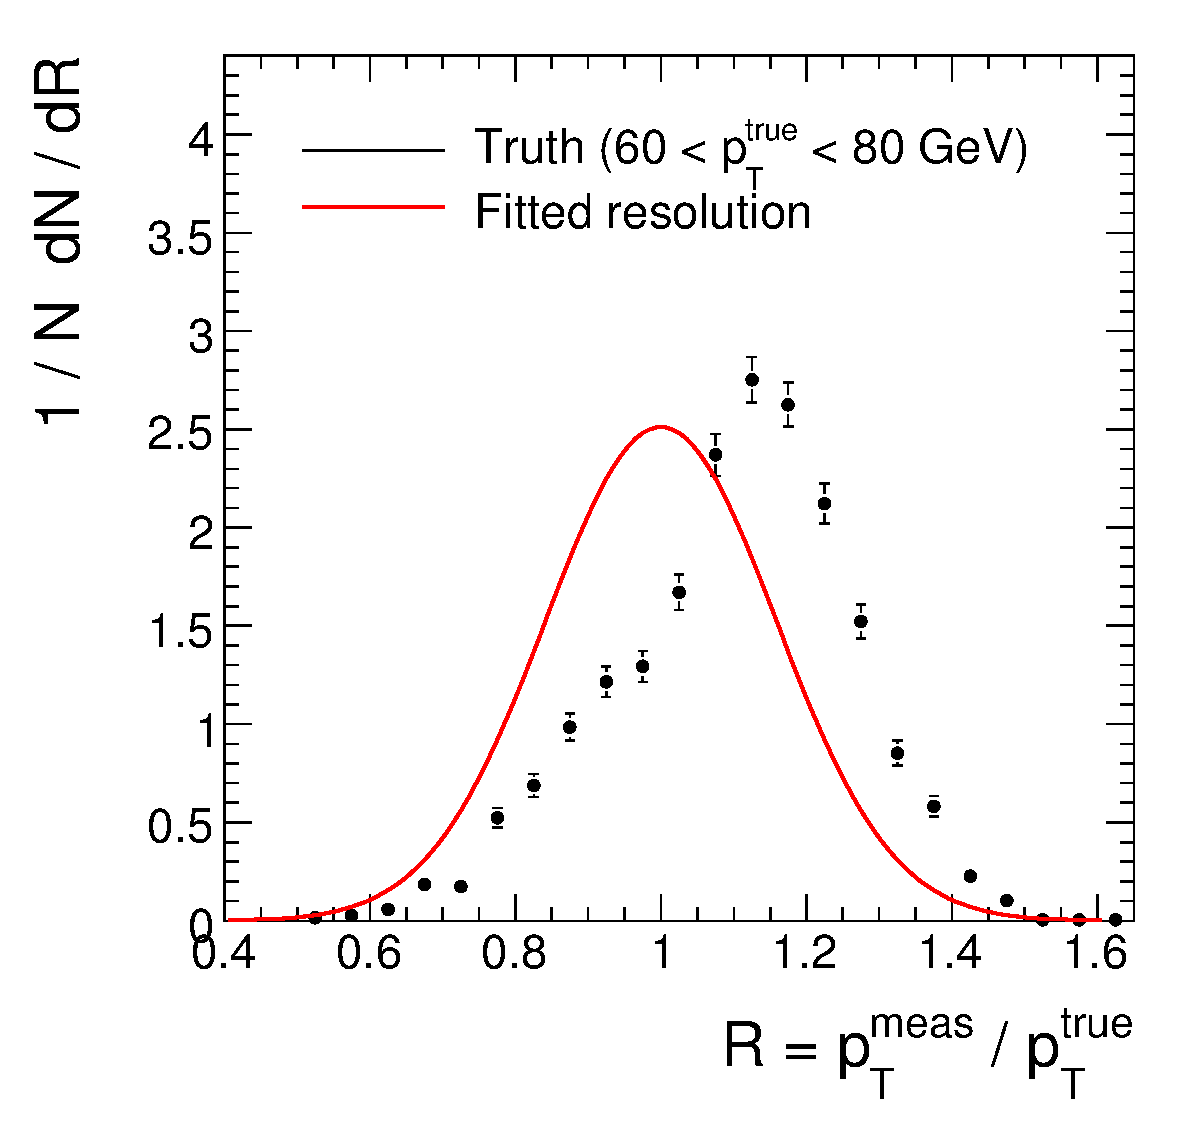
\includegraphics[width=0.45\textwidth]{figures/resFit_ToyMC_PtCuts_ResolutionBin1}
%    } \subfigure[]{
%       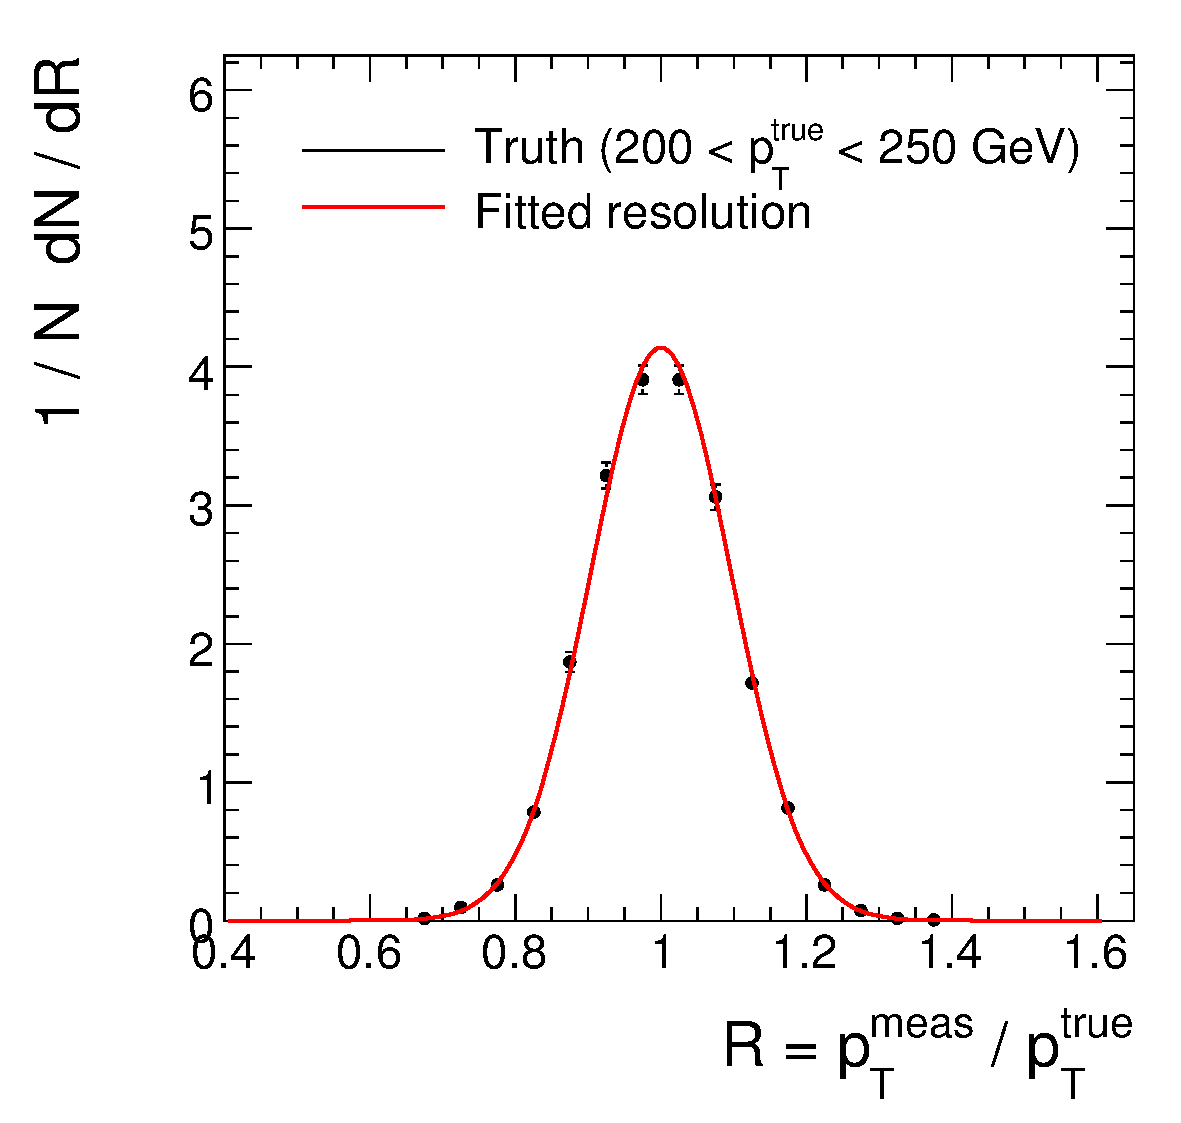
\includegraphics[width=0.45\textwidth]{figures/resFit_ToyMC_PtCuts_ResolutionBin7}
%    }
%   \end{center}
%   \caption{Simple simulation of a sample of ideal dijet
%     events. Generated true resolution \mbox{$\ptmeas / \pttrue$} (histogram) and the fitted
%     resolution (solid line) in two different \pttrue bins after cuts on measured \pt.
%     Note the migration effects in (a): the narrow peak at the right side is due to the jet that has been cut on and hence these are jets fluctuating upwards into the \pt bin.
%     The wider peak centered around one is due to the other jet that fluctuates unconstrained.
%     (There is more upward than downward fluctuation due to the falling spectrum.)
%   }
%   \label{fig:resFit:toyMC:ptCuts:reso}
% \end{figure}

% \begin{figure}[ht]
%   \begin{center}
%     \subfigure[]{
%       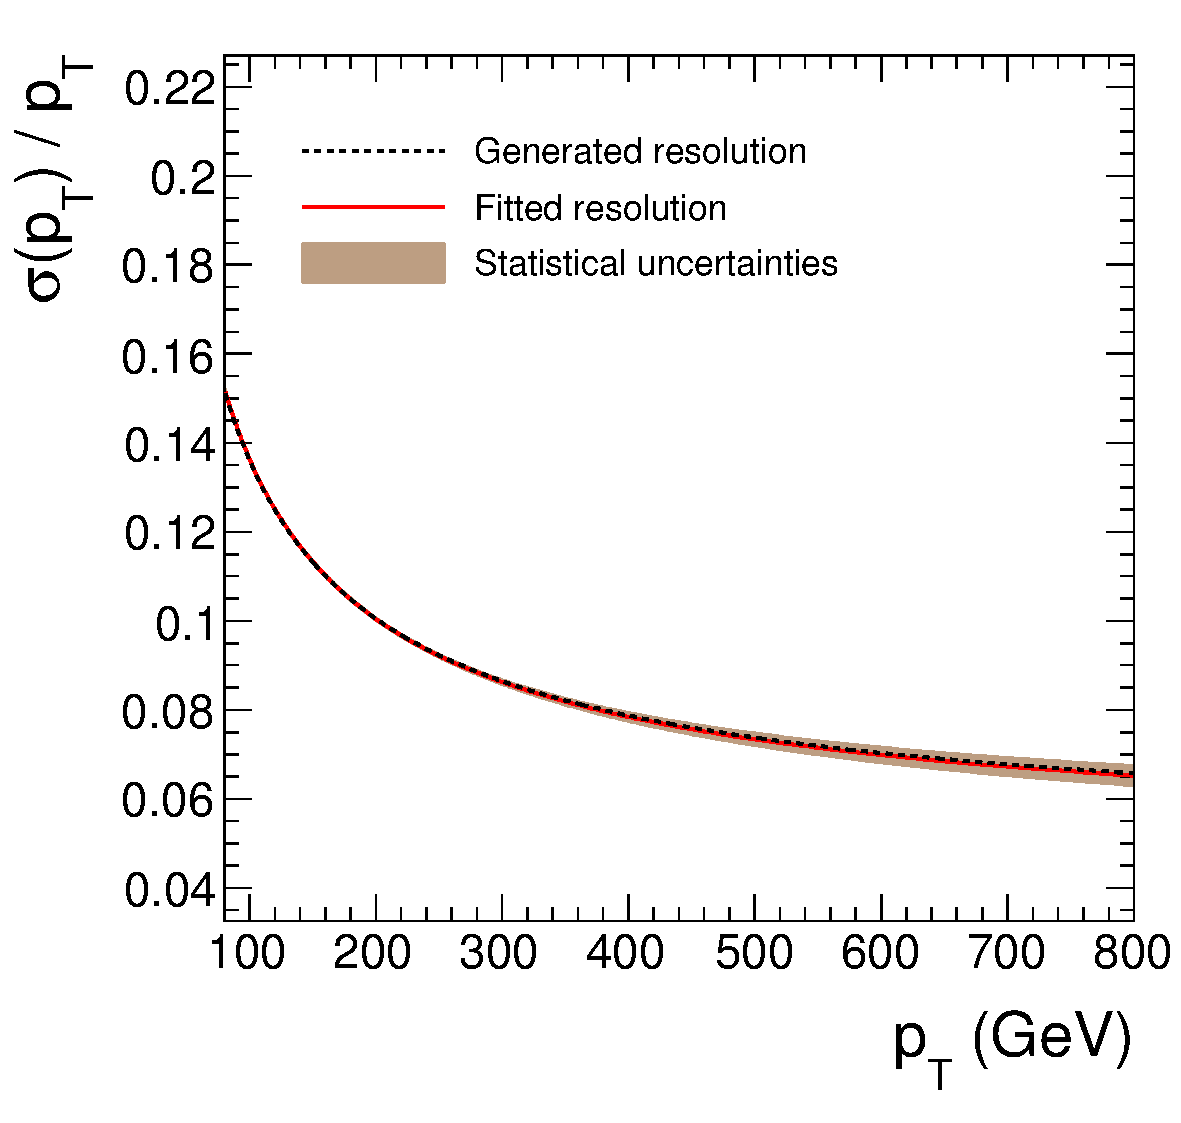
\includegraphics[width=0.45\textwidth]{figures/resFit_ToyMC_PtCuts_Sigma}
%   } \subfigure[]{
%       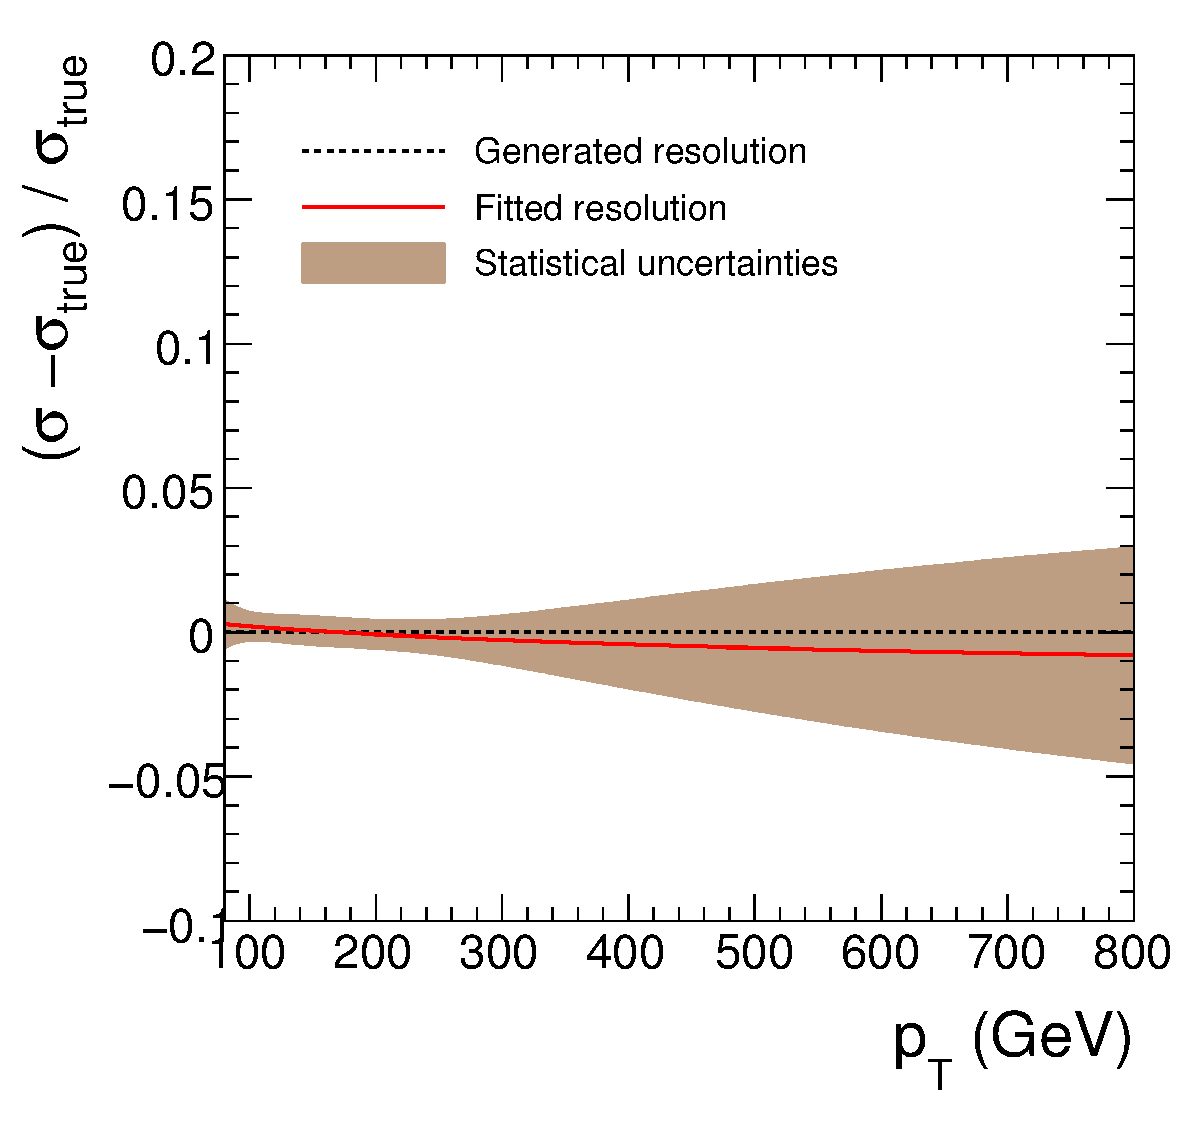
\includegraphics[width=0.45\textwidth]{figures/resFit_ToyMC_PtCuts_SigmaRelDifference}
%   }
%   \end{center}
%   \caption{(a) Relative Gaussian width $\sigma(\pt)/\pt$ evaluated with the fitted
%     parameter values (solid line) in comparison to the generated width
%     (dashed line). The fit has been performed after cuts on measured \pt. (b) shows
%     the relative difference of the two curves. The shaded area represents the propagated statistical
%     uncertainty on the fitted parameter values, taking into account the
%     parameter correlations.}
%   \label{fig:resFit:toyMC:ptCuts:sigma}
% \end{figure}

% The dijet pdf~\eqref{eq:resFit:dijetPdf} is adapted to include the cuts on the measured jet \pt.
% First, the allowed range of measured \pt is restricted for the jet the \pt cut is applied to.
% In the following, it is assumed that this is the first jet; the pdfs of measured jet \pt therefore become
% \begin{eqnarray*}
%   f_{\vec{b}}\left(\ptmeasi{1}|\pttrue\right) & = & 
%   \frac{1}{\mathcal{N}_{1}}\exp\left[-\frac{1}{2}\left(\frac{\ptmeasi{1}
%         - \pttrue}{\sigma}\right)^{2}\right]
%   \cdot\theta\left(\ptmeasi{1} - \ptmin\right)
%   \cdot\theta\left(\ptmax - \ptmeasi{1}\right) \\
%   f_{\vec{b}}\left(\ptmeasi{2}|\pttrue\right) & = & 
%   \frac{1}{\mathcal{N}_{2}}\exp\left[-\frac{1}{2}\left(\frac{\ptmeasi{2}
%         - \pttrue}{\sigma}\right)^{2}\right] \\
% \end{eqnarray*}
% with the normalisation constants
% \begin{eqnarray*}
%   \mathcal{N}_{1} & = &
%   \int^{\ptmax}_{\ptmin}\dif{\ptmeasi{1}}\,f_{\vec{b}}\left(\ptmeasi{1}|\pttrue\right)
%   = \sqrt{\frac{\pi}{2}}\sigma \left[ \text{erf}\left(\frac{\ptmax -
%         \pttrue}{\sqrt{2}\sigma}\right) - \text{erf}\left(\frac{\ptmin
%         - \pttrue}{\sqrt{2}\sigma}\right)\right] \\
%   \mathcal{N}_{2} & = &
%   \int^{\infty}_{0}\dif{\ptmeasi{2}}\,f_{\vec{b}}\left(\ptmeasi{2}|\pttrue\right)
%   = \sqrt{\frac{\pi}{2}}\sigma \left[ 1 +
%     \text{erf}\left(\frac{\pttrue}{\sqrt{2}\sigma}\right)\right]
%   \approx \sqrt{2\pi}\sigma.
% \end{eqnarray*}
% Second, the pdf of the true \pt is extended to incorporate the events
% migrating into the allowed \pt range by
% \begin{equation}
%   \label{eq:resFit:toyMC:ptCuts:extendedSpectrum}
%   \tilde{f}\left(\pttrue\right) = \frac{1}{\mathcal{N}_{\tilde{f}}}
%   f\left(\pttrue\right) \int^{\ptmax}_{\ptmin}\dif{x}\,f_{\text{MC}}\left(x|\pttrue\right)
% \end{equation}
% with the normalisation
% \begin{equation*}
%   \mathcal{N}_{\tilde{f}} = \int^{\infty}_{0}\dif{\pttrue}\,
%   f\left(\pttrue\right) \int^{\ptmax}_{\ptmin}\dif{x}\,f_{\text{MC}}\left(x|\pttrue\right).
% \end{equation*}
% Here, $f(\pttrue)$ denotes the underlying spectrum~\eqref{eq:resFit:toyMCSpec} and
% $f_{\text{MC}}(x|\pttrue)$ the pdf of measured \pt.
% $f_{\text{MC}}(x|\pttrue)$ in \eqref{eq:resFit:toyMC:ptCuts:extendedSpectrum} is taken from the
% simulation and the parameters are kept fixed during the maximisation.
% Thus usage of the simulation introduces a further uncertainty but they
% are small as in case of the underlying spectrum as shown below.
% The adapted dijet pdf then becomes
% \begin{equation}
%   \label{eq:resFit:toyMC:ptCuts:pdf}
%   f_{\vec{b}}\left(\ptmeasi{1},\ptmeasi{2}\right) = \int^{\infty}_{0}\dif{\pttrue}\,\tilde{f}\left(\pttrue\right)
%   \cdot f_{\vec{b}}\left(\ptmeasi{1}|\pttrue\right)
%   \cdot f_{\vec{b}}\left(\ptmeasi{2}|\pttrue\right),
% \end{equation}
% which is properly normalised to
% \begin{equation*}
%   1 = \int^{\ptmax}_{\ptmin}\dif{\ptmeasi{1}}\,\int^{\infty}_{0}\dif{\ptmeasi{2}}\, f_{\vec{b}}\left(\ptmeasi{1},\ptmeasi{2}\right).
% \end{equation*}

% \begin{table}[ht]
%   \centering
%   \begin{tabular}[ht]{lccc}
%     \hline \hline
%     $b_{i}$ & $0$ & $1$ & $2$ \\
%     \hline
%     True value & $4$           & $1.2$                   & $0.05$ \\
%     Fit result   & $4 \pm 1$ & $1.20 \pm 0.07$ & $0.049 \pm 0.005$ \\
%     \hline \hline
%   \end{tabular}
%   \caption{Parameter values of the width $\sigma(\pt)$ of the Gaussian
%     resolution. Listed are the true values used for the generation and
%     the fitted values. The fit has been performed after cuts on measured \pt.
%     The uncertainties assigned to the fitted values
%     are the statistical uncertainties from the fit; correlations are not shown.}
%   \label{tab:resFit:toyMC:ptCuts:fitResult}
% \end{table}

% Again the sample of ideal dijet events is used to test the discussed extension of the method.
% Cuts are placed on the measured \pt at \mbox{$\ptmin = 80\gev$} and \mbox{$\ptmax = 800\gev$} (comp. Fig.~\ref{fig:resFit:toyMC:ptCuts:spectrum}).
% The jet energy resolution of the selected dijet events is fitted using the modified pdf~\eqref{eq:resFit:toyMC:ptCuts:pdf}.
% Uncertainties due to uncertainties in the description of the spectrum are discussed in Section~\ref{sec:resFit:toyMC:uncert}.

% The fitted parameter values $\vec{b}$ of the Gaussian width $\sigma$ are listed in Tab.~\ref{tab:resFit:toyMC:ptCuts:fitResult}.
% They agree with the true values within the statistical uncertainties.
% As expected, they feature the same correlation pattern as in case of \pttrue cuts.

% The relative Gaussian width $\sigma(\pt)/\pt$ evaluated with the fitted parameter values is shown in Fig.~\ref{fig:resFit:toyMC:ptCuts:sigma} in comparison to the true width at generation.
% There is good agreement between the fitted and the true resolution within the statistical uncertainties.
% As before, the uncertainties are about $1\%$ at low \pt rising to about $3\%$ at $\pt \approx 600\gev$ and up to $4.5\%$ at very large \pt.
% An example of the resulting resolution in comparison to the true resolution is shown in Fig.~\ref{fig:resFit:toyMC:ptCuts:reso} for one \pttrue bin.

% It can be concluded therefore that the method is working also for a data driven event selection.



% \subsection{Estimation of systematic uncertainties}\label{sec:resFit:toyMC:uncert}

% The dijet pdf discussed above contains knowledge of the actual dijet spectrum and --- in case of cuts on measured jet \pt --- also of the resolution to describe the cut-off effects.
% When applying the method to data this information would be taken from a MC simulation.
% Test have been performed to evaluate the influence of uncertainties in the MC description on the fitted resolution.

% \begin{figure}[ht]
%   \centering
%   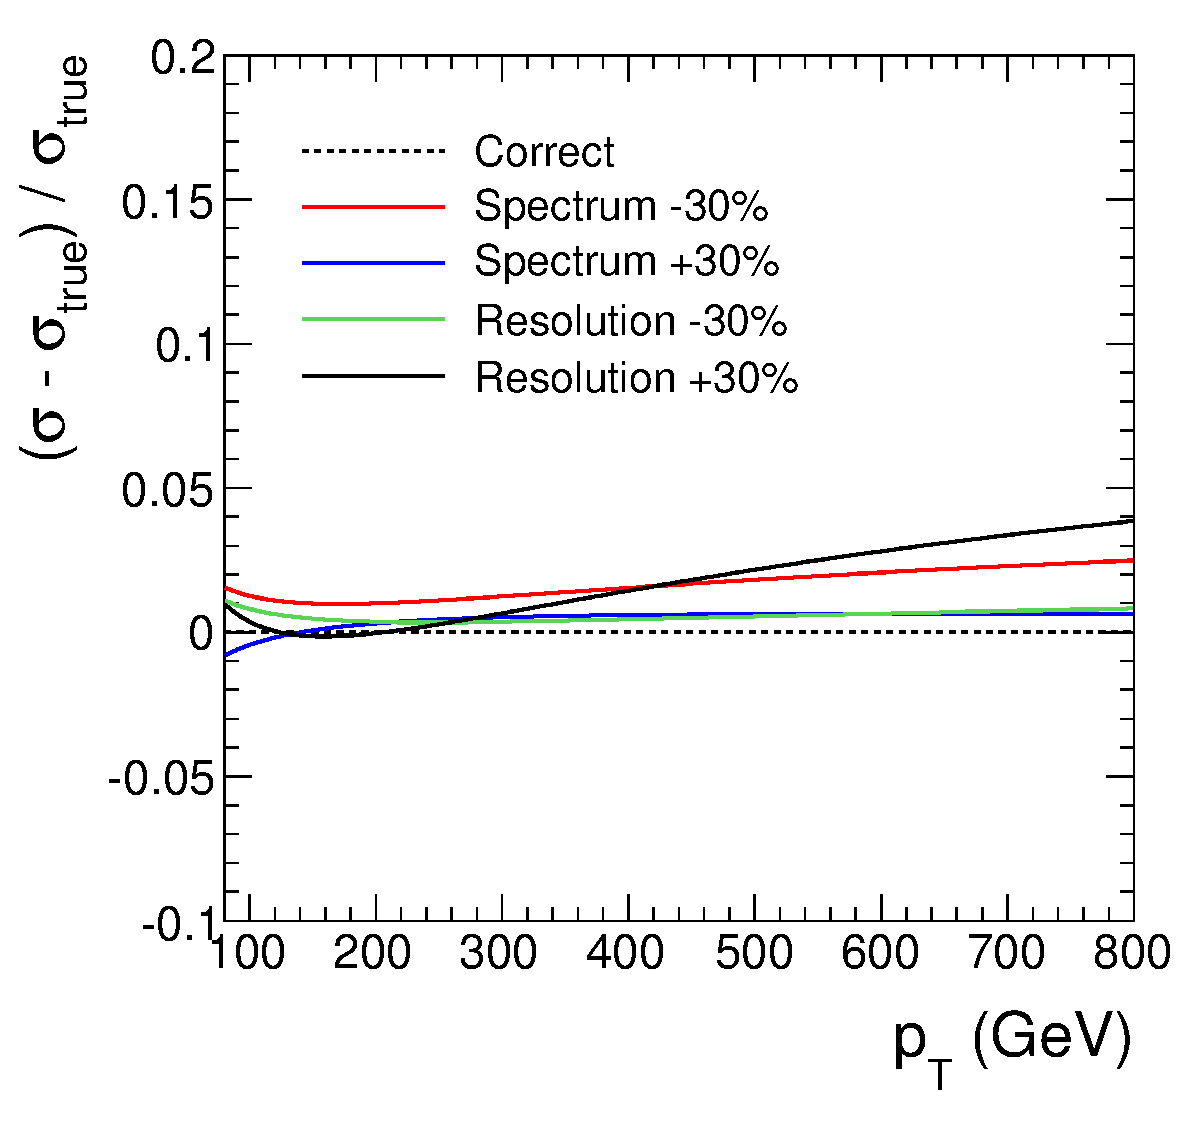
\includegraphics[width=0.45\textwidth]{figures/resFit_ToyMC_PtCuts_SigmaUncertainties}
%   \caption{Relative differences of the Gaussian widths $\sigma(\pt)$ evaluated with the fitted parameter values for different variations of the spectrum and the correct spectrum.
%     The variation has been applied to the slope parameter $\tau$ in \eqref{eq:resFit:toyMCSpec} (``Spectrum'') as well as all three parameters $b_{\text{MC},i}$ in \eqref{eq:resFit:toyMC:ptCuts:extendedSpectrum} (``Resolution'').}
%   \label{fig:resFit:toyMC:uncert:systUncertainties}
% \end{figure}

% \begin{table}[ht]
%   \centering
%   \begin{tabular}[ht]{lccc}
%     \hline \hline
%     $b_{i}$ & $0$ & $1$ & $2$ \\
%     \hline
%     True value         & $4$       & $1.2$           & $0.05$ \\
%     Correct            & $4 \pm 1$ & $1.20 \pm 0.07$ & $0.049 \pm 0.005$ \\
%     Spectrum $+30\%$   & $3 \pm 2$ & $1.22 \pm 0.07$ & $0.049 \pm 0.005$ \\
%     Spectrum $-30\%$   & $5 \pm 1$ & $1.19 \pm 0.08$ & $0.052 \pm 0.006$ \\
%     Resolution $+30\%$ & $5 \pm 1$ & $1.13 \pm 0.07$ & $0.054 \pm 0.004$ \\
%     Resolution $-30\%$ & $5 \pm 2$ & $1.19 \pm 0.08$ & $0.050 \pm 0.006$ \\
%     \hline \hline
%   \end{tabular}
%   \caption{Parameter values of the width $\sigma(\pt)$ of the Gaussian resolution.
%     Listed are the true values used for the generation and the fitted values for different variations of the spectrum.
%     The uncertainties assigned to the fitted values are the statistical uncertainties from the fit.}
%   \label{tab:resFit:toyMC:uncert:fitResult}
% \end{table}

% The fit has been repeated with the same setup as described in Section~\ref{sec:resFit:dataDrivenExt}.
% In order to evaluate the influence of the spectrum on the result the slope i.e. the parameter $\tau$ in \eqref{eq:resFit:toyMCSpec} has been varied by $\pm30\%$.
% Cut-off effects in the spectrum are described by the true resolution $f_{\text{MC}}(x|\pttrue)$ in \eqref{eq:resFit:toyMC:ptCuts:extendedSpectrum}.
% All three parameters $b_{\text{MC},i}$ of $f_{\text{MC}}(x|\pttrue)$ have been varied by $\pm30\%$ to evaluate uncertainties arising from the simulation.

% The fitted parameter values for each variation are listed in Tab.~\ref{tab:resFit:toyMC:uncert:fitResult} in comparion to the values obtained when using the correct spectrum.
% The relative differences of the Gaussian widths $\sigma$ calculated with these fitted parameter values to the $\sigma$ using the correct spectrum are presented in Fig.~\ref{fig:resFit:toyMC:uncert:systUncertainties} as a function of \pt for the different variations; they are below $4\%$.
% A varied spectrum predominantly results in a larger resolution.



% \subsection{Application to a realistic QCD simulation}\label{sec:resFit:qcdSelection}
% The method has then been applied to QCD events with 7\tev center of
% mass energy which were generated with PYTHIA and went through a full
% GEANT4 based CMS detector simulation\footnote{The used dataset is
%   \texttt{/QCDFlat\_Pt15to3000/Summer09-MC\_31X\_V9\_7TeV-v1/GEN-SIM-RECO}}.
% Jets have been reconstructed from calorimeter towers using the
% anti-$k_{T}$ algorithm with size parameter $R=0.5$.
% The jet energy scale has been corrected for $\eta$ and \pt dependence
% by the appropriate L2L3 corrections\footnote{These are the
%   \texttt{JetMETCorrections.Configuration.L2L3Corrections\_Summer09\_7TeV\_ReReco332\_cff}
% corrections.}.

% \begin{figure}[ht]
%   \begin{center}
%     \subfigure[]{
%       \label{fig:resFit:qcd:dijetspectrum:subA}
%       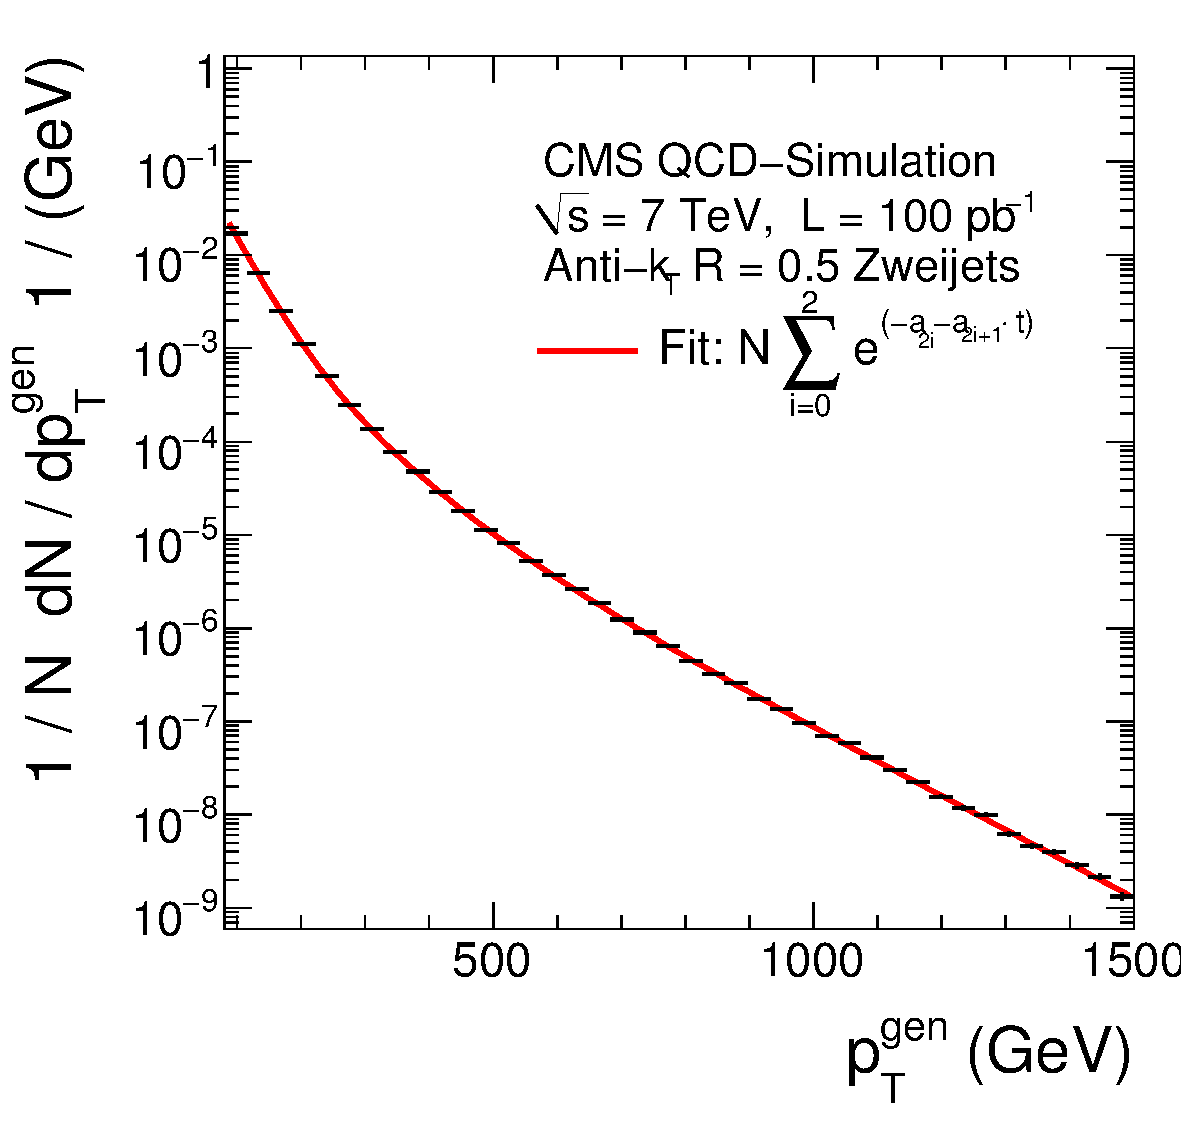
\includegraphics[width=0.45\textwidth]{figures/resFit_QCD_MCSpectrum}
%     } \subfigure[]{
%       \label{fig:resFit:qcd:dijetspectrum:subB}
%       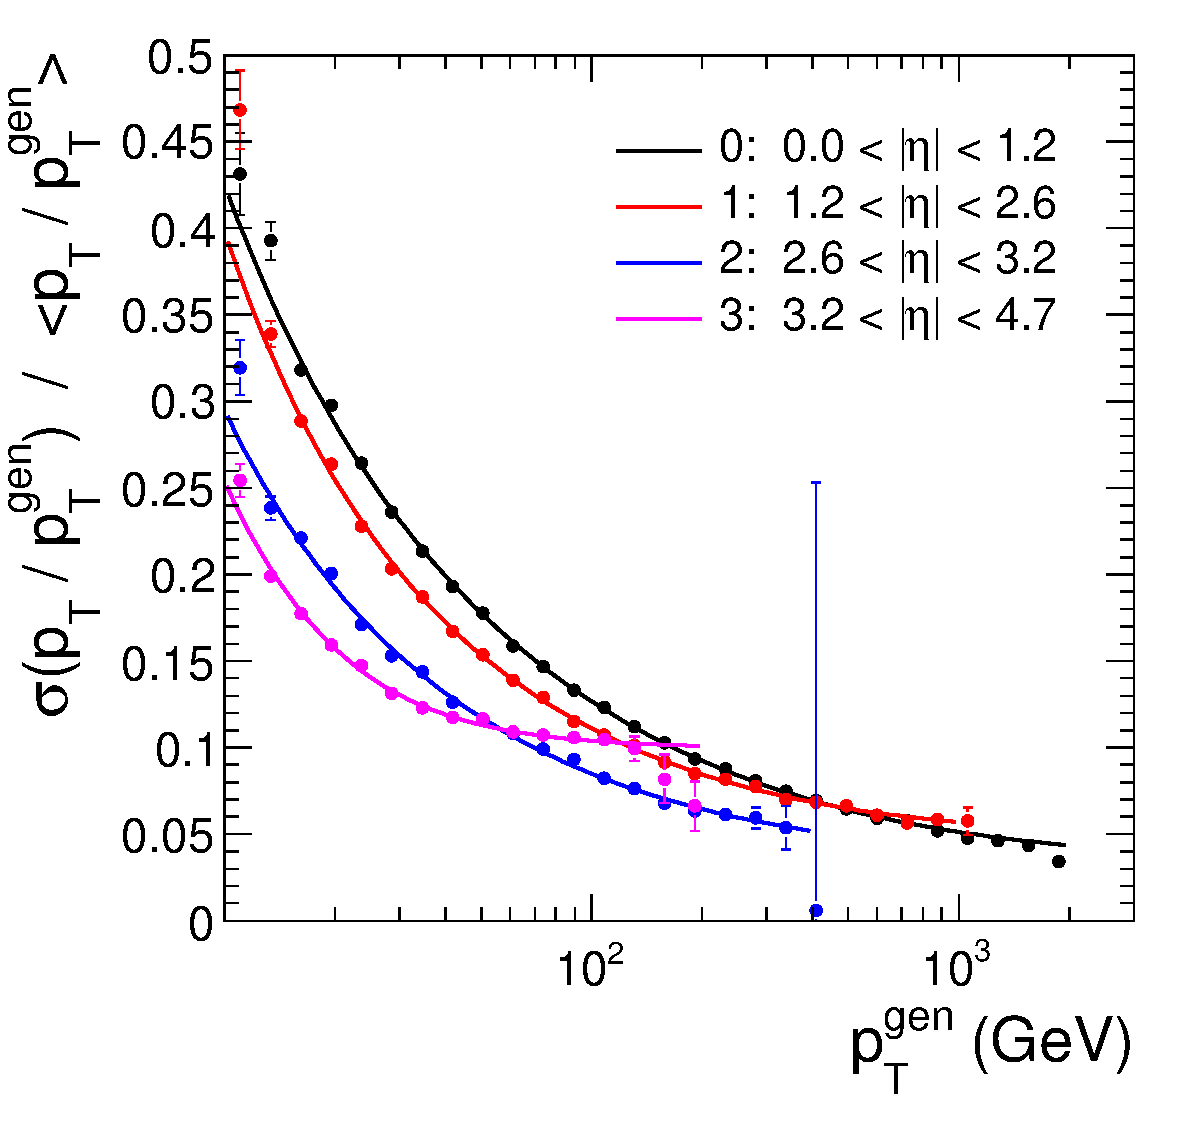
\includegraphics[width=0.45\textwidth]{figures/resFit_QCD_MCTruthResolution}
%     }
%   \end{center}
%   \caption{(a) \ptparticle distribution and (b) MC truth resolution of the leading two jets in the selected dijet sample.
%     The solid lines are fits of the indicated functions.}
%   \label{fig:resFit:qcd:dijetspectrum}
% \end{figure}

% In the following jets are considered to be ordered in corrected \ptreco.
% Dijet events are selected by requiring the third jet to have small \pt compared to the leading two jets,
% \begin{enumerate}
% \item $\ptrel < 0.1$ with $\ptrel = \frac{2\ptsub{3}}{\ptsub{1} + \ptsub{2}}$.
% \end{enumerate}
% This selection cut has been adopted from~\cite{CMSAN-2008/031}.
% The additional cut on $\Delta\phi$ performed there has been dropped as it has been found to be strongly correlated to the cut on \ptrel.
% In order to reject jets clustered from calorimeter noise a cut on the electromagnetic fration of the two leading jets is applied,
% \begin{enumerate}
% \item[2.] $0.01 < f_{\text{em},i} < 0.99$ with $i\in\{1,2\}$.
% \end{enumerate}

% So far and in the following, the resolution is defined as a function of jet \pt.
% It is influenced for example by the magnetic solenoid field which bends charged particles out of the jet cone depending on their \pt.
% Other effects such as the intrinsic calorimeter resolution are energy $E$ dependent.
% The dependence on the difference between the $E$ and \pt is minimised by considering dijet events with both leading jets in a restricted $\eta$ region,
% \begin{enumerate}
% \item[3.] $|\eta_{i}| < 1.2$ with $i\in\{1,2\}$.
% \end{enumerate}
% It is planned to apply the method to different $\eta$ regions taking into account also those events in which the two leading jets are in different $\eta$ regions.

% The events are weighted corresponding to an integrated luminosity of $100\,\text{pb}^{-1}$.

% The resulting \ptparticle spectrum is shown in Fig.~\ref{fig:resFit:qcd:dijetspectrum:subA}.
% It is fitted with an empiric function
% \begin{equation}
%   \label{eq:resFit:qcd:ptGenSpectrum}
%   f\left(\ptparticle\right) = \sum^{2}_{i=0}\,\exp\left[-\left(a_{2i} + a_{2i+1}\ptparticle\right)\right]
% \end{equation}
% to have a first applicable parameterisation of the spectrum $f(\pttrue)$.
% The fitted parameter values $a_{i}$ are listed in Table~\ref{tab:resFit:qcd:dijetspectrum} and the resulting pdf is superimposed in Fig.~\ref{fig:resFit:qcd:dijetspectrum:subA}.
% \begin{table}[ht]
%   \centering
%   \begin{tabular}{rc}
%     \hline
%     \hline
%     $a_{i}$ & Fitted value \\
%     \hline
%     $0$ & $0.56 \pm 0.04$ \\
%     $1$ & $0.0300 \pm 0.0004$ \\
%     $2$ & $3.91 \pm 0.09$ \\
%     $3$ & $0.0152 \pm 0.0004$ \\
%     $4$ & $7.15 \pm 0.05$ \\
%     $5$ & $0.00837 \pm 0.00008$ \\
%     \hline
%     \hline
%   \end{tabular}
%  \caption{Fitted parameter values of the dijet \ptparticle spectrum.}
%   \label{tab:resFit:qcd:dijetspectrum}
% \end{table}

% \begin{figure}[ht]
%   \centering
%   \includegraphics[width=0.45\textwidth]{figures/resFit_PtDependentSigma}
%   \caption{Width $\sigma$ of a Gaussian resolution in QCD dijet events. Shown is $\sigma$ from fitted parameter values (red line) in comparison to the truth from the MC simulation (blue line).}
%   \label{fig:resFit:qcd:ptDependentSigma}
% \end{figure}

% The determination of a Gaussian resolution~\eqref{eq:resFit:toyMCRes} with a \pt dependent width $\sigma$ as in~\eqref{eq:resFit:toyMCSigma} has been performed as for the ideal sample above.
% The results are not satisfying (comp. Fig.~\ref{fig:resFit:qcd:ptDependentSigma}).

% Various test have been performed and the method appears to work fine for a moderately falling \pt spectrum.
% In case of a realistic QCD spectrum (comp. Fig.~\ref{fig:resFit:qcd:dijetspectrum:subA}), however, the
% determined resolution does not describe the true resolution at large \pt anymore.
% The failure of the method is assumed to be due to the non-ideal topology of the selected dijet events, namely the presence of a third jet.
% These effects and an extension of the presented method are under study.
% Meanwhile a modified strategy to determine the resolution is investigated and presented in the following sections.


% \section{Determination of the mean Gaussian resolution in \pt bins}
% \subsection{Strategy}
% The mean Gaussian resolution with constant width $\bar{\sigma}$ is to be determined in bins of \pt.
% Afterwards it is interpolated between the bins with a continuous function.
% The bin size is chosen as a compromise between having small bins for a differential measurement and sufficient statistics in each bin.

% Dijet events are selected by the cuts described in Section~\ref{sec:resFit:qcdSelection} from the same QCD sample.
% Bins are defined by cuts on the measured jet \pt as described in Section~\ref{sec:resFit:dataDrivenExt}.
% Table~\ref{tab:resFit:qcd:ptBins} lists the chosen binning.

% \begin{table}[ht]
%   \centering
%   \begin{tabular}{rcc}
%     \hline
%     \hline
%     Bin & \ptmin (\gev) & \ptmax (\gev) \\
%     \hline
%     0 & 100 & 120 \\
%     1 & 120 & 140 \\
%     2 & 140 & 170 \\
%     3 & 170 & 200 \\
%     4 & 200 & 250 \\
%     5 & 250 & 300 \\
%     6 & 300 & 400 \\
%     7 & 400 & 600 \\
%     8 & 600 & 1000 \\
%     \hline
%     \hline
%   \end{tabular}
%   \caption{Definition of \pt bins for the fit of the mean Gaussian resolution.}
%   \label{tab:resFit:qcd:ptBins}
% \end{table}

% The modified spectrum $\tilde{f}(\pttrue)$ from~\eqref{eq:resFit:toyMC:ptCuts:extendedSpectrum} is utilised in the fit.
% The underlying spectrum $f(\pttrue)$ is described by~\eqref{eq:resFit:qcd:ptGenSpectrum} with the parameter values listed in Tab.~\ref{tab:resFit:qcd:dijetspectrum}.
% Cut-off effects are included as before using the true -- and \pt dependent -- resolution $f_{\text{MC}}(x|\pttrue)$ in $\tilde{f}(\pttrue)$.
% $f_{\text{MC}}(x|\pttrue)$ has been determined by fitting the $\ptreco/\ptparticle$ distributions in small $\ptparticle$ bins with a central Gaussian.
% The widths of the Gaussians are shown in Fig.~\ref{fig:resFit:qcd:dijetspectrum:subB}.
% They are fitted with the continous function
% \begin{equation}
%   \label{eq:resFit:qcd:sigma}
%   \frac{\sigma}{\pt} = \frac{b_{1}\sqrt{\gev}}{\sqrt{\pt}} \oplus \frac{b_{2}\gev}{\pt}.
% \end{equation}
% (In this \pt range there is no sensitivity to a third term $b_{0}$, which is why it is omitted.)
% The values $b_{i}$ of the true resolution\footnote{The fit is applied once to the presented Fig.~\ref{fig:resFit:qcd:dijetspectrum:subB} and once to an analogue plot with a logarithmic binning in \ptparticle.
% The parameters listed in Tab.~\ref{tab:resFit:qcd:resolution} are the mean values from the two fits.}
% are listed in Tab.~\ref{tab:resFit:qcd:resolution}.

% Figure~\ref{fig:resFit:qcd:specExBin} shows the \ptparticle spectrum in an example bin.
% It is well described by $\tilde{f}(\pttrue)$.


% \subsection{Results for a QCD simulation}
% \begin{figure}[ht]
%   \begin{center}
%     \subfigure[]{
%       \label{fig:resFit:qcd:specExBin}
%       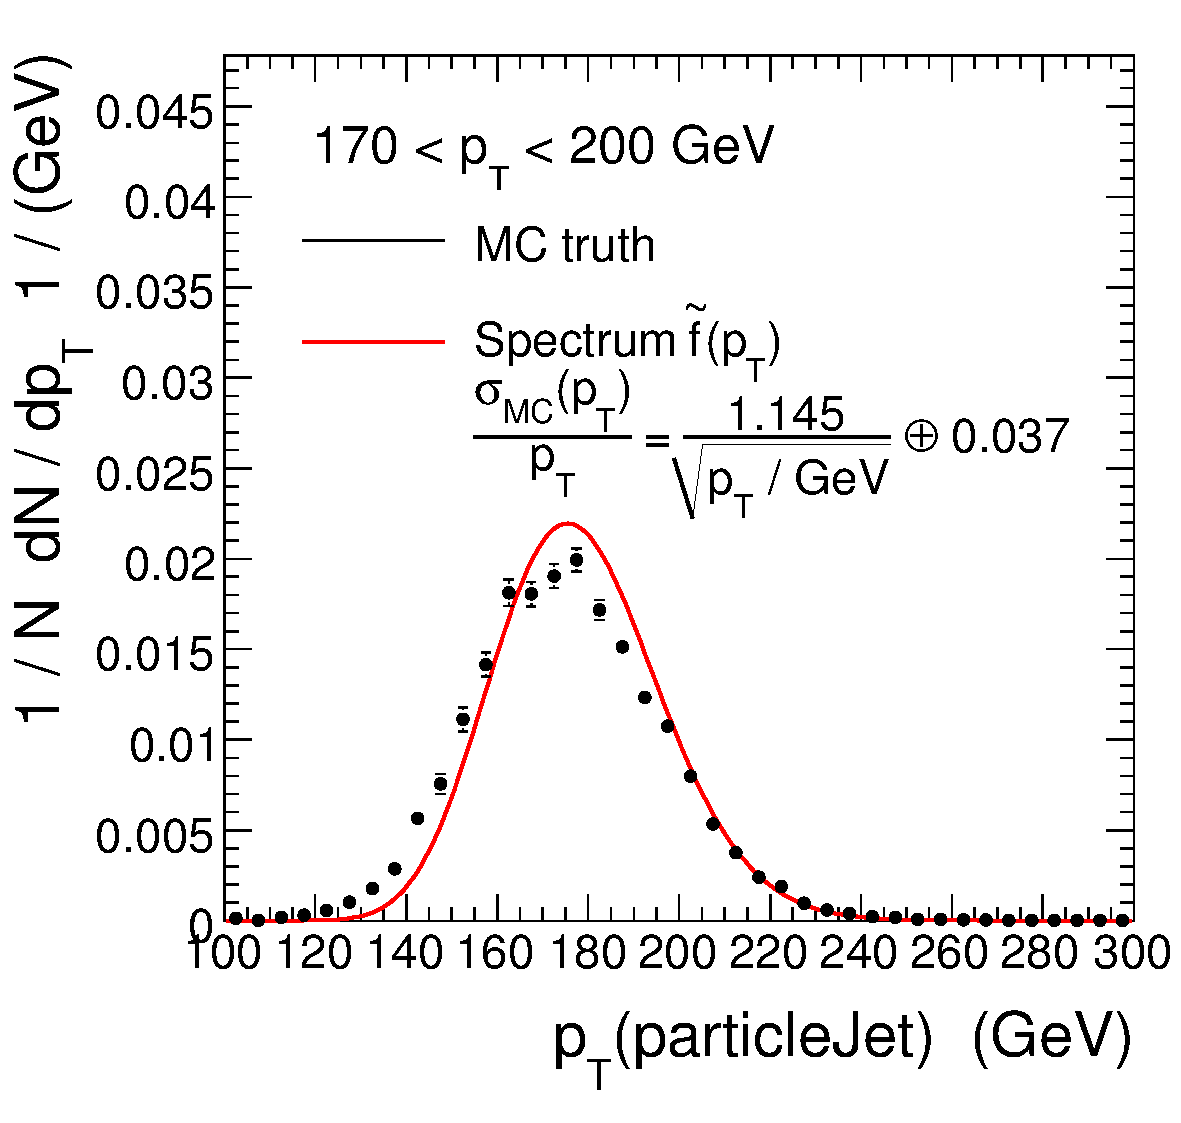
\includegraphics[width=0.45\textwidth]{figures/resFit_QCD_Gauss_Spectrum_PtBin3}
%     } \subfigure[]{
%       \label{fig:resFit:qcd:extrapolationExBin}
%       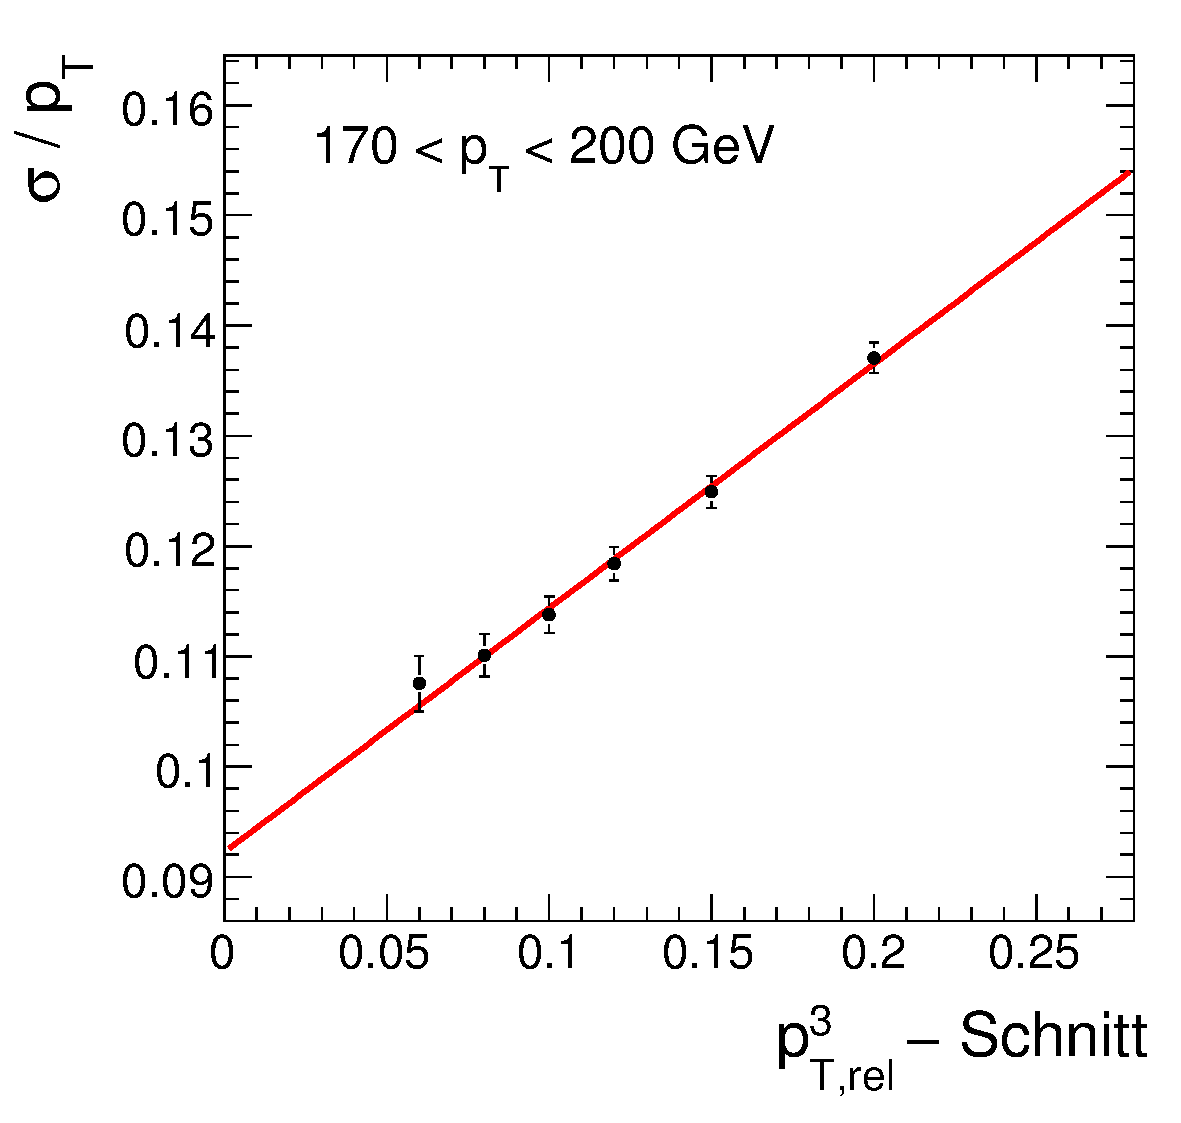
\includegraphics[width=0.45\textwidth]{figures/resFit_QCD_Gauss_ExtrapolatedSigma_PtBin3}
%     }
%   \end{center}
%   \caption{(a) \ptparticle distribution and of the leading two jets in an example \pt bin.
%     The solid line is the spectrum $\tilde{f}(\pttrue)$.
%     (b) Fitted Gaussian mean widths $\bar{\sigma}/\pt$ for different cuts on \ptrel in the same example \pt bin.
%     The solid line is a linear fit to extrapolate $\bar{\sigma}/\pt$ for ideal dijet events.}
% \end{figure}

% The fit has been performed for the listed \pt bins.
% The result is affected by the presence of a third jet.
% For example, the mean resolution for jets with \mbox{$170 < \ptreco < 200\gev$} has been determined to \mbox{$\bar{\sigma}/\bar{\pt} = 0.136 \pm 0.002$} whereas the MC truth value is \mbox{$0.0933$}.
% This difference is dependent on the maximum \ptrel as demonstrated in Fig.~\ref{fig:resFit:qcd:extrapolationExBin}, which shows the fitted mean resolution for different values of \ptrel.
% There is a linear trend visible.
% In order to extrapolate to the results to the case of an ideal dijet event, the $\bar{\sigma}\/\pt$ are fitted with a linear function and the y axis intercept is considered as the correct jet energy resolution.

% The extrapolated Gaussian mean widths $\bar{\sigma}/\pt$ found in this way are shown for different \pt bins in Fig.~\ref{fig:resFit:qcd:extrapolation}.
% Here, the \pt values are the mean values of the assumed spectra $\tilde{f}(\pttrue)$ in each bin.
% The shown statistical uncertainties are combined from two sources.
% \begin{enumerate}
% \item The first contribution is the statistical uncertainty on the parameter of y axis intercept in the linear extrapolation (comp. Fig.~\ref{fig:resFit:qcd:extrapolationExBin}).
% \item The second contribution arises from the uncertainty due to the statistics in the used MC sample.
%   As the event weights are large for small \pt, statistical fluctations might become significant.
%   In order to roughly evaluate this uncertainty, the same fits have been performed again without event weights (for the used sample this corresponds to a flattened QCD spectrum).
%   The statistical uncertainties obtained in this case on the y axis intercept are added in quadrature to the ones in 1.
%   This procedure has to be improved to obtain a statistically correct description of the uncertainty.
% \end{enumerate}

% The dashed line in Fig.~\ref{fig:resFit:qcd:extrapolation} represents the MC truth resolution.
% The fitted values are in reasonable agreement with the MC truth.
% They are then fitted with the continous function \eqref{eq:resFit:qcd:sigma} (solid line).
% The parmeters of this fit are listed in Tab.~\ref{tab:resFit:qcd:resolution}.

% \begin{table}[ht]
%   \centering
%   \begin{tabular}[ht]{lcc}
%     \hline \hline
%     $b_{i}$ & $1$ & $2$ \\
%     \hline
%     MC truth    & $1.145 \pm 0.001$ & $0.0370 \pm 0.0006$ \\
%     Fit result  & $1.18  \pm 0.04$  & $0.032  \pm 0.007$ \\
%     \hline \hline
%   \end{tabular}
%   \caption{Parameter values of the width $\sigma(\pt)$ of the Gaussian resolution~\eqref{eq:resFit:qcd:sigma}.
%     Listed are the MC truth values and the fitted values.
%     For the fit, the mean $\bar{\sigma}/\pt$ has been fitted in different \pt bins and the result fitted again with the continous function~\eqref{eq:resFit:qcd:sigma} (comp. Fig.~\ref{fig:resFit:qcd:extrapolation}).
%     The uncertainties assigned to the fitted values are the statistical uncertainties.}
%   \label{tab:resFit:qcd:resolution}
% \end{table}

% \begin{figure}[ht]
%   \begin{center}
%     \subfigure[]{
%       \label{fig:resFit:qcd:extrapolation}
%       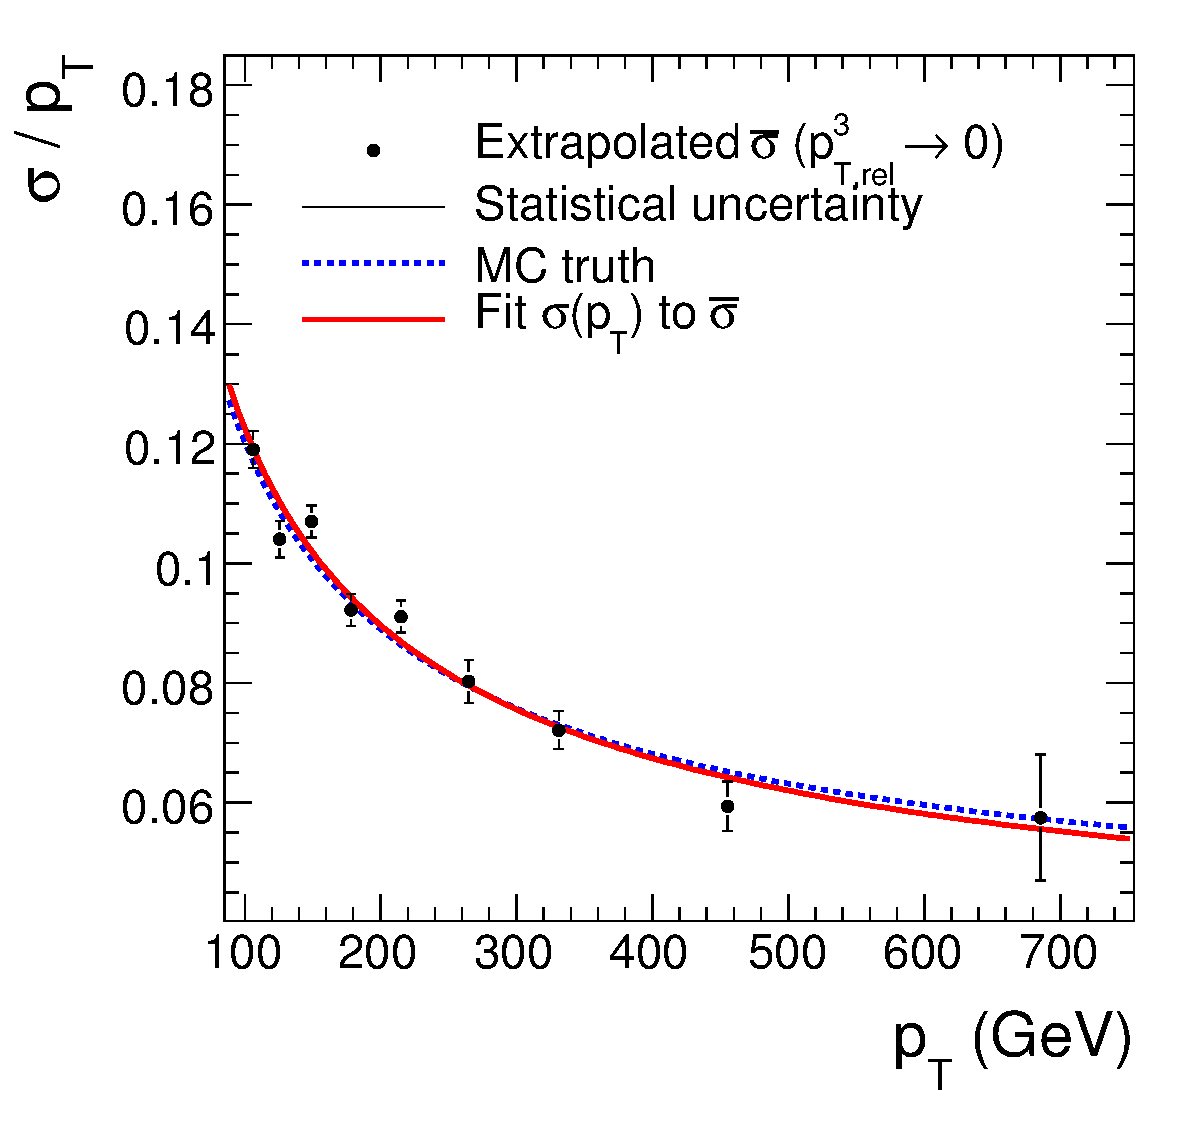
\includegraphics[width=0.45\textwidth]{figures/resFit_QCD_Gauss_ExtrapolatedResolution}
%     } \subfigure[]{
%       \label{fig:resFit:qcd:systUncert}
%       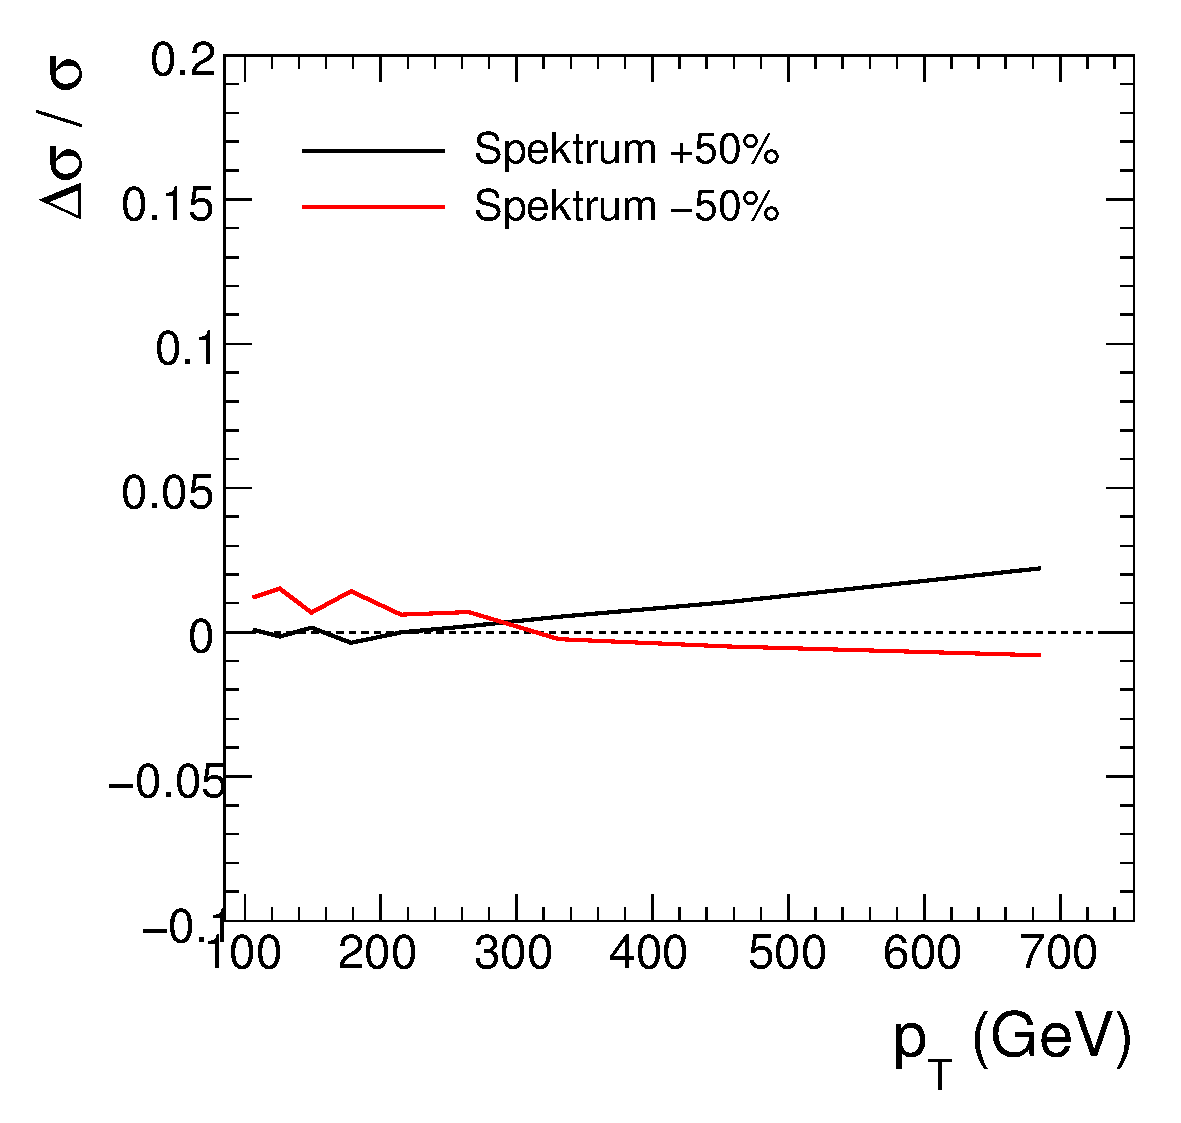
\includegraphics[width=0.45\textwidth]{figures/resFit_QCD_Gauss_SystematicUncertainties}
%     }
%   \end{center}
%   \caption{(a) Gaussian mean widths $\bar{\sigma}/\pt$ from extrapolation \mbox{$\ptrel\rightarrow0$} in different \pt bins.
%   The \pt values are the mean values of the assumed spectra $\tilde{f}(\pttrue)$ in each bin.
%   The error bars indicate the combined statistical uncertainties from the extrapolation and the MC statistics.
%   The solid line is a fit to the $\bar{\sigma}/\pt$, the dashed line shows the MC truth resolution for comparison.
%   (b) Estimation of systematic uncertainties.
%   The lines represent relative differences of the resolution for different variations of the spectrum to the correct spectrum.}
% \end{figure}
% \clearpage


% \section{Determination of a non-Gaussian resolution}

% \subsection{\mht spectrum from Gaussian resolution}
% In order to evaluate the influence of non-Gaussian tails in the resolution to the \mht spectrum, a simple generator level based jet smearing has been performed.
% The same dijet selection as presented in Sec.~\ref{sec:resFit:qcdSelection} has been applied.
% For this demonstration, the \ptparticle of the leading two jets has been weighted with a random number from a Gaussian resolution pdf, where $\sigma$ has been parameterised using the MC truth values listed in Tab.~\ref{tab:resFit:qcd:resolution}.

% \begin{figure}[ht]
%   \begin{center}
%     \subfigure[]{
%       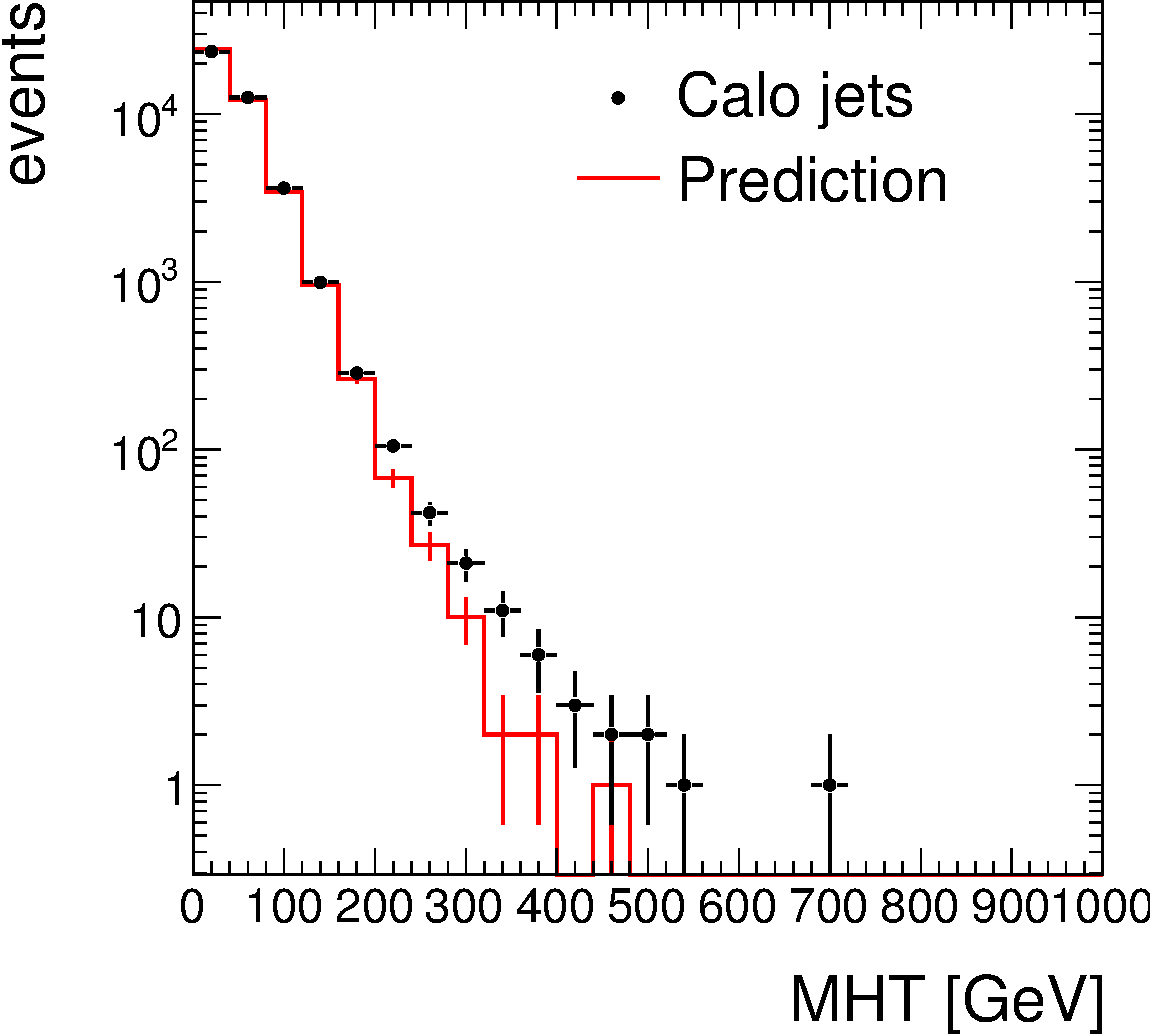
\includegraphics[width=0.45\textwidth]{figures/MHTSpectrumGauss}
%     } \subfigure[]{
%       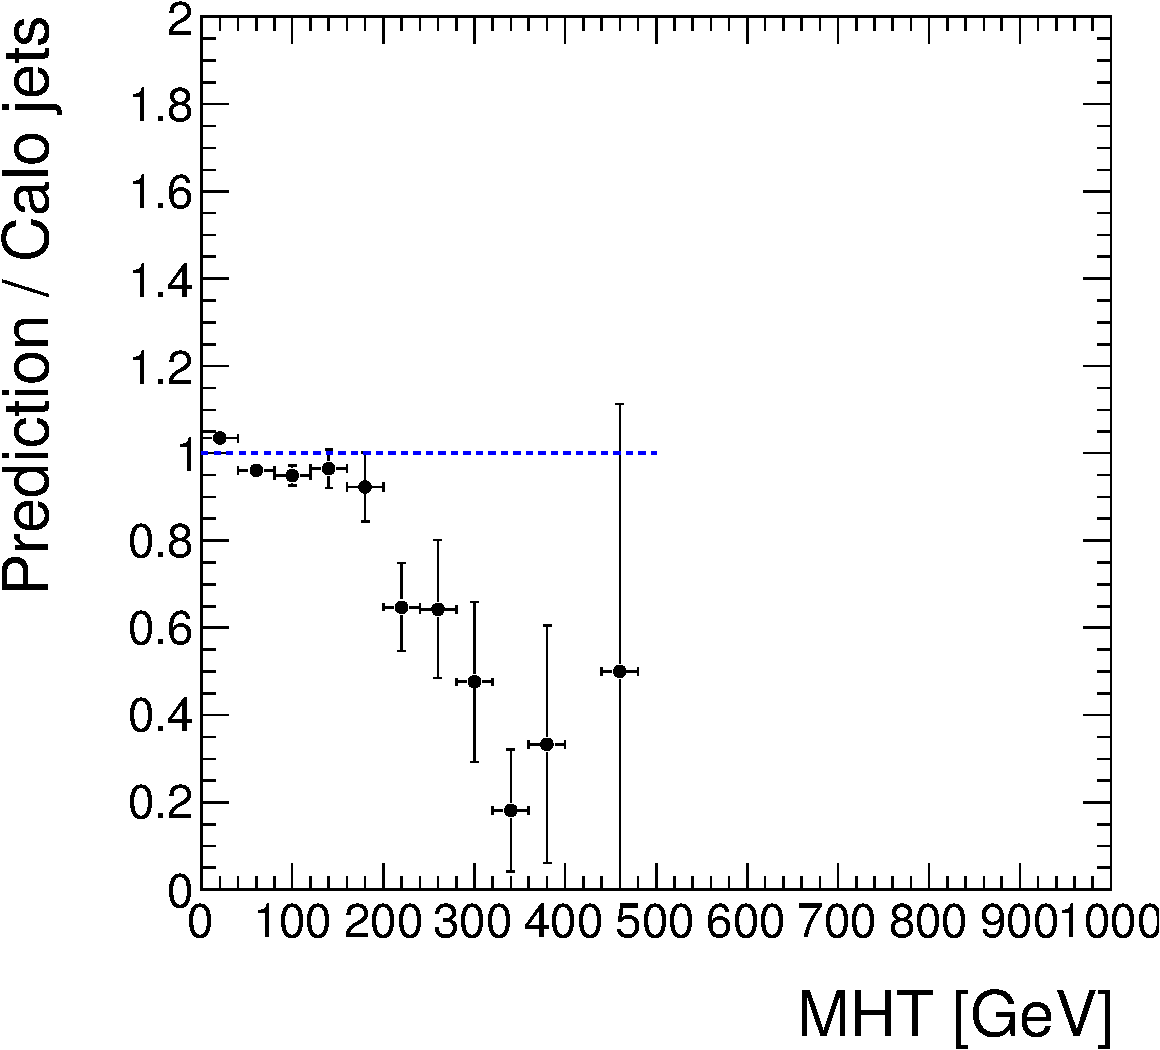
\includegraphics[width=0.45\textwidth]{figures/MHTRatioGauss}
%     }
%   \end{center}
%   \caption{(a) \mht from the two leading jets in a QCD dijet sample (marker) and prediction from smearing of the corresponding generator level jets with the true Gaussian resolution (line).
%     (b) Ratio of prediction and truth.}
% \label{fig:resFit:qcd:mhtGauss}
% \end{figure}

% In Fig.~\ref{fig:resFit:qcd:mhtGauss} the \mht spectrum resulting from
% the weighted \ptparticle of the two jets is compared to the \mht spectrum from the corresponding \ptreco.
% The actual \mht is underestimated by about $5\%$ up to 200\gev.
% Above, which are $\approx2\%$ of all the events, the \mht is underestimated by $\approx50\%$.
% This difference is explained by the presence of non-Gaussian tails in the resolution which were not considered.

% In conclusion, it is necessary to include the description of non-Gaussian tails of the resolution into the fit in order to accurately predict the \mht spectrum using a smearing method.


% \subsection{Parameterisation of the resolution by a Crystal Ball function}
% \textit{to be added}



% ----- Bibliography ------------------------------------

\begin{thebibliography}{9}
\bibitem{CMSAN-2008/031} \texttt{CMS AN-2008/031}, \textit{Determination of the Relative Jet Energy Scale at CMS from Dijet Balance}, (2008)
\end{thebibliography}



\end{document}
